\documentclass{beamer}
\usepackage[latin1]{inputenc}
\usepackage{color}
\usepackage{multirow}
%\usepackage[pdftex]{graphicx}
%\usepackage{sidecap}
%\usepackage{siunitx}
%\usepackage{epstopdf}
\setbeamertemplate{footline}[frame number]
\usetheme{default}
\title{The Measurement of \\ the W$\gamma$ Cross Section at 8 TeV \\ (PhD thesis defense) }
\author{Ekaterina Avdeeva}
\institute{University of Nebraska - Lincoln}
\date{June, 2017}



\begin{document}

\begin{frame}
\titlepage % Title
\end{frame}

\begin{frame}\frametitle{Talk Outline}
  \begin{itemize}
     \item {\scriptsize\bfseries{Introduction to theory}}
       \begin{itemize}
          \tiny
          \item Standard Model
          \item Proton-proton collisions
          \item $W\gamma\rightarrow l\nu\gamma$ process
       \end{itemize}
     \item {\scriptsize\bfseries{Experimental setup}}
       \begin{itemize}
          \tiny
          \item Large Hadron Collider (LHC)
          \item Compact Muon Solenoid (CMS)
          \item Particle reconstruction in CMS
       \end{itemize}
     \item {\scriptsize\bfseries{$W\gamma$ cross section measurement}}
       \begin{itemize}
          \tiny
          \item Data
          \item Measurement steps
          \item {\bfseries{Main challenge:}} jets$\rightarrow\gamma$ background estimation
          \item Systematic uncertainties
          \item Results
       \end{itemize}
%     \item {\scriptsize\bfseries{Acknowledgements}}
     \item {\scriptsize\bfseries{Conclusions}}
  \end{itemize}

  \tiny
  More details about each subject are available in the dissertation:\\
  https://github.com/eavdeeva/ThesisTextWg/blob/master/nuthesis/examples/nuthesis.pdf
\end{frame}%{Outline}

 % Outline, SM
\begin{frame}\frametitle{Theory. Atom Structure}
\begin{figure}[htb]
  \begin{center}
    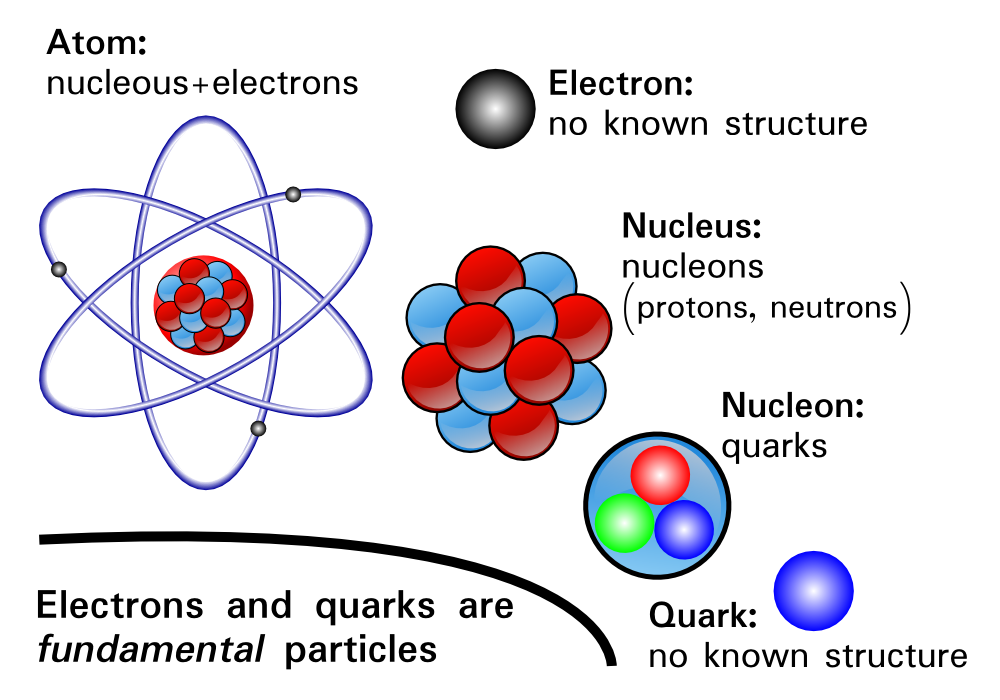
\includegraphics[width=0.98\textwidth]{../figs/ForPresentation/Theory_StandardModel01.png}
  \end{center}
\end{figure}
\tiny
http://www.nuclear-power.net/nuclear-power/reactor-physics/atomic-nuclear-physics/
\end{frame}%{Atom Structure}

\begin{frame}\frametitle{Theory. The Standard Model}
\begin{figure}[htb]
  \begin{center}
    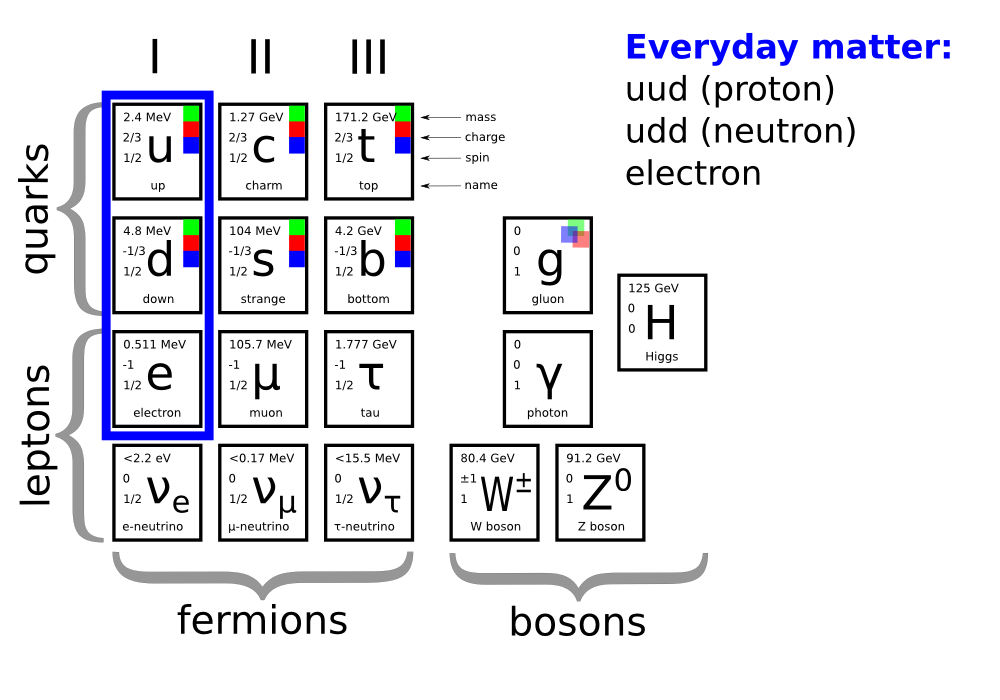
\includegraphics[width=0.98\textwidth]{../figs/ForPresentation/Theory_StandardModel02.png}
  \end{center}
\end{figure}
\tiny
http://www.nuclear-power.net/nuclear-power/reactor-physics/atomic-nuclear-physics/
\end{frame}%{The Standard Model}

\begin{frame}\frametitle{Theory. Proton-Proton Collisions}
\begin{figure}[htb]
  \begin{center}
    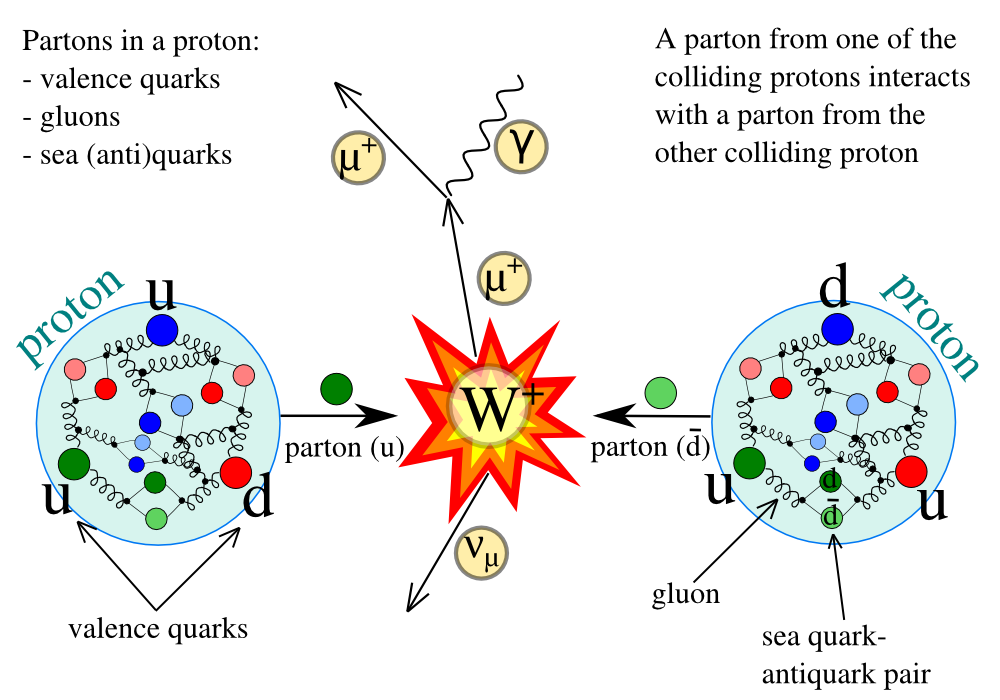
\includegraphics[width=0.60\textwidth]{../figs/ForPresentation/Theory_ppCollision.png}
  \end{center}
\end{figure}
\scriptsize
\begin{itemize}
  \item Quarks u,u,d within a proton interact and produce gluons and quark-antiquark pairs;
  \item In a $pp$ collision, any ``parton'' from one proton can interact with any parton from another proton.
\end{itemize}
\tiny
http://cms.web.cern.ch/news/weak-mixing-light-and-heavy
\end{frame}%{Proton-Proton Collisions}

\begin{frame}\frametitle{Theory. $W\gamma\rightarrow l\nu\gamma$}
   \begin{figure}[htb]
      \begin{center}
        \scriptsize
          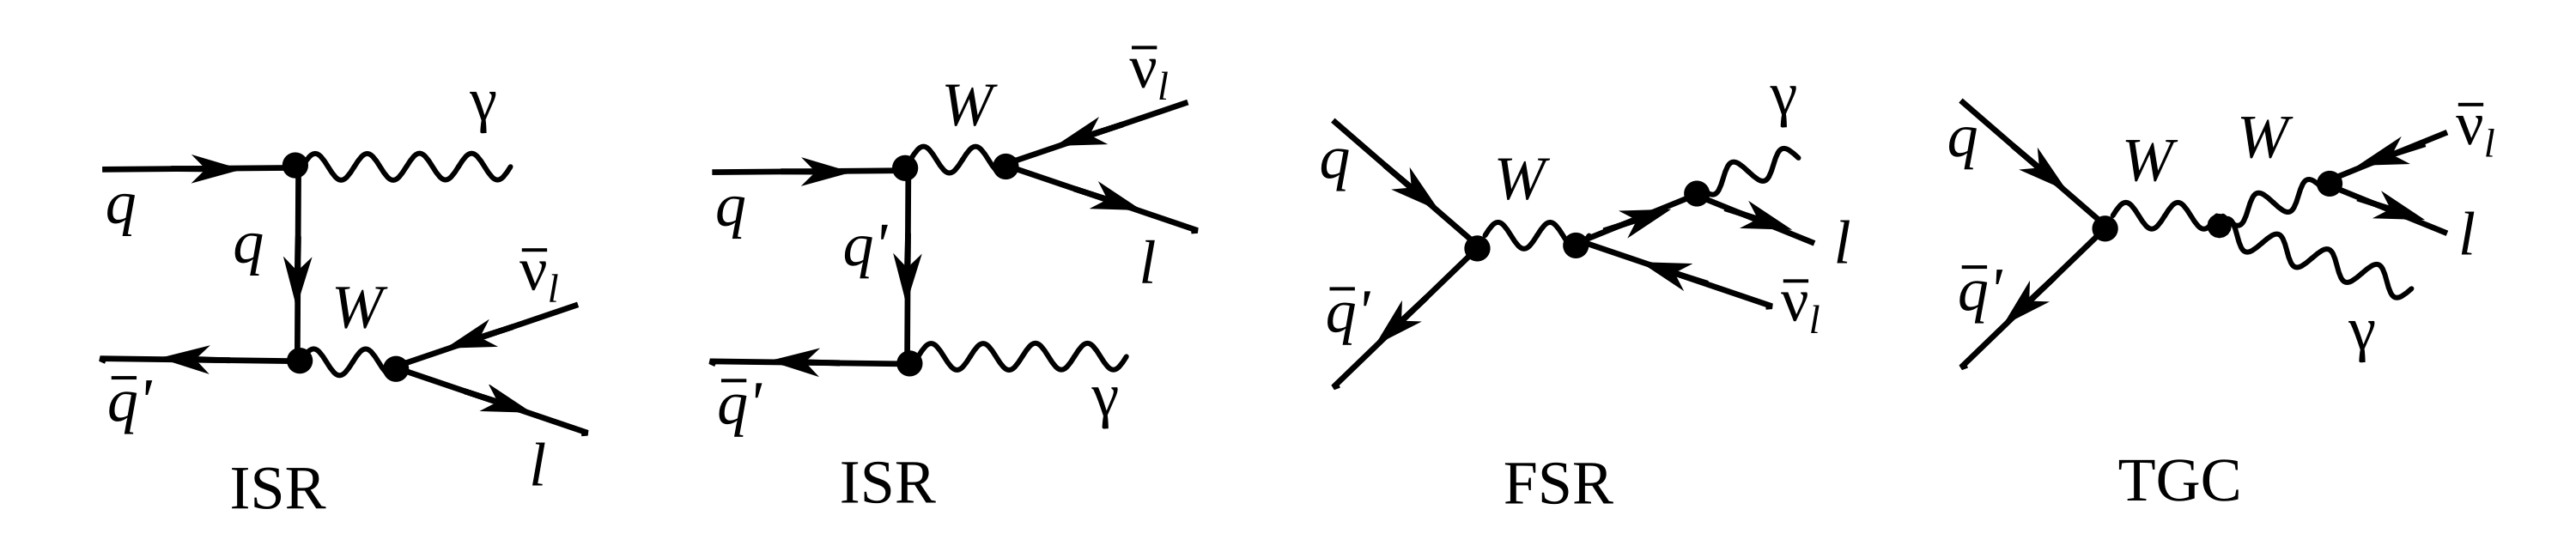
\includegraphics[width=0.95\textwidth]{../figs/ForPresentation/feynmWg_LO_01.png}
%          \caption{\scriptsize{The Feynman diagrams. ISR(x2), FSR, and TGC.}}
       \end{center}
    \end{figure}
\scriptsize
$q_1\bar{q_2}\rightarrow W$ or $q_1\bar{q_2}\rightarrow W\gamma$\\
Usually $q_1\bar{q_2}=u\bar{d}$ or  $q_1\bar{q_2}=d\bar{u}$\\

\begin{table}[h]
  \scriptsize
  \begin{center}
   \begin{tabular}{|l|l|}
    \hline
         &  \\ 
     {\bfseries{Three mechanisms:}}  & {\bfseries{Measurement goals:}}  \\
         &  \\ 
     ISR: initial state radiation;   & Test the Standard Model;  \\ 
     FSR: final state radiation;    &  Provide a precise cross section measurement; \\ 
     TGC: triple gauge coupling.    &  Search for anomalous TGC (aTGC).\\ 
    &  \\  \hline
  \end{tabular}
  \end{center}
\end{table}

\end{frame}%{Theory. $W\gamma\rightarrow l\nu\gamma$}

\begin{frame}\frametitle{Theory. $W\gamma\rightarrow l\nu\gamma$}
   \begin{figure}[htb]
      \begin{center}
        \scriptsize
          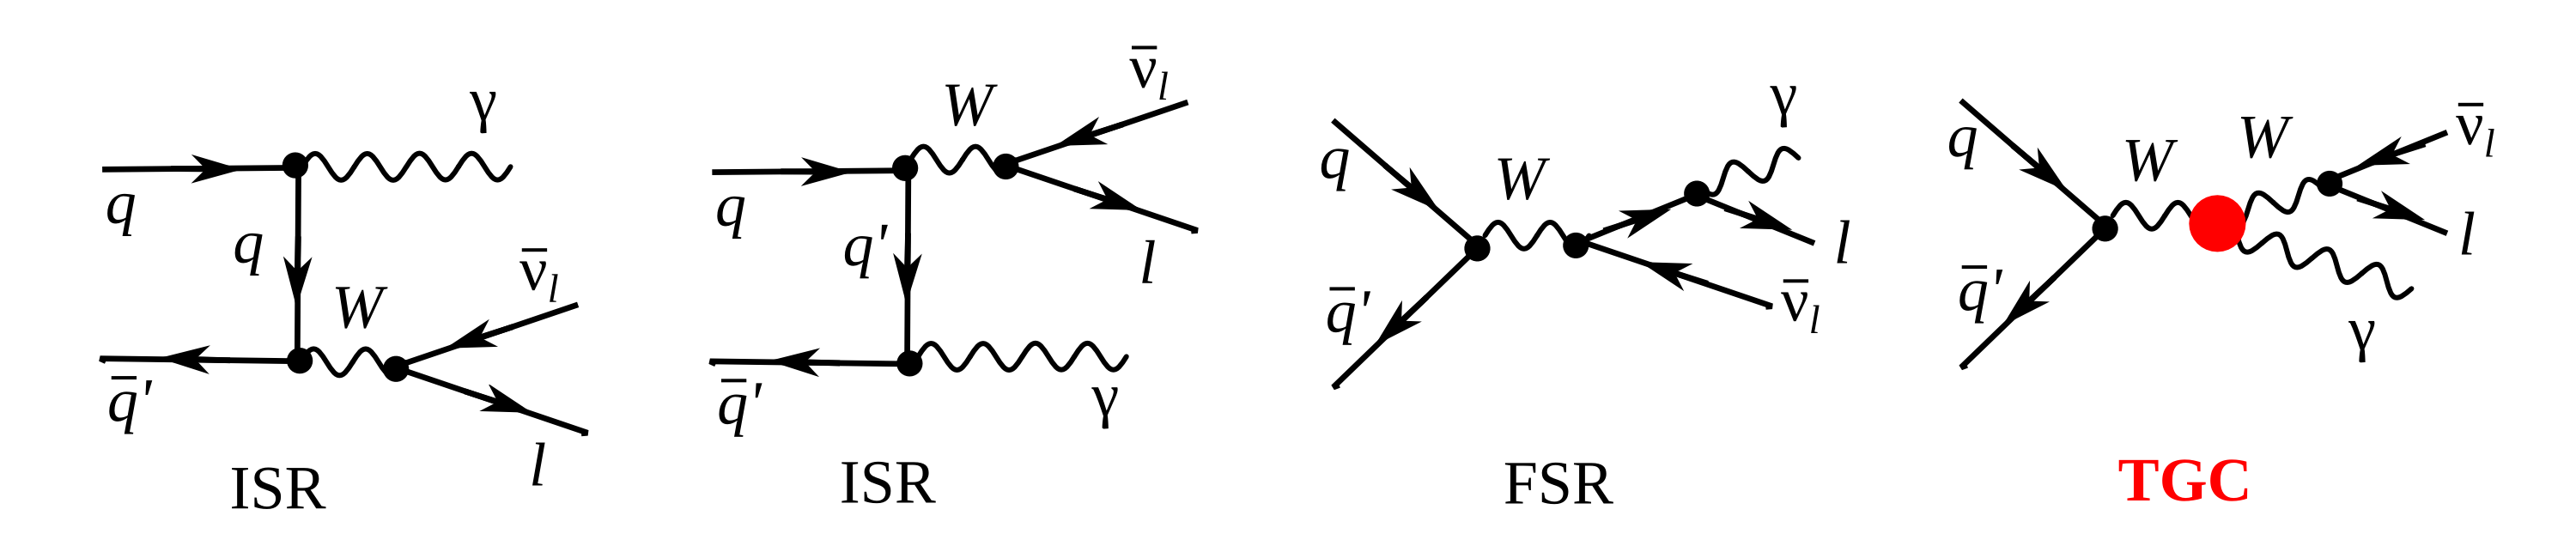
\includegraphics[width=0.95\textwidth]{../figs/ForPresentation/feynmWg_LO_02.png}
%          \caption{\scriptsize{The Feynman diagrams. ISR(x2), FSR, and TGC.}}
       \end{center}
    \end{figure}
\scriptsize
$q\bar{q'}\rightarrow W$ or $q\bar{q'}\rightarrow W\gamma$\\
-  \\
Usually $q\bar{q'}=u\bar{d}$ or  $q\bar{q'}=d\bar{u}$\\

\begin{table}[h]
  \scriptsize
  \begin{center}
   \begin{tabular}{|l|l|}
    \hline
         &  \\ 
     {\bfseries{Three mechanisms:}}  & {\bfseries{Measurement goals:}}  \\
         &  \\ 
     ISR: initial state radiation;   & Test the Standard Model;  \\ 
     FSR: final state radiation;    &  Provide a precise cross section measurement; \\ 
     {\color{red}{TGC: triple gauge coupling.}}    &  {\color{red}{Search for anomalous TGC (aTGC).}}\\ 
    &  \\  \hline
  \end{tabular}
  \end{center}
\end{table}

\end{frame}%{Theory. $W\gamma\rightarrow l\nu\gamma$}

 % EWK, TGC/QGC, WGamma
\begin{frame}\frametitle{Large Hadron Collider (LHC)}
  \begin{figure}[htb]
    \begin{center}
      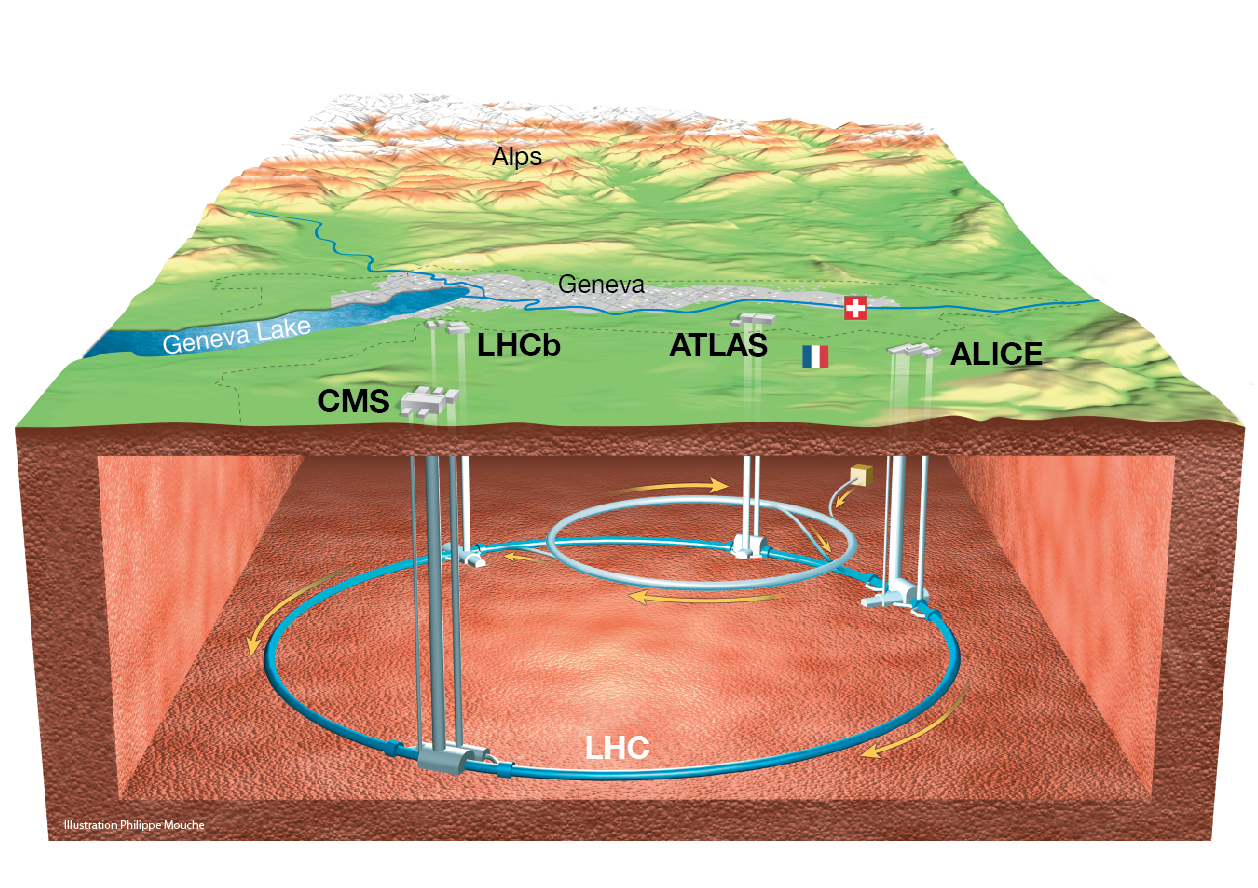
\includegraphics[width=0.80\textwidth]{../figs/ForPresentation/LHC.png}
    \end{center}
  \end{figure}
\tiny
http://lhcathome.web.cern.ch/about
\end{frame}%{Large Hadron Collider}

\begin{frame}\frametitle{Compact Muon Solenoid (CMS)}
\begin{figure}[htb]
  \begin{center}
    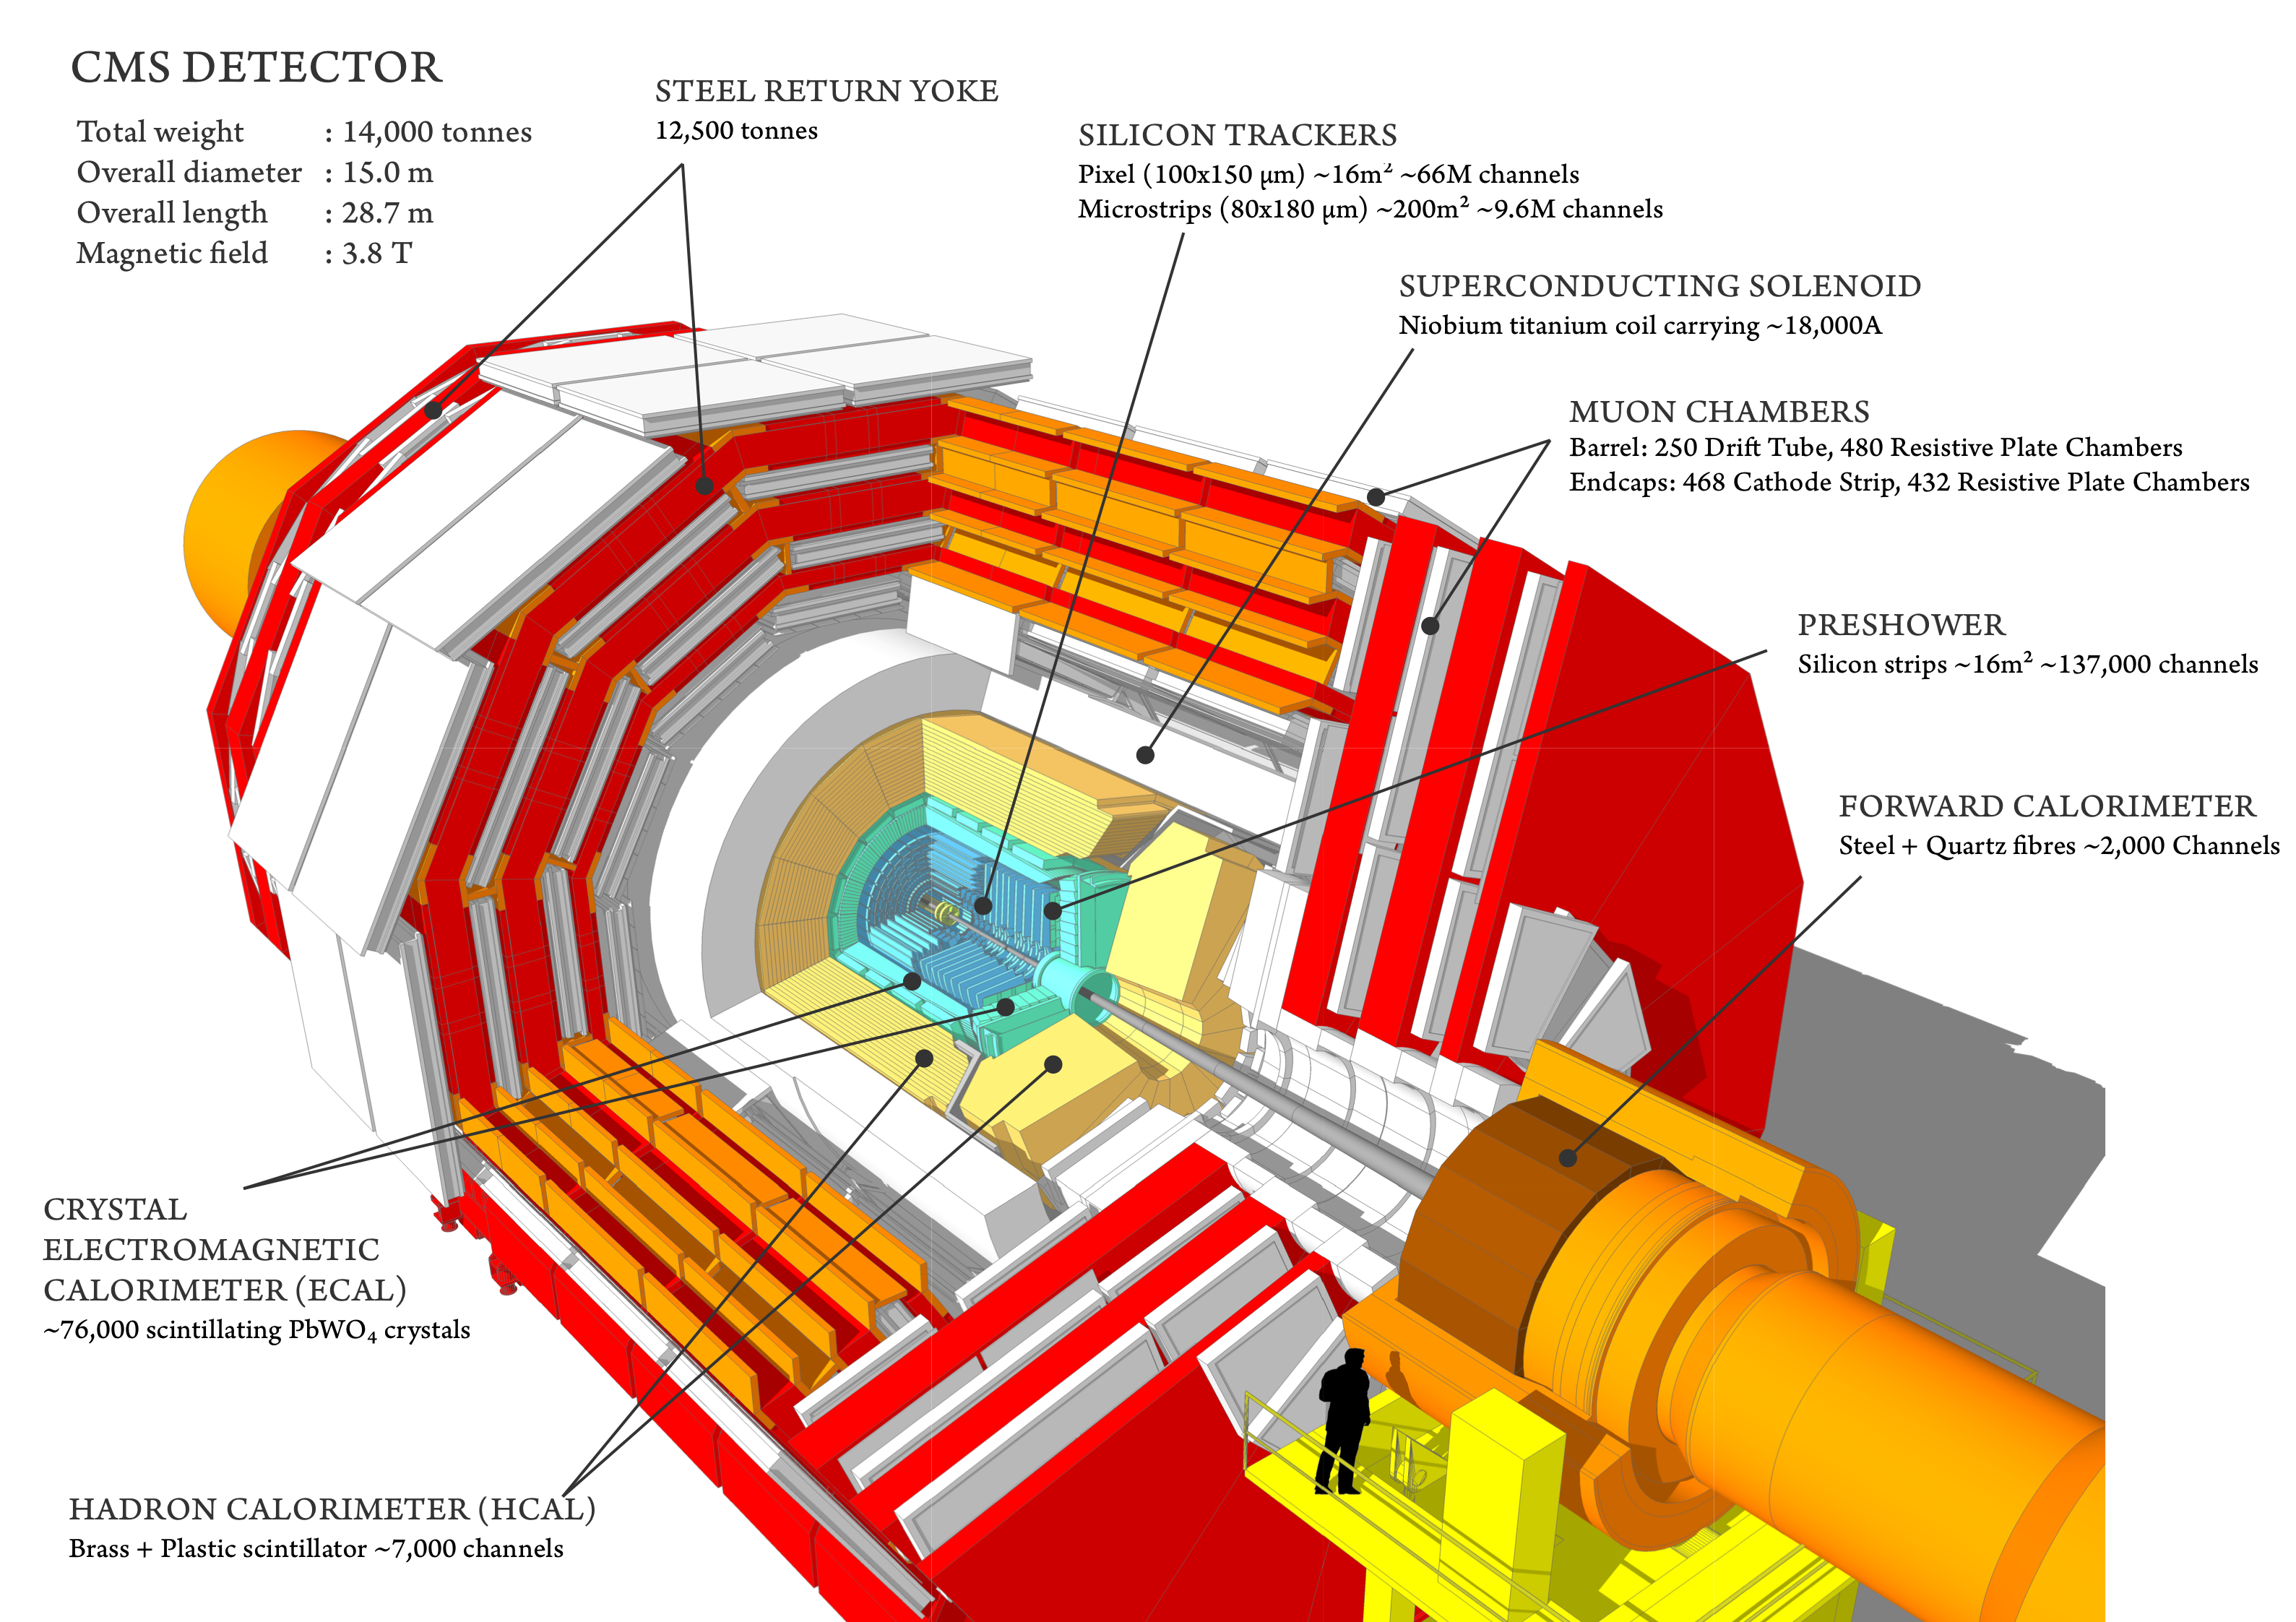
\includegraphics[width=0.90\textwidth]{../figs/ForPresentation/CMS.png}
  \end{center}
\end{figure}
\tiny
http://cms.web.cern.ch/news/cms-detector-design
\end{frame}%{Compact Muon Solenoid (CMS). Components}


\begin{frame}\frametitle{Compact Muon Solenoid (CMS). Particle Reconstruction}
\scriptsize
Process to study: $W\gamma\rightarrow\mu\nu\gamma$, $W\gamma\rightarrow e\nu\gamma$.\\
Final state particles: muons, electrons, photons, neutrinos.\\
\begin{figure}[htb]
  \begin{center}
    {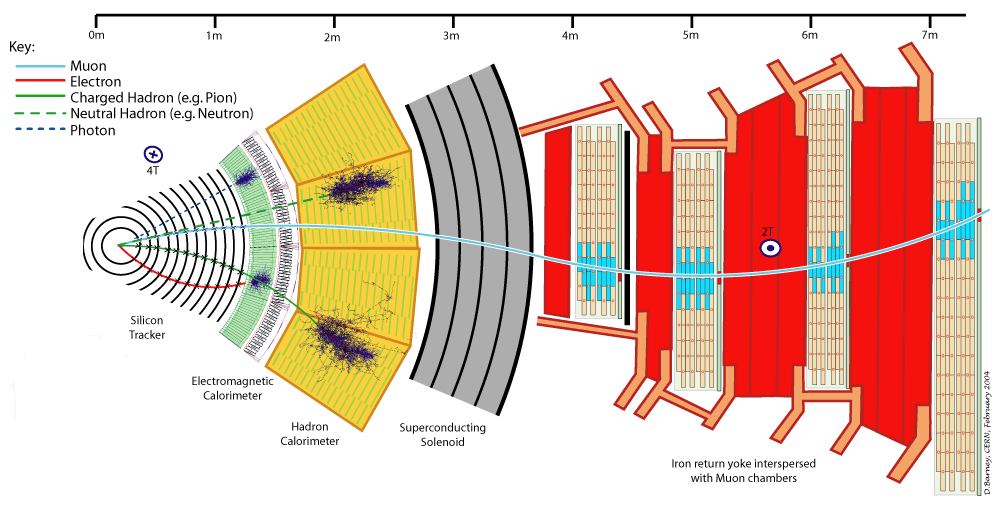
\includegraphics[width=0.80\textwidth]{../figs/Exp/CMS_Slice.png}}
  \end{center}
\end{figure}

\scriptsize
Neutrino is not detected. The measure of $P_T^{\nu}$ is\\ 
missing transverse energy: $  E_T^{miss} = - | \sum \mathbf{P_T} |$,\\
Sum over all visible particles in the event. 

\end{frame}%{Compact Muon Solenoid (CMS). Particle Reconstruction}

\begin{frame}\frametitle{Compact Muon Solenoid (CMS). Neutrinos}
\scriptsize
Process to study: $W\gamma\rightarrow\mu\nu\gamma$, $W\gamma\rightarrow e\nu\gamma$.\\
Final state particles: muons, electrons, photons, {\color{blue}\bfseries{neutrinos}}.\\
\begin{figure}[htb]
  \begin{center}
    {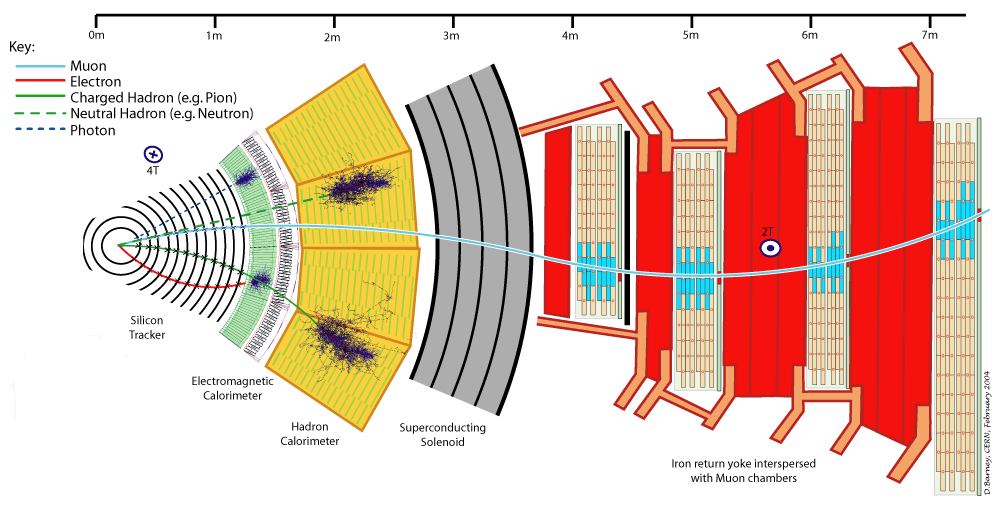
\includegraphics[width=0.70\textwidth]{../figs/Exp/CMS_Slice.png}}
  \end{center}
\end{figure}

\scriptsize
{\color{blue}\bfseries{Neutrino is not detected}}. The measure of $P_T^{\nu}$ is\\ 
{\bfseries{missing transverse energy}}: $  E_T^{miss} = - | \sum \mathbf{P_T} |$,\\
Sum over all visible particles in the event. 

\end{frame}%{Compact Muon Solenoid (CMS). Particle Reconstruction}

\begin{frame}\frametitle{Kinematic Variables and Important Notations}

\begin{figure}[htb]
  \begin{center}
    {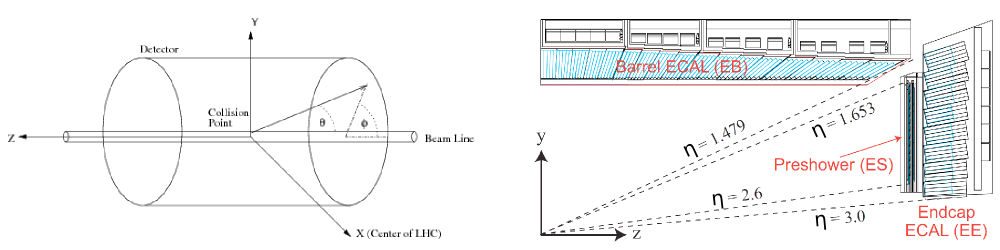
\includegraphics[width=0.90\textwidth]{../figs/ForPresentation/CMS_coordSyst_and_ECal.png}}
  \end{center}
\end{figure}

\tiny
\begin{itemize}
  \item Transverse momentum ($P_T$) with respect to the beamline
  \item Pseudorapidity ($\eta=-ln \left[ tan{(\theta/2)} \right]$)
  \item Cone separation ($\Delta R(a,b) = \sqrt( (\phi_a-\phi_b)^2 + (\eta_a-\eta_b)^2 )$)
  \item EB (barrel) and EE (endcap)
  \item Invariant mass of a particle system ($M_{ab} = m_a^2+m_b^2+2(E_aE_b-{\bfseries{p_a\cdot p_b}})$)
  \item Transverse mass of a $W$ boson ($M_T^W=\sqrt{2  P_T^{l}  E_T^{miss}  (1-\cos{(\phi^{l}-\phi^{miss})})}$)
\end{itemize}

\end{frame}%{Kinematic Variables and Important Notations}


 % LHC, pp collision, CMS, reconstruction, MET
\begin{frame}\frametitle{Measurement Goal}
  \scriptsize

  To measure the total and the differential ($\frac{d\sigma}{dP_T^{\gamma}}$) cross sections of $W\gamma\rightarrow l\nu\gamma$ at $\sqrt{s}=$8~TeV.\\
  - - - - - - - - - - - - - - - \\
  Phase space definition:
  \begin{itemize}
    \item $P_T^{\gamma}>$ 15 GeV;
    \item $\Delta{R}(\gamma,lep) > $0.7;
    \item several more requirements related to geometric and kinematic limitations
% \item $|\eta^{\gamma}|<2.5$, $|\eta^{lep}|<2.5$
%  \item $p_T^{lep}>$ 20 GeV
%  \item $Iso^{\gamma}<$ 5 GeV
%  \item for Z$\gamma$ Check: M(lep,lep)$>$50 GeV
%    \item $P_T^{\gamma}$ ranges for $\frac{d\sigma}{dP_T^{\gamma}}$: 15-20-25-30-35-45-55-65-75-85-95-120-500 GeV
  \end{itemize}
\end{frame}%{Measurement Goal}

\begin{frame}\frametitle{Measurement Strategy}
\begin{table}[h]
  \scriptsize
  \begin{center}
  \begin{tabular}{|l|c|c|}
    \hline
          & \multicolumn{2}{|c|}{Algebraic representation for} \\ 
     Step & \multicolumn{2}{|c|}{the measurement of} \\ 
          & $d\sigma/dP_{T}^{\gamma}$ & $\sigma$ \\ \hline
    {\bfseries\footnotesize{select events}} & {\bfseries{$N_{sel}^j$}} &    {\bfseries{$N_{sel}$}}       \\ \hline
    {\bfseries\footnotesize{subtract background}} & {\bfseries{$N_{sign}^j = N_{sel}^j - N_{bkg}^j$}} &    {\bfseries{$N_{sign}=N_{sel}-N_{bkg}$}}       \\ \hline
    unfold   & $N_{A\times\epsilon}^i = U_{ij} \cdot N_{sign}^j$ &    $-$       \\ \hline
    correct for efficiency & $N_{true}^i = \frac{N_{A\times\epsilon}^i}{(A \times\epsilon)^i}$ &  $N_{true}=\frac{N_{sign}}{A\times\epsilon}$       \\ \hline
    compute cross section & $ \left( \frac{d\sigma}{dP_{T}^\gamma} \right) ^i = \frac{N_{true}^i}{L \cdot (\Delta P_T^\gamma)^i}$  &  $\sigma = N_{true}/L$       \\ \hline
    \multicolumn{3}{|l|}{\bfseries\footnotesize{estimate systematic uncertainties}}          \\ \hline
  \end{tabular}
  \label{tab:analysisOutline}
  \end{center}
\end{table}
\end{frame}%{Measurement Strategy}
 % measurement goal, strategy
\begin{frame}\frametitle{Data and MC Samples}
The data sample we use in this measurement was recorded by the CMS experiment in~2012 in LHC $pp$ collisions at $\sqrt{s}=$8~TeV. Integrated luminosity of the dataset is $L=$19.6~fb$^{-1}$. To select $W\gamma$ events, we use data collected by single muon and single electron triggers.
\begin{table}[h]
  \small
  \begin{center}
    \caption{Summary of simulated samples used in the measurement.}
    \begin{tabular}{|l|l|l|}
      \hline
      Process                              & Type & $\sigma$, pb  \\ \hline
      $W\gamma \rightarrow l\nu\gamma$     & signal & 554   \\ \hline %(NLO MCFM)
      $W$+jets$ \rightarrow l\nu $+jets   & background & 36257  \\ \hline %(NNLO FEWZ)
      DY+jets$ \rightarrow ll $+jets     & background & 3504  \\ \hline %(NNLO FEWZ)
      $t\bar{t}$+jets$\rightarrow 1l$+X    & background & 99    \\ \hline %(NNLO)
      $t\bar{t}$+jets$\rightarrow 2l$+X    & background & 24    \\ \hline
%      $t\bar{t}\gamma$                     & background & 1    \\ \hline
      $Z\gamma \rightarrow ll\gamma$       & background & 172   \\ \hline
    \end{tabular}
    \label{tab:mc_bkg_samples}
  \end{center}
\end{table} 
\end{frame}%{Data and MC Samples}
 % data samples, MC samples
\begin{frame}\frametitle{Requirements for Selection of $W\gamma$ Candidates}
% ADD A PLOT WITH GEOMETRY (eta)
  \begin{table}[h]
     \tiny
     \begin{center}
     \begin{tabular}{|c|c|l|}
     \hline
     \multicolumn{2}{|c|}{\scriptsize{Selection requirements for candidates}} & {\scriptsize{Comment}} \\ 
     {\bfseries{- - - - - - $W\gamma\rightarrow\mu\nu\gamma$ - - - - - -}} & 
     {\bfseries{- - - - - - $W\gamma\rightarrow e\nu\gamma$ - - - - - -}}  & \\ \hline

    \multicolumn{2}{|c|}{\scriptsize\bfseries\color{blue}{Event level:}}  & \\ 
     \multicolumn{2}{|c|}{Exactly one lepton + at least one photon}  & process signature\\  
      \multicolumn{2}{|c|}{$M_T^W>$40~GeV} & rejects DY+jets, $Z\gamma$\\ 
                                & 110$>M_{e\gamma}>$70~GeV excl. & rejects DY+jets\\ 
      \multicolumn{2}{|c|}{$\Delta{R}(lep,\gamma)>$0.7} & theory consideration\\  \hline

     \multicolumn{2}{|c|}{\scriptsize\bfseries\color{blue}{Photon selection:}} & \\
     \multicolumn{2}{|c|}{\tiny{$P_T^{\gamma}>$15~GeV}} & theory considerations \\ 
     \multicolumn{2}{|c|}{\tiny{$\eta^{\gamma}$: EB or EE}} & acceptance \\ 
     \multicolumn{2}{|c|}{\tiny{Photon ID}} & POG*-recommended \\ 
             &{\tiny{ [one change in ID]}} & $W\gamma\gamma$-recommended\\ \hline

     \multicolumn{2}{|c|}{\scriptsize\bfseries\color{blue}{Lepton selection:}} & \\
      \tiny{$p_T^{\mu}>$25~GeV;} &  \tiny{$p_T^{e}>$30~GeV;}  & trigger\\ 
      \tiny{$|\eta^{\mu}|<2.1$} & \tiny{  $\eta^{e}$: EB or EE} & trigger, acceptance\\ 
      Muon ID & Electron ID & POG*-recommended \\ \hline

      \multicolumn{2}{|c|}{\scriptsize\bfseries\color{blue}{Second lepton veto:}} & rejects DY+jets, $Z\gamma$\\
      \tiny{$p_T^{\mu2}>10$ GeV;} &  \tiny{$p_T^{e2}>10$ GeV;} & \\
      \tiny{$|\eta^{\mu2}|<2.4$}  &   \tiny{ $\eta^{e2}$: EB or EE} &  \\
                                &   \tiny{[veto] ID} & very loose \\ \hline
      \end{tabular}
      \end{center}
  \end{table}
\scriptsize
If we have several candidates in an event, we choose one with the highest $P_T^{\gamma}$\\
-\\
\tiny
*POG - Particle Object Group (in CMS)\\
\end{frame}%{Event-Level Selection Requirements}

\begin{frame}\frametitle{$P_T^{\gamma}$ Spectrum of $W\gamma$ Candidates}
  \begin{figure}[htb]
    \begin{center}
       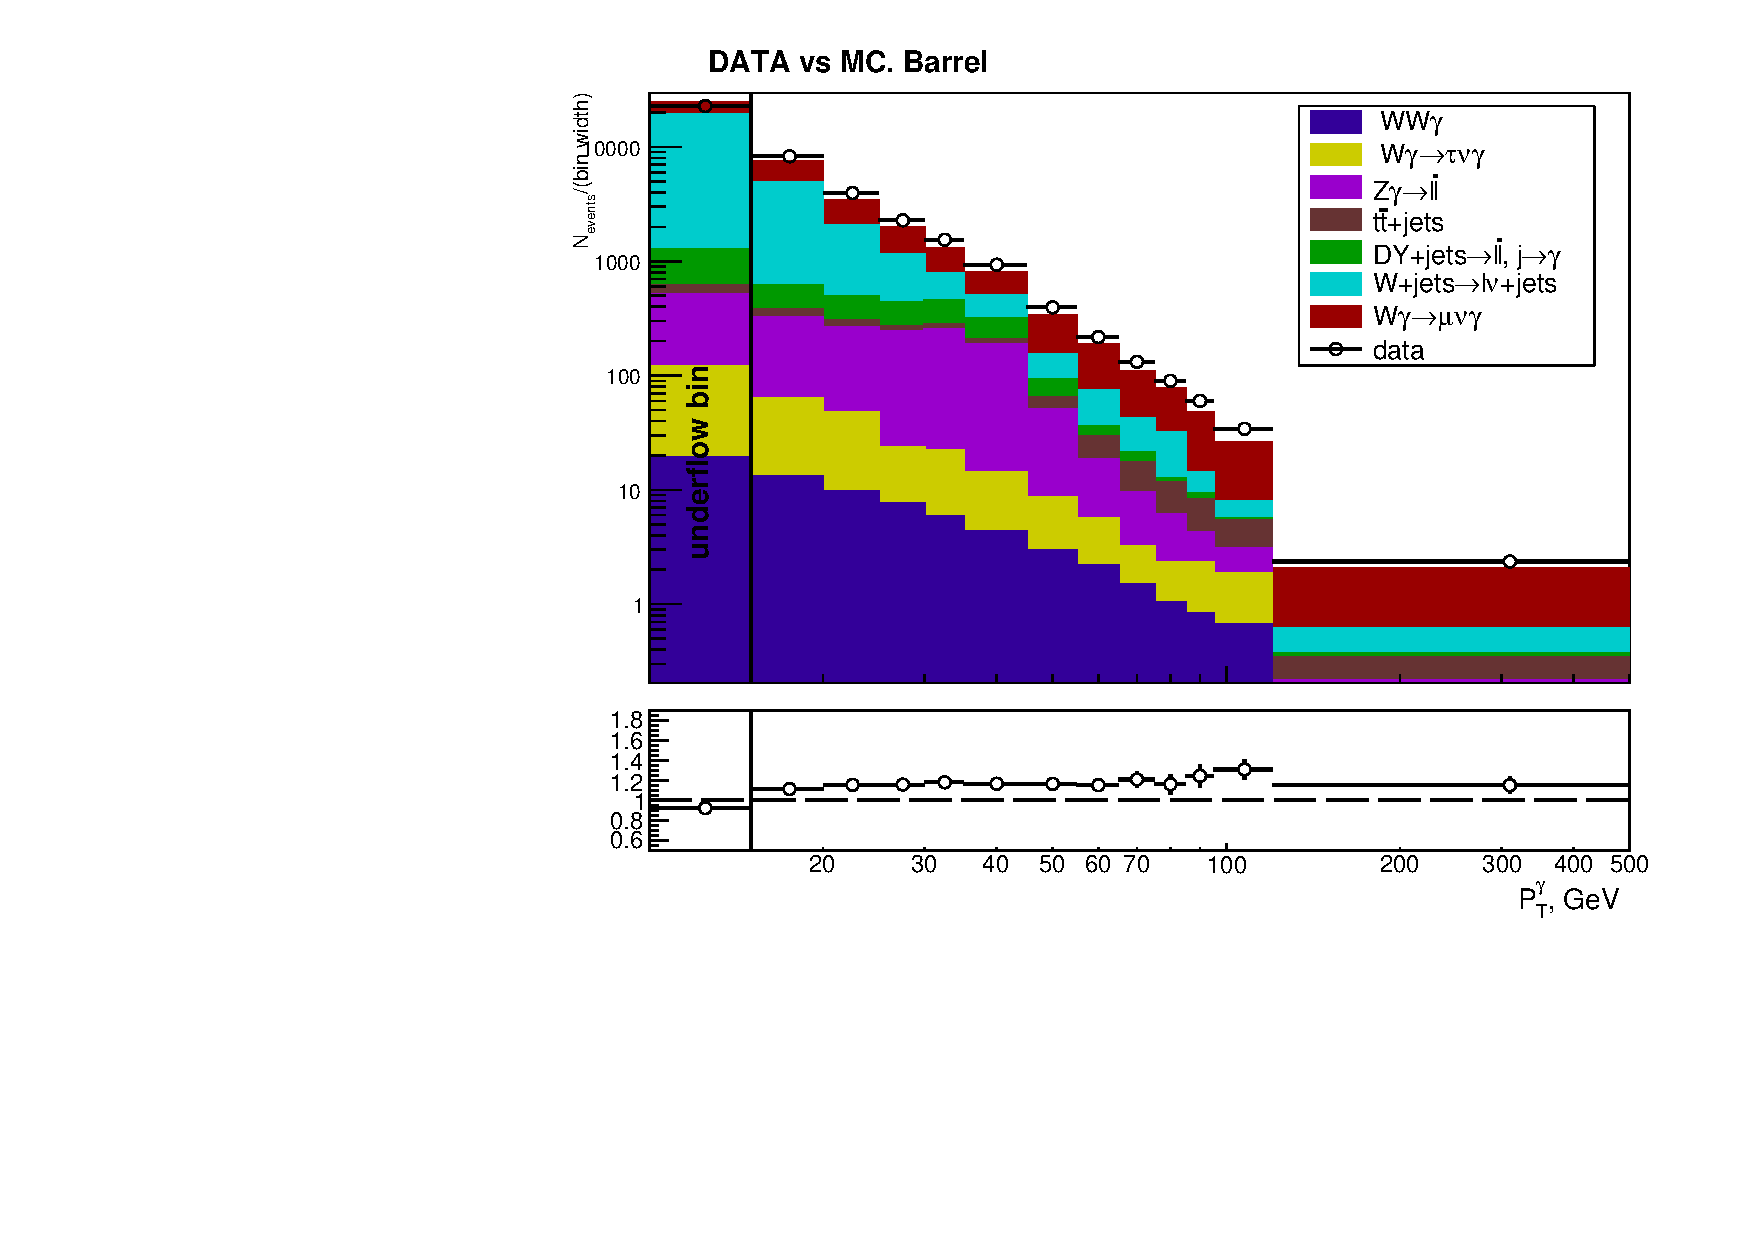
\includegraphics[width=0.49\textwidth]{../figs/figs_v11/MUON_WGamma/PrepareYields/c_TotalDATAvsMC_Barrel__phoEt.pdf} 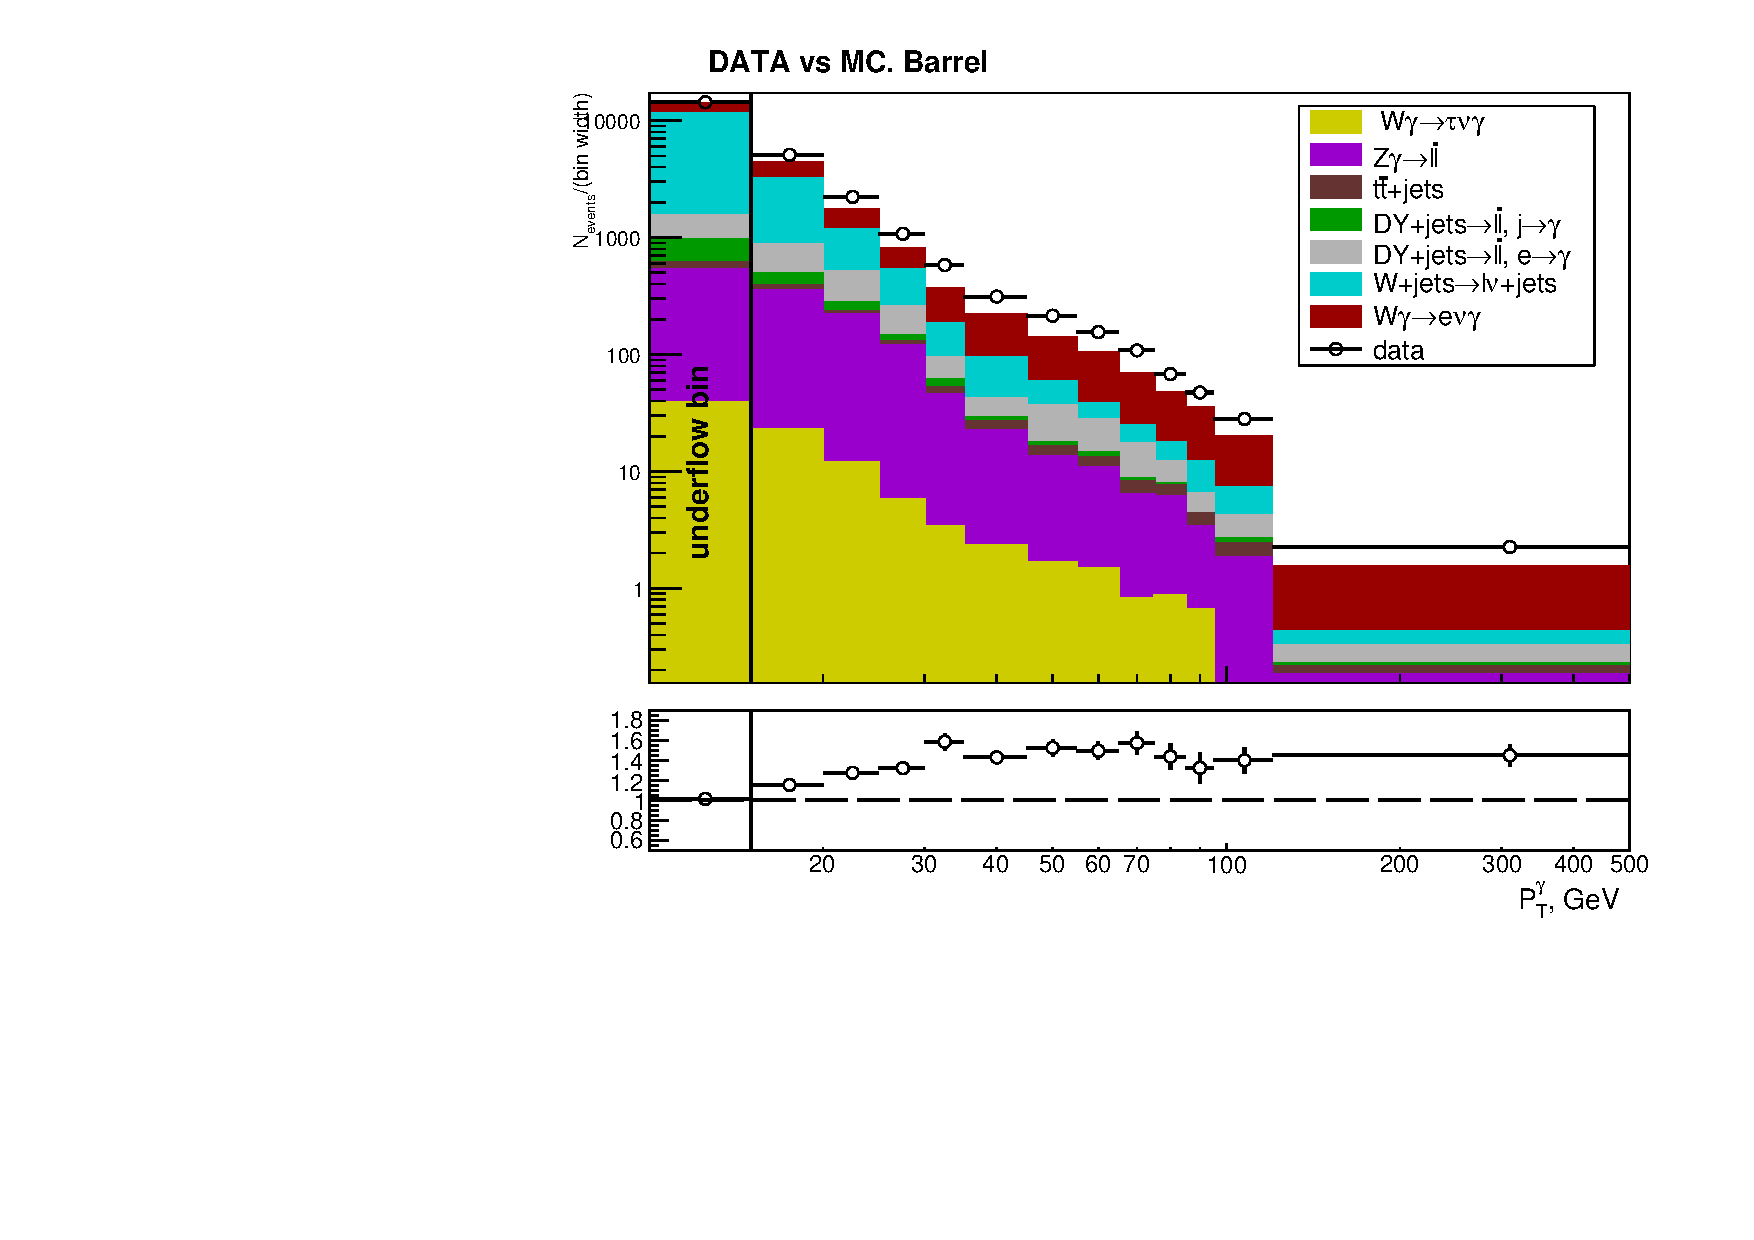
\includegraphics[width=0.49\textwidth]{../figs/figs_v11/ELECTRON_WGamma/PrepareYields/c_TotalDATAvsMC_Barrel__phoEt.pdf} 
    \end{center}
  \end{figure}

\tiny
  \begin{table}[h]
     \tiny
     \begin{center}
     \begin{tabular}{|l|l|}
     \hline
     {\bfseries{Comments:}} &  {\color{white}\bfseries{ Backgrounds:}}\\ 
     Dominated by $W$+jets events in low $P_T^{\gamma}$ bins; &{\color{white}Jets$\rightarrow\gamma$: $W$+jets, DY+jets, $t\bar{t}$+jets;}\\
     Fraction of signal increases with $P_T^{\gamma}$; & {\color{white}$e\rightarrow\gamma$: DY+jets (electron channel only);}\\
     Data disagree with MC.          & {\color{white}real-$\gamma$: $Z\gamma$, $W\gamma\rightarrow\tau\nu\gamma$.}\\
     \hline
      \end{tabular}
      \end{center}
  \end{table}

\end{frame}


\begin{frame}\frametitle{$P_T^{\gamma}$ Spectrum of $W\gamma$ Candidates}
  \begin{figure}[htb]
    \begin{center}
       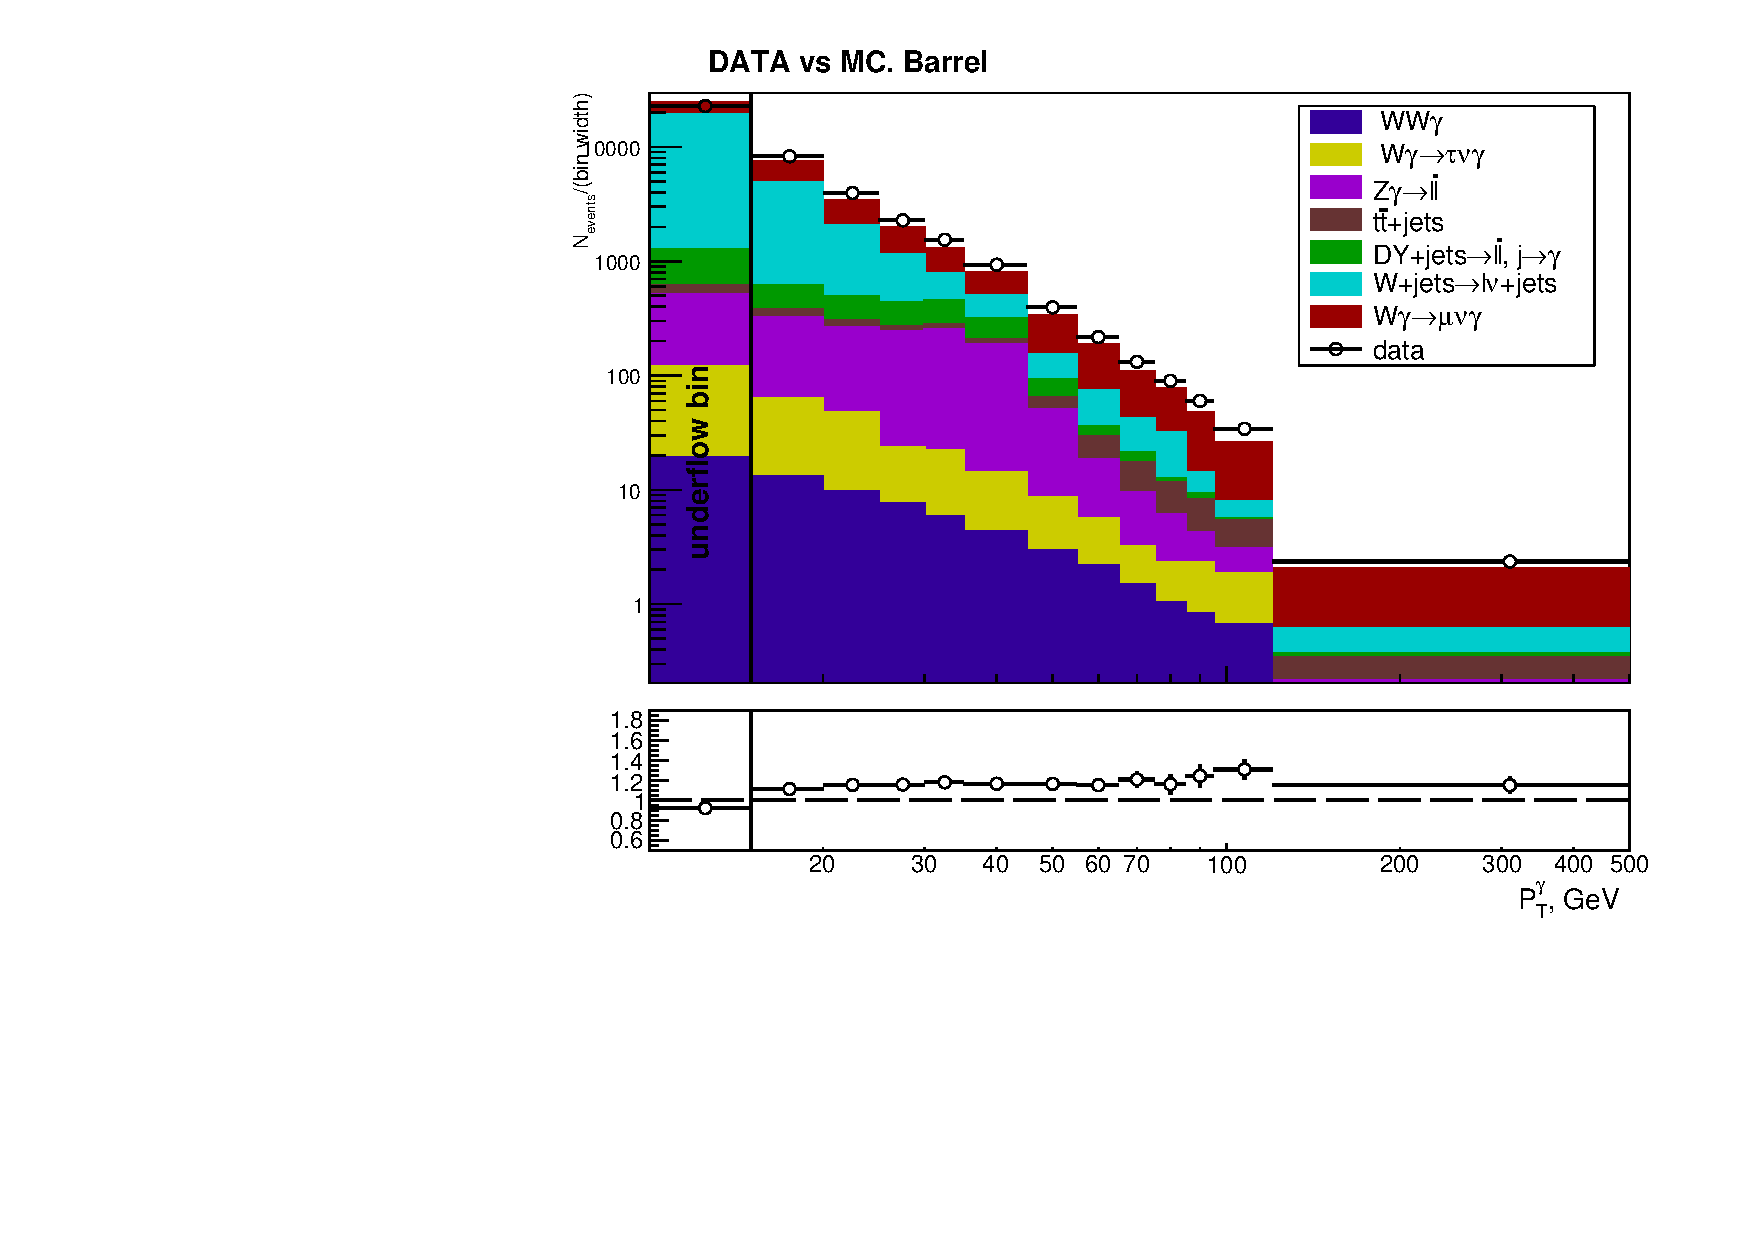
\includegraphics[width=0.49\textwidth]{../figs/figs_v11/MUON_WGamma/PrepareYields/c_TotalDATAvsMC_Barrel__phoEt.pdf} 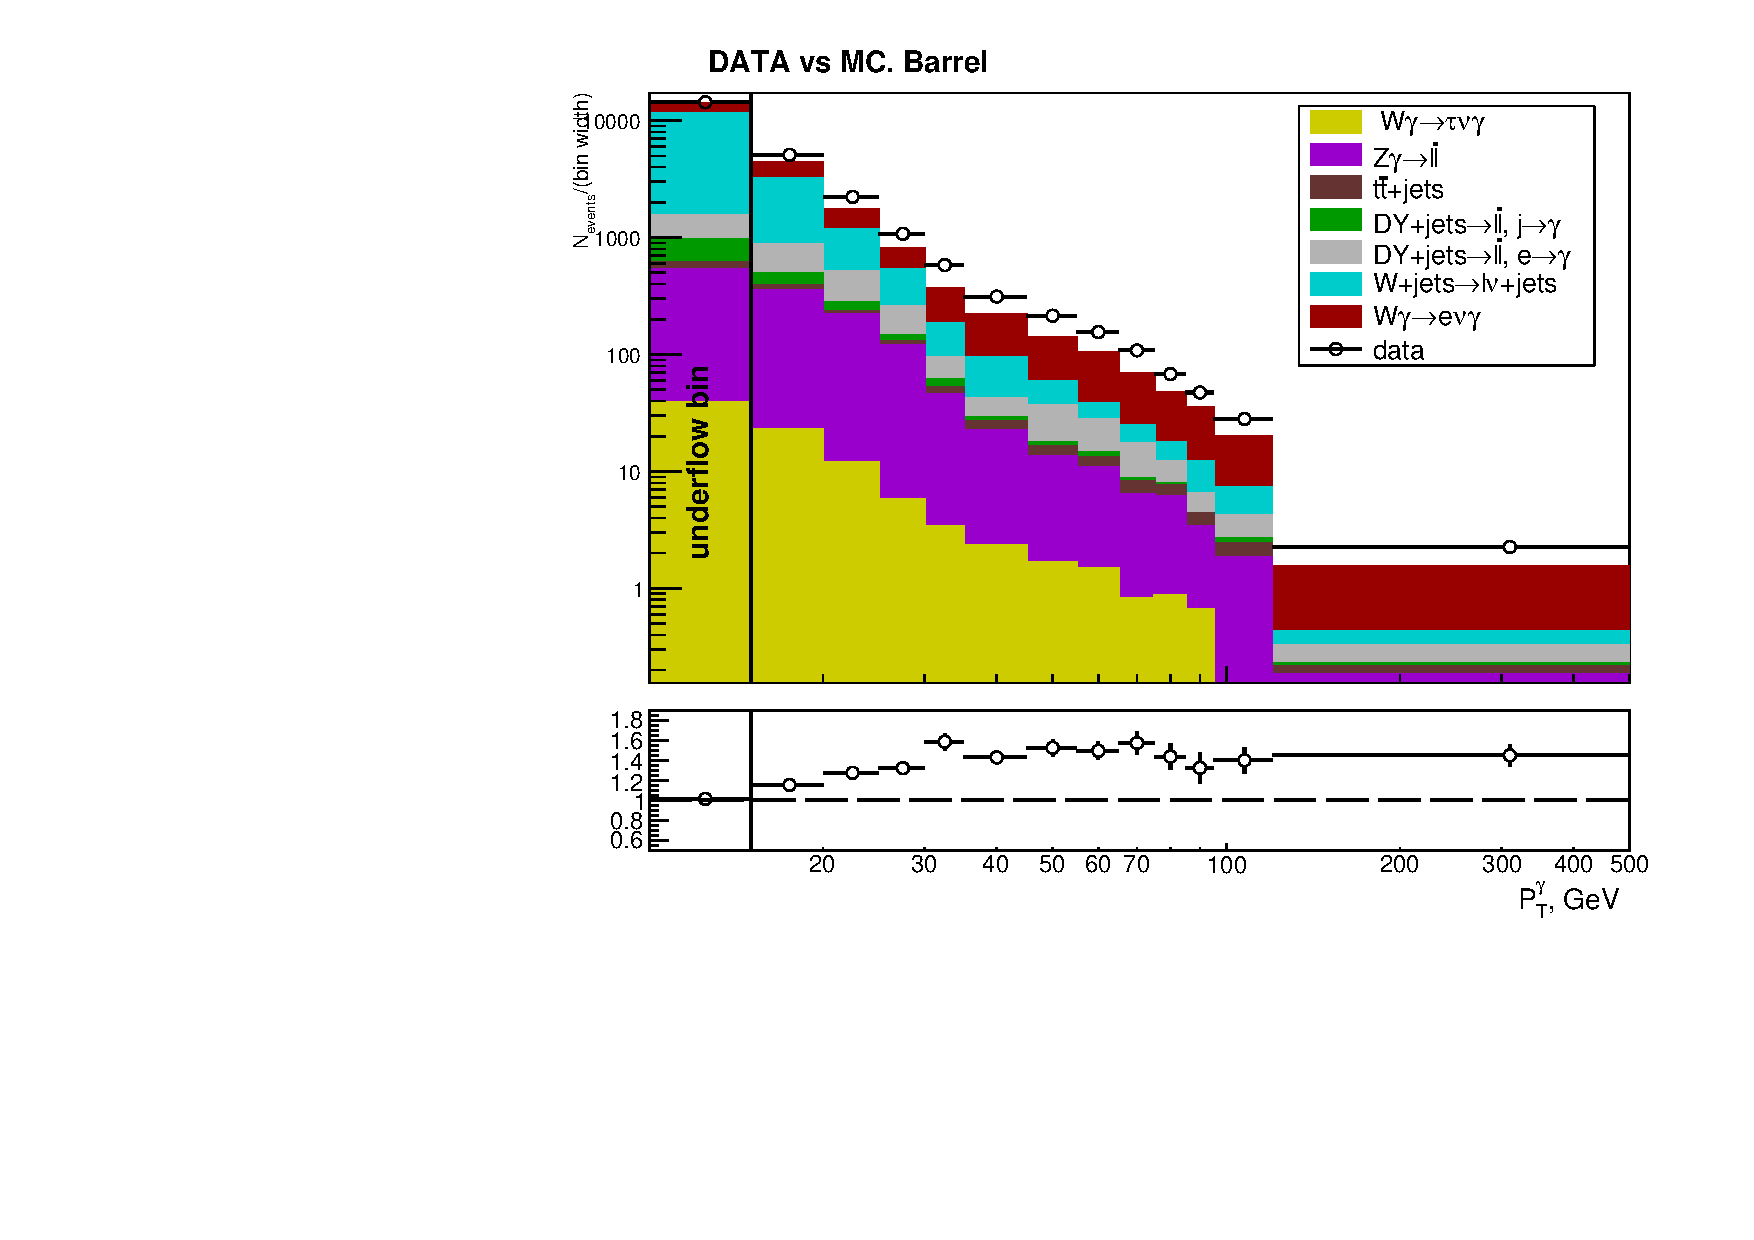
\includegraphics[width=0.49\textwidth]{../figs/figs_v11/ELECTRON_WGamma/PrepareYields/c_TotalDATAvsMC_Barrel__phoEt.pdf} 
    \end{center}
  \end{figure}

\tiny
  \begin{table}[h]
     \tiny
     \begin{center}
     \begin{tabular}{|l|l|}
     \hline
     {\color{gray}\bfseries{Comments:}} &  {\bfseries{ Backgrounds:}}\\ 
     {\color{gray}Dominated by $W$+jets events in low $P_T^{\gamma}$ bins;} & Jets$\rightarrow\gamma$: $W$+jets, DY+jets, $t\bar{t}$+jets;\\
     {\color{gray}Fraction of signal increases with $P_T^{\gamma}$;} & $e\rightarrow\gamma$: DY+jets (electron channel only);\\
     {\color{gray}Data disagree with MC. }         & Real-$\gamma$: $Z\gamma$, $W\gamma\rightarrow\tau\nu\gamma$.\\
     \hline
      \end{tabular}
      \end{center}
  \end{table}

\end{frame}


 % selection, WMt, Mlg, Pt_gamma plots
\begin{frame}\frametitle{Jets$\rightarrow \gamma$ Background. Sources}
  \scriptsize
  \begin{itemize}
    \item Fit function: $F(V_{fit})=N_{true} \cdot T_{true}(V_{fit}) + N_{fake} \cdot T_{fake}(V_{fit})$
%    \item $V_{fit}=I_{ch}^{\gamma}$ and $V_{fit}=\sigma_{i\eta{i\eta}}$ are considered
%    \item $T_{true}$: Real-$\gamma$ template from Z$\gamma\rightarrow\mu\mu\gamma$ FSR minus [small] fake contamination based on DYjets MC
%    \item $T_{fake}$: Fake-$\gamma$ template from Z$\gamma\rightarrow\mu\mu\gamma$ ISR minus [large] real contamination based on Z$\gamma$ MC
%    \item For $I_{ch}$, real-$\gamma$: use full data $p_T^{\gamma}>15~GeV$, fake-$\gamma$: use data only for certain $p_T^{\gamma}$ to prepare template;
%    \item For $\sigma_{i\eta{i\eta}}$, real-$\gamma$: merge data for $p_T^{\gamma}>30~GeV$ for preparing templates, fake-$\gamma$: merge data for $p_T^{\gamma}>55~GeV$;
%    \item Same templates for the muon and the electron channels;
%    \item Algorithm of template rebinning is applied if necessary;
%    \item After fit is performed, extract $N_{real}=\epsilon_{real} \cdot N_{real}^{from-fit}$,  $N_{fake}=\epsilon_{fake} \cdot N_{fake}^{from-fit}$, where $\epsilon_{real}$($\epsilon_{fake}$) is efficiency of real-$\gamma$(fake-$\gamma$) events to pass the nominal cut of $V_{fit}$ computed from the Z$\gamma$ FSR sample (Z$\gamma$ ISR data and MC samples).
  \end{itemize}
  \tiny
  Jets$\rightarrow \gamma$ background estimation is the most challenging part of this measurement and also the source of the largest systematic uncertainties (discussed lated).
\end{frame}

\begin{frame}\frametitle{Jets$\rightarrow \gamma$ Background. General Description of the Template Method}
  \scriptsize
  \begin{itemize}
    \item Fit function: $F(V_{fit})=N_{true} \cdot T_{true}(V_{fit}) + N_{fake} \cdot T_{fake}(V_{fit})$
%    \item $V_{fit}=I_{ch}^{\gamma}$ and $V_{fit}=\sigma_{i\eta{i\eta}}$ are considered
%    \item $T_{true}$: Real-$\gamma$ template from Z$\gamma\rightarrow\mu\mu\gamma$ FSR minus [small] fake contamination based on DYjets MC
%    \item $T_{fake}$: Fake-$\gamma$ template from Z$\gamma\rightarrow\mu\mu\gamma$ ISR minus [large] real contamination based on Z$\gamma$ MC
%    \item For $I_{ch}$, real-$\gamma$: use full data $p_T^{\gamma}>15~GeV$, fake-$\gamma$: use data only for certain $p_T^{\gamma}$ to prepare template;
%    \item For $\sigma_{i\eta{i\eta}}$, real-$\gamma$: merge data for $p_T^{\gamma}>30~GeV$ for preparing templates, fake-$\gamma$: merge data for $p_T^{\gamma}>55~GeV$;
%    \item Same templates for the muon and the electron channels;
%    \item Algorithm of template rebinning is applied if necessary;
%    \item After fit is performed, extract $N_{real}=\epsilon_{real} \cdot N_{real}^{from-fit}$,  $N_{fake}=\epsilon_{fake} \cdot N_{fake}^{from-fit}$, where $\epsilon_{real}$($\epsilon_{fake}$) is efficiency of real-$\gamma$(fake-$\gamma$) events to pass the nominal cut of $V_{fit}$ computed from the Z$\gamma$ FSR sample (Z$\gamma$ ISR data and MC samples).
  \end{itemize}
\end{frame}

\begin{frame}\frametitle{Jets$\rightarrow \gamma$ Background. Templates from $Z\gamma\rightarrow{\bar{\mu}}\mu\gamma$, FSR and ISR}
  \begin{figure}[htb]
    \begin{center}
       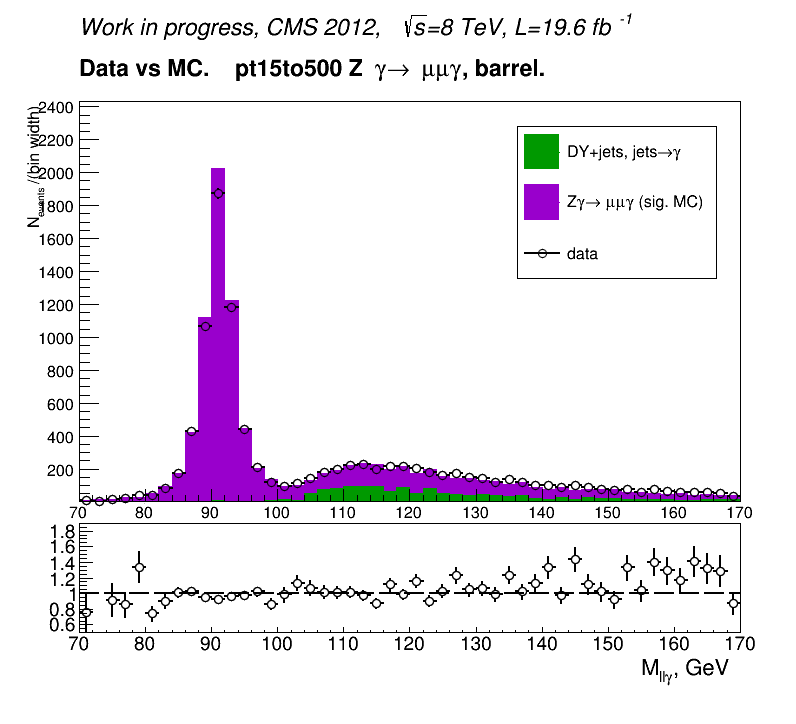
\includegraphics[width=0.45\textwidth]{../figs/figs_v11/MUON_ZGamma/PrepareYields/c_TotalDATAvsMC_Barrel__MpholeplepVERY_PRELIMINARY_pt15to500_.png}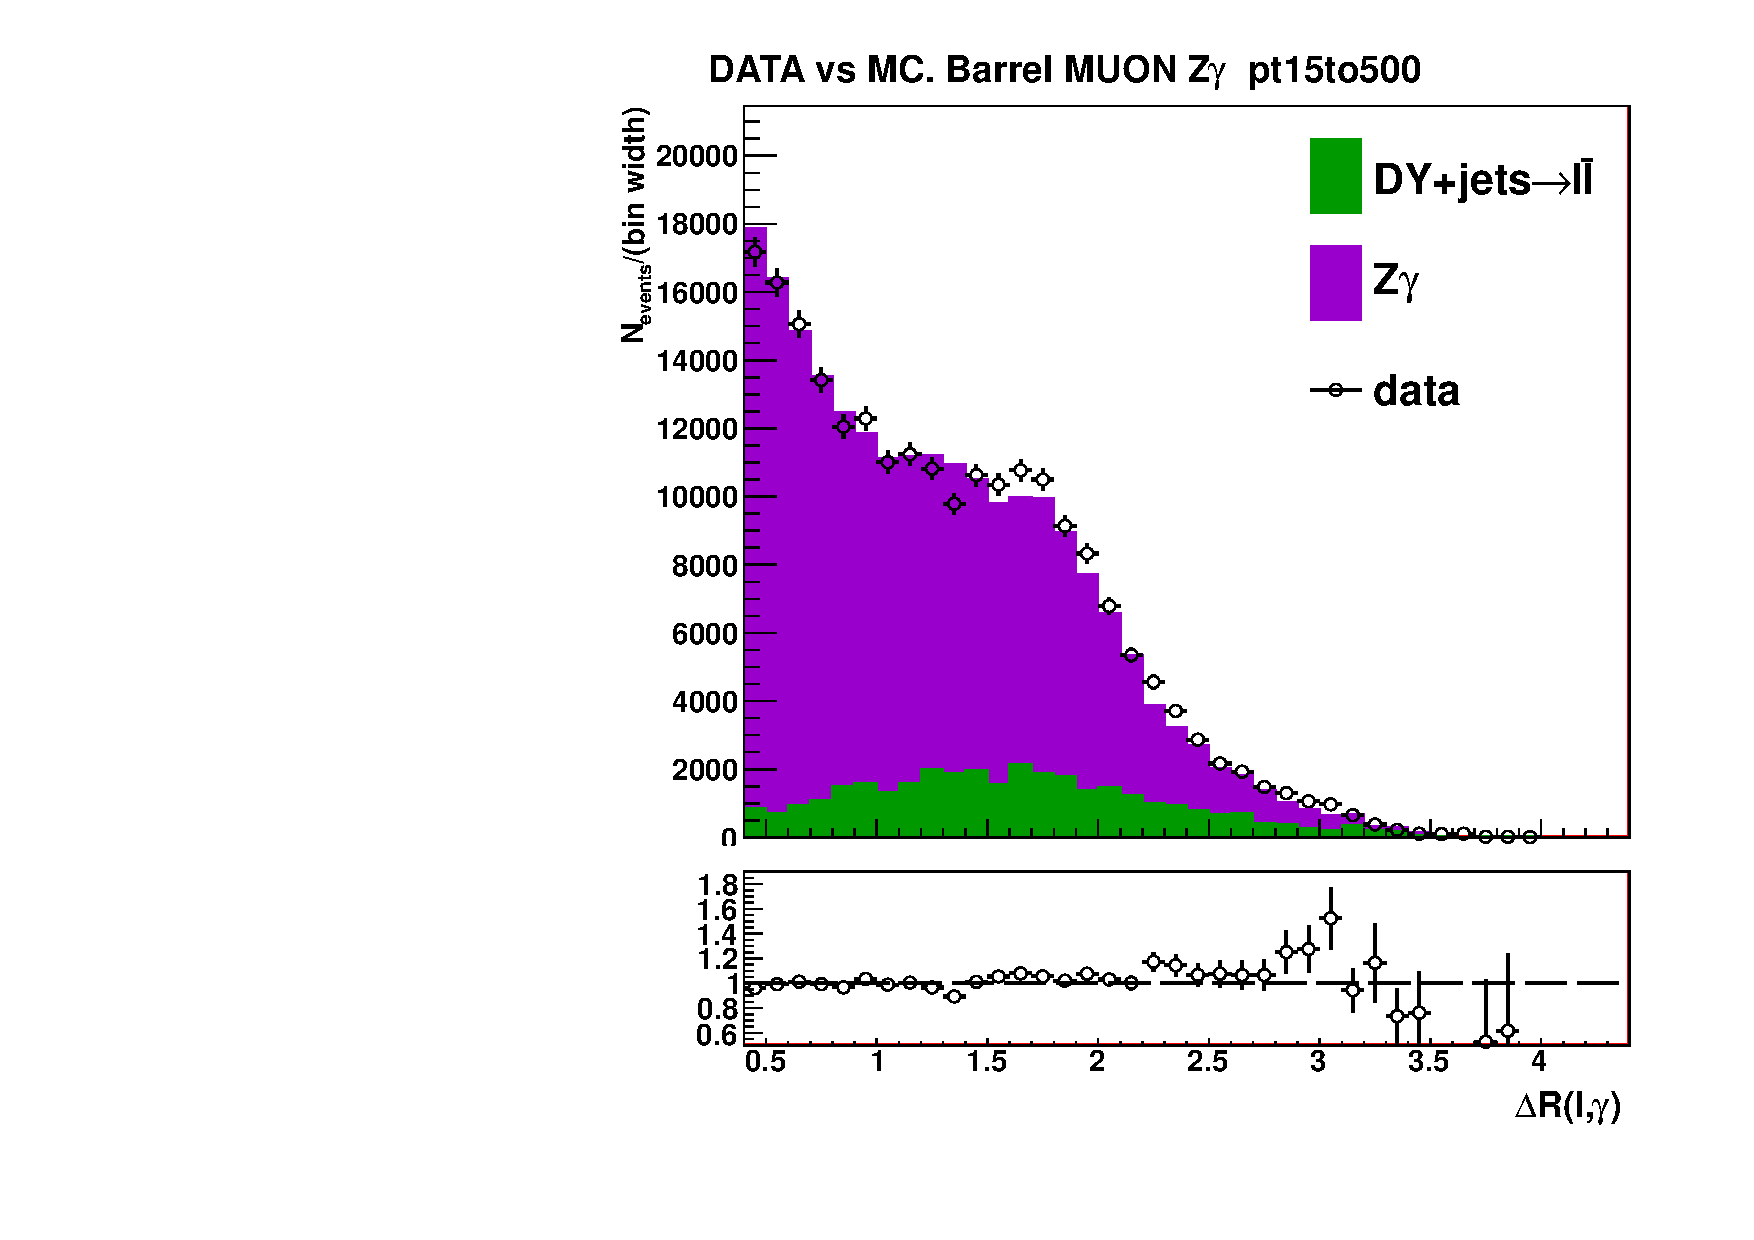
\includegraphics[width=0.45\textwidth]{../figs/figs_v11/MUON_ZGamma/PrepareYields/c_TotalDATAvsMC_Barrel__lep1PhoDeltaRVERY_PRELIMINARY_pt15to500_.pdf}\\
% 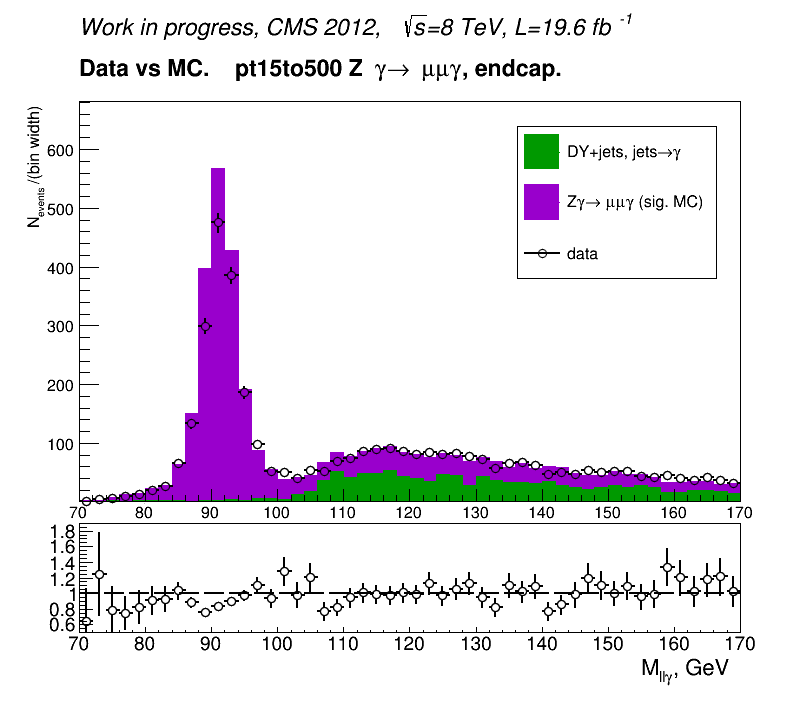
\includegraphics[width=0.40\textwidth]{../figs/figs_v11/MUON_ZGamma/PrepareYields/c_TotalDATAvsMC_Endcap__MpholeplepVERY_PRELIMINARY_pt15to500_.png}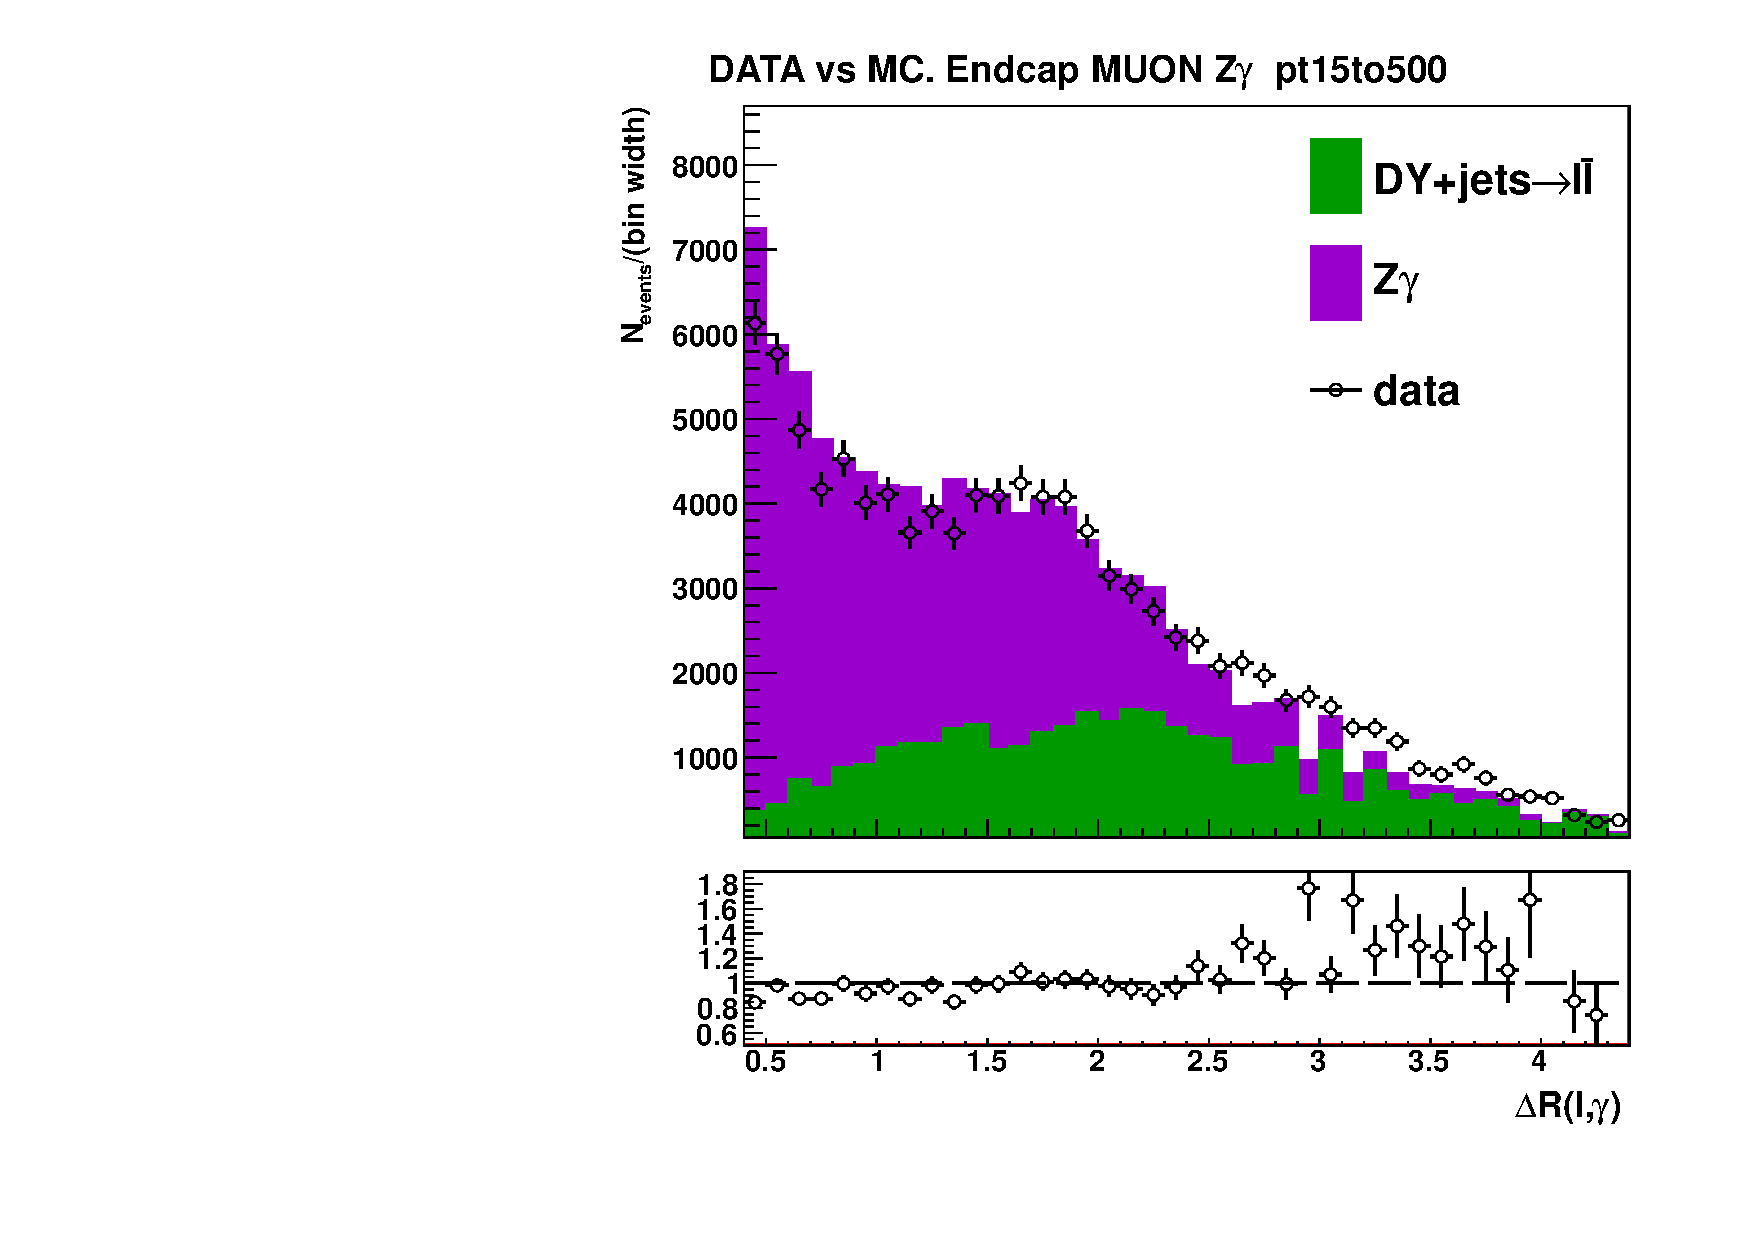
\includegraphics[width=0.40\textwidth]{../figs/figs_v11/MUON_ZGamma/PrepareYields/c_TotalDATAvsMC_Endcap__lep1PhoDeltaRVERY_PRELIMINARY_pt15to500_.pdf}
    \end{center}
  \end{figure}
\scriptize
FSR selection: $M_{\mu\mu\gamma}<101$~GeV and $\Delta R(\mu_{1},\gamma)>0.4$, nominal $Z\gamma$ selection otherwise\\
ISR selection: $M_{\mu\mu\gamma}>101$~GeV and $\Delta R(\mu_{1},\gamma)>1.0$, nominal $Z\gamma$ selection otherwise
\end{frame}%{Z$\gamma$ normalization. FSR and ISR}

\begin{frame}\frametitle{$Jets \rightarrow \gamma$ Background. $V_{fit}=I_{ch}^{\gamma}$}
  \begin{figure}[htb]
    \begin{center}
       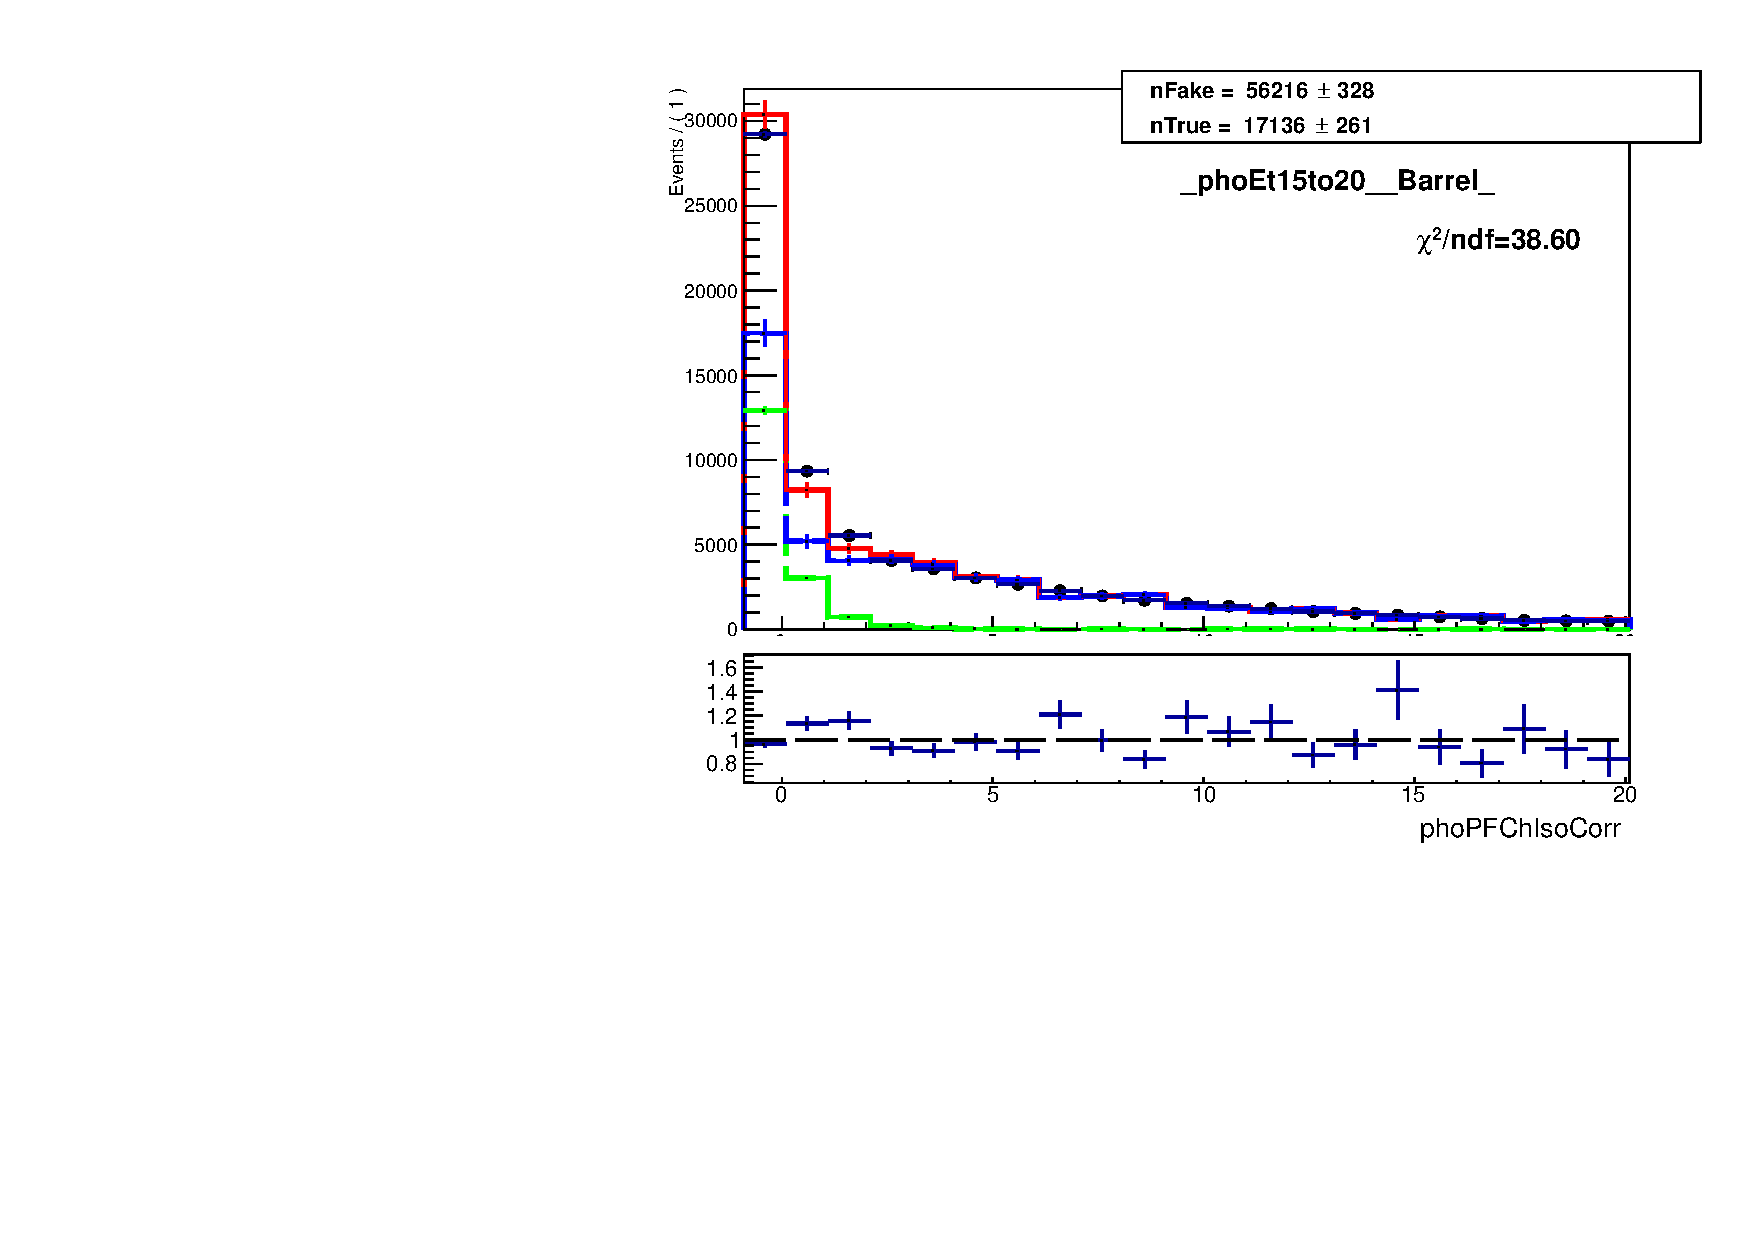
\includegraphics[width=0.45\textwidth]{../figs/figs_v11/MUON_WGamma/TemplateFits/c_TEMPL_CHISO_UNblind__phoEt15to20__Barrel__RooFit.pdf} 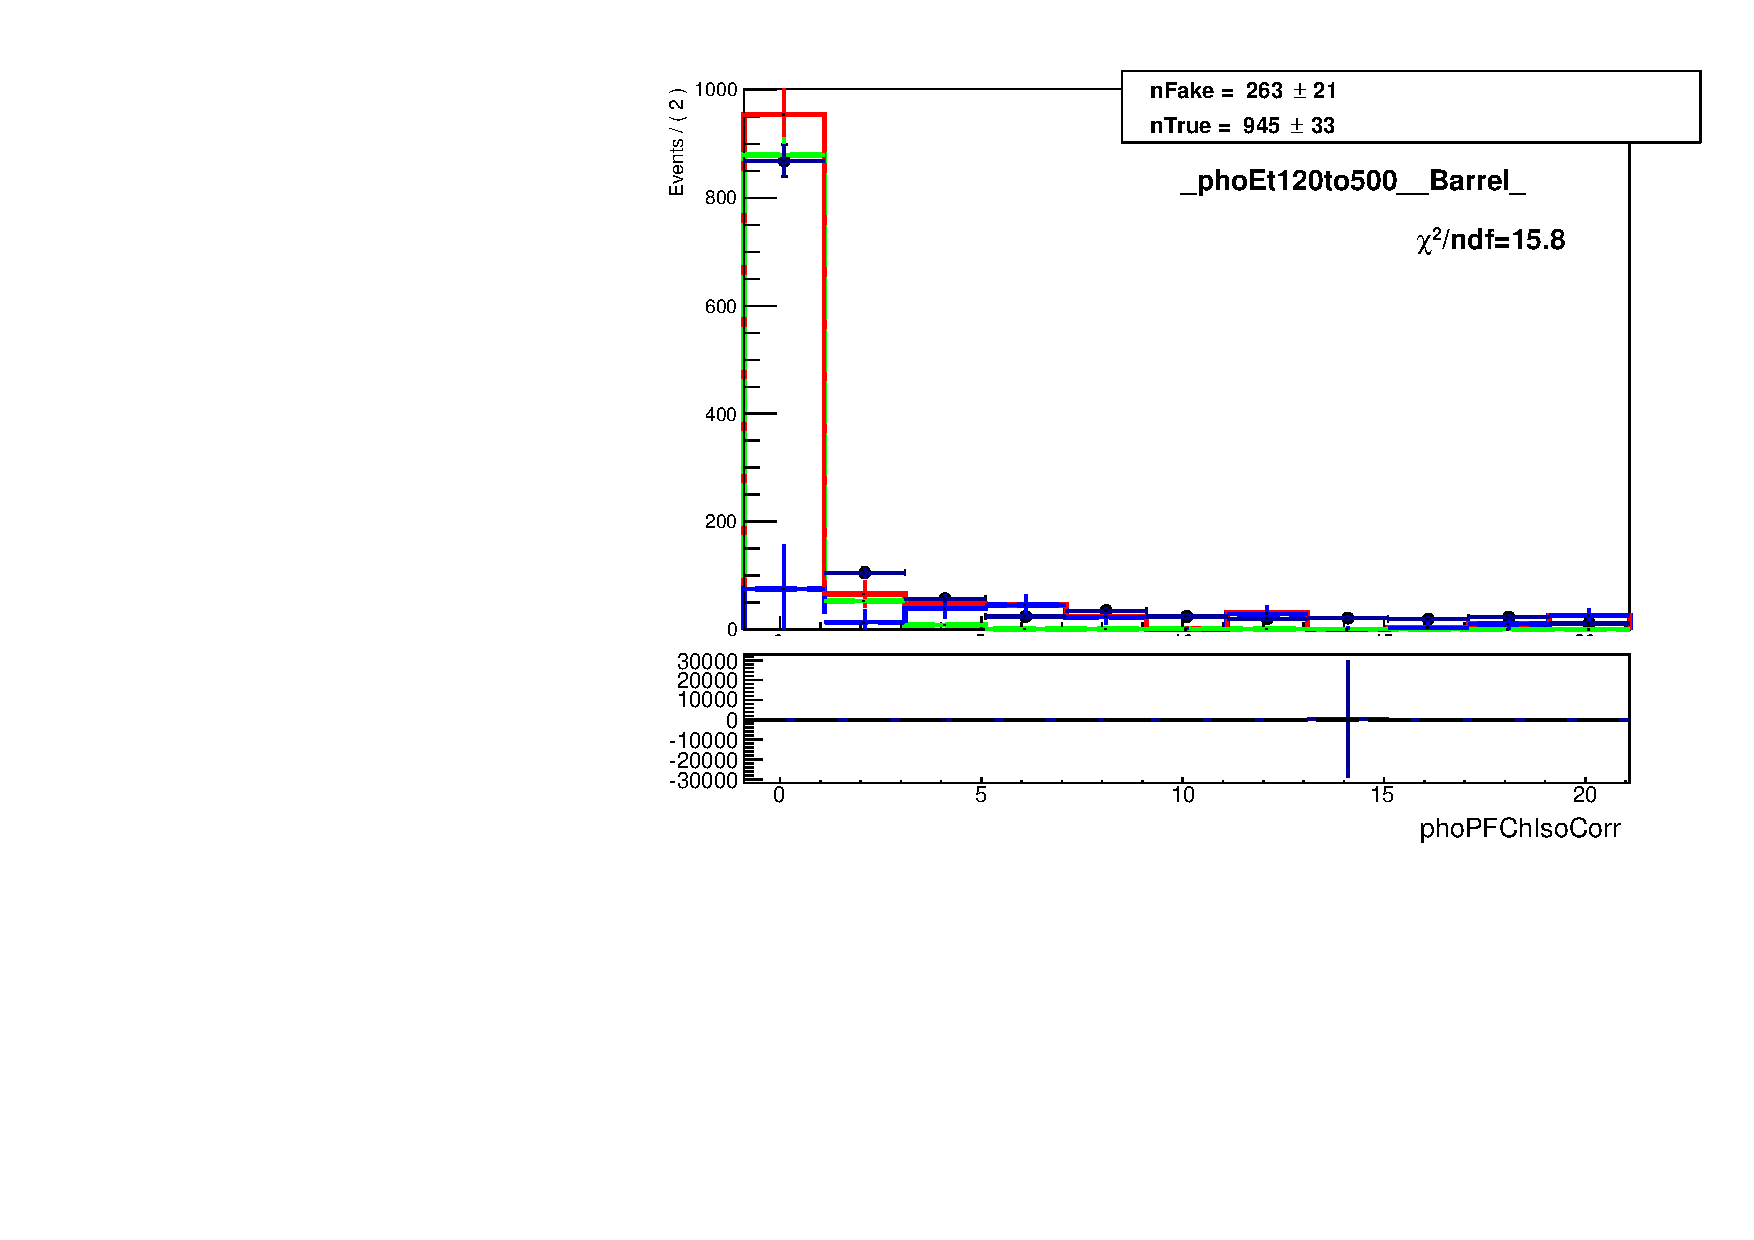
\includegraphics[width=0.45\textwidth]{../figs/figs_v11/MUON_WGamma/TemplateFits/c_TEMPL_CHISO_UNblind__phoEt120to500__Barrel__RooFit.pdf}
    \end{center}
  \end{figure}
\end{frame}%{$Jets \rightarrow \gamma$ Background Subtraction. $V_{fit}=I_{ch}^{\gamma}$}


\begin{frame}\frametitle{$Jets \rightarrow \gamma$ Background. $V_{fit}=\sigma_{i\eta{i\eta}}$}
  \begin{figure}[htb]
    \begin{center}
       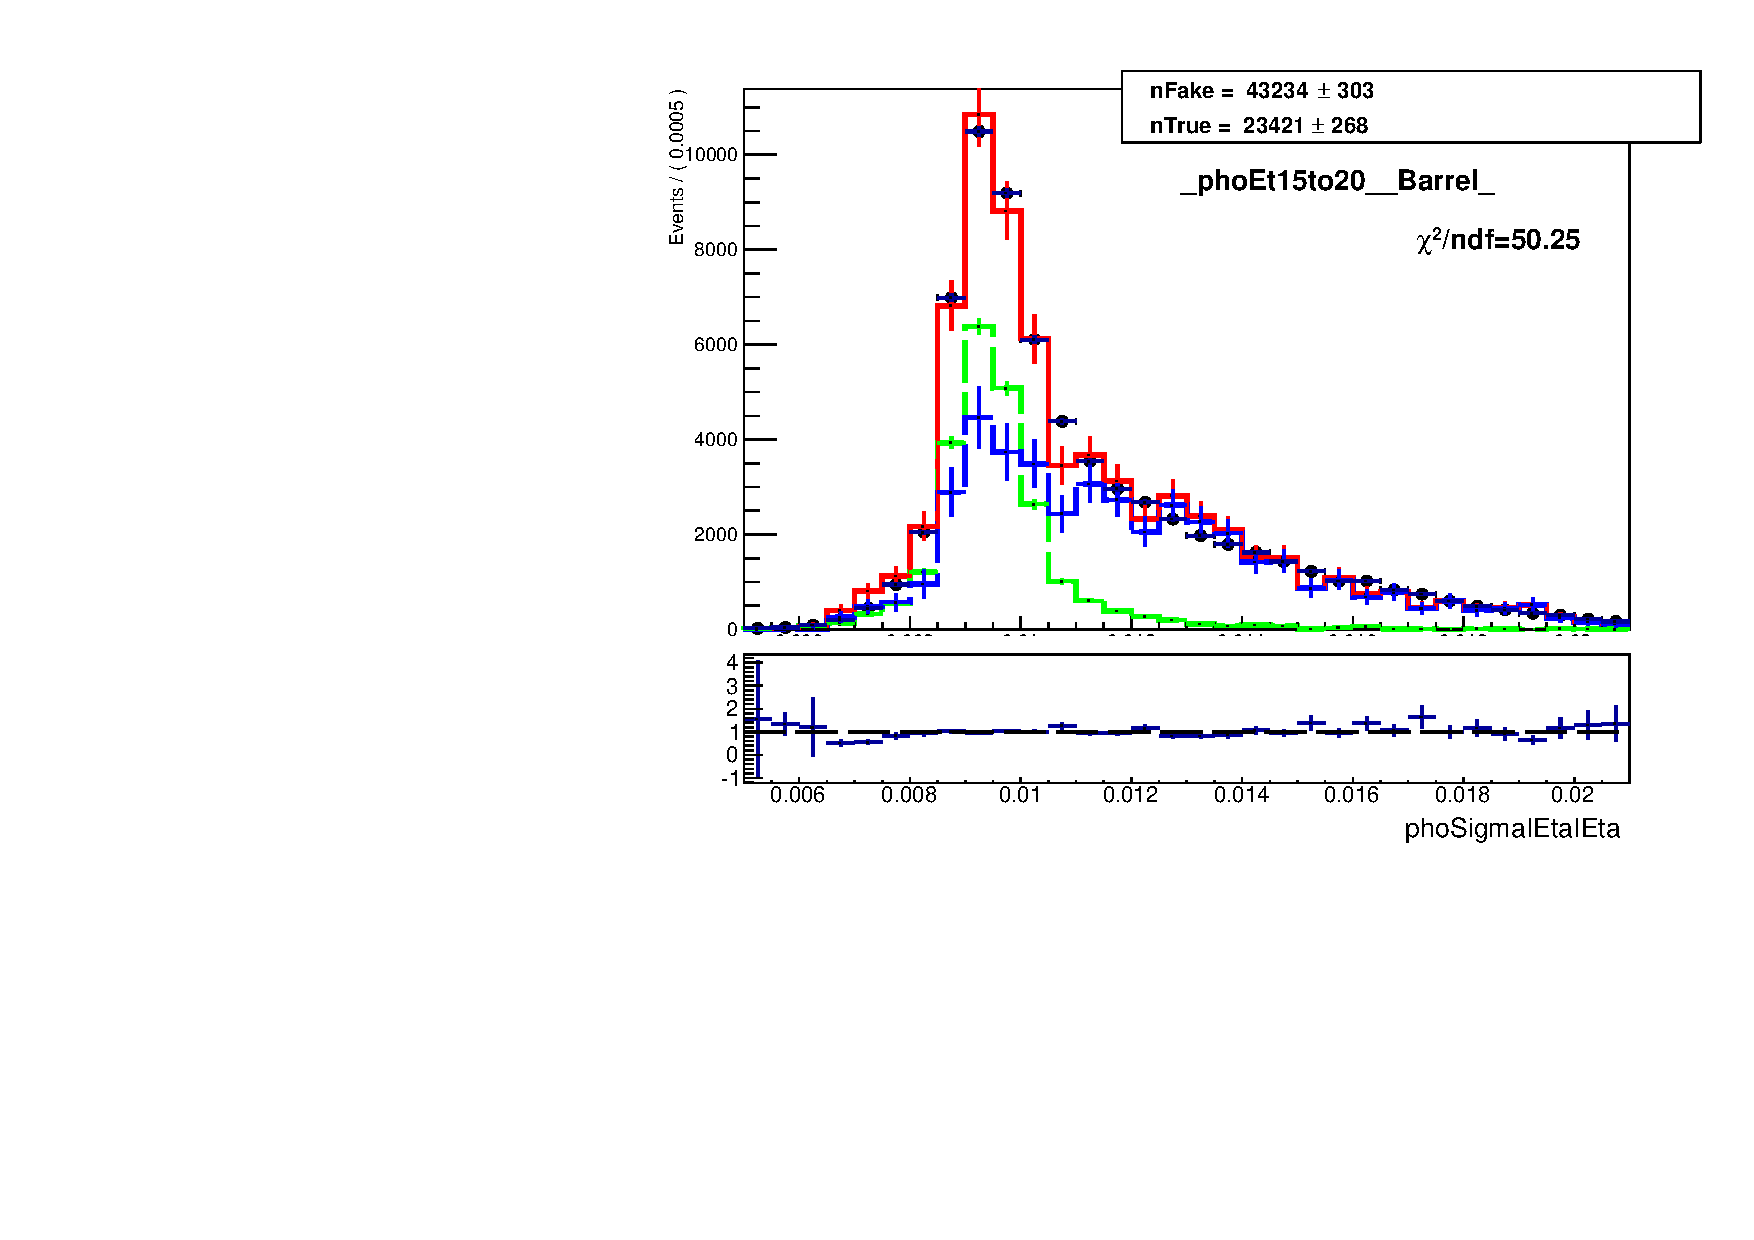
\includegraphics[width=0.45\textwidth]{../figs/figs_v11/MUON_WGamma/TemplateFits/c_TEMPL_SIHIH_UNblind__phoEt15to20__Barrel__RooFit.pdf}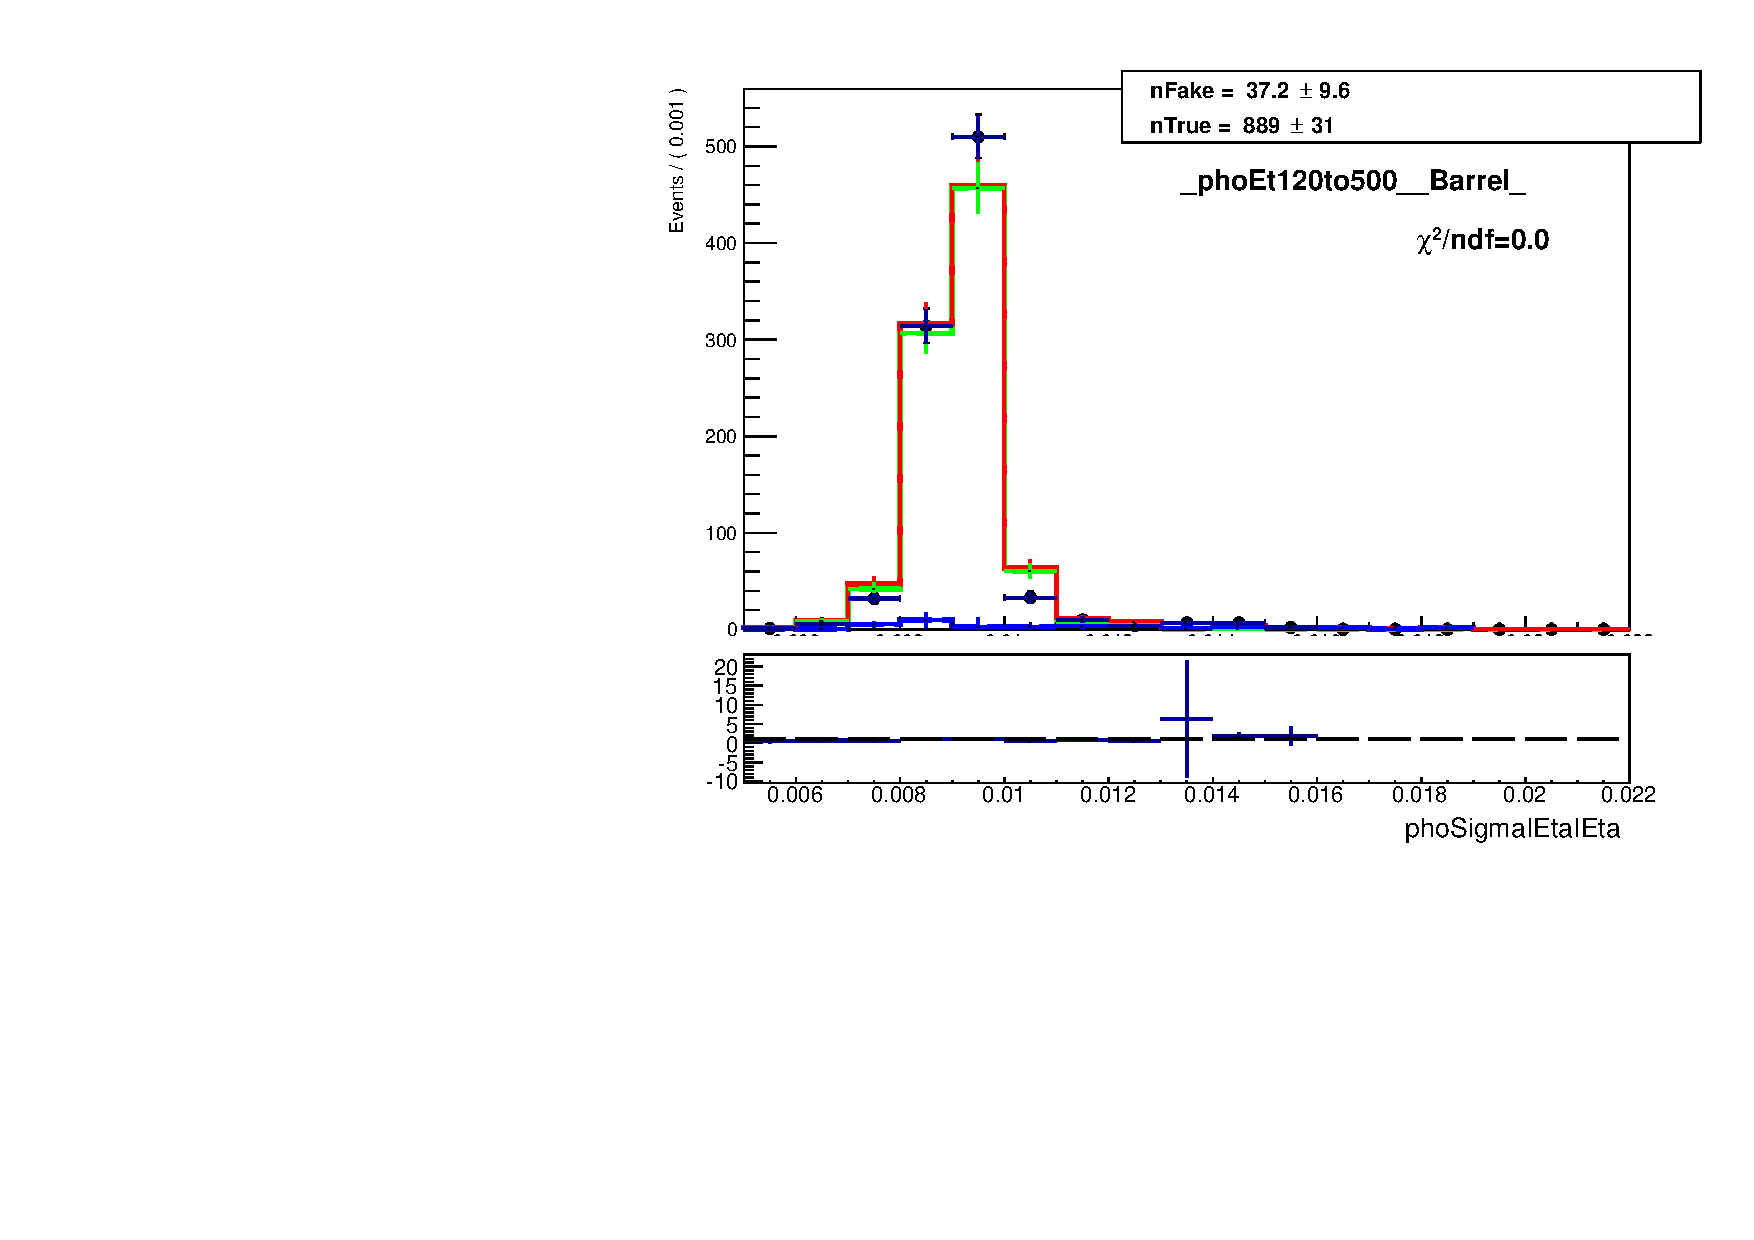
\includegraphics[width=0.45\textwidth]{../figs/figs_v11/MUON_WGamma/TemplateFits/c_TEMPL_SIHIH_UNblind__phoEt120to500__Barrel__RooFit.pdf}
    \end{center}
  \end{figure}
\end{frame}%{$Jets \rightarrow \gamma$ Background Subtraction. $V_{fit}=\sigma_{i\eta{i\eta}}$}
 % method description, FSR and ISR, CHISO, SIHIH
\begin{frame}\frametitle {Real-$\gamma$ Background. Sources}

Main sources of true $\gamma$ background are $Z\gamma$ and $W\gamma \rightarrow \tau \nu \gamma$. The MC-based estimation is used to subtract these backgrounds.

MC-based background estimation.
  \begin{figure}[htb]
    \begin{center}
       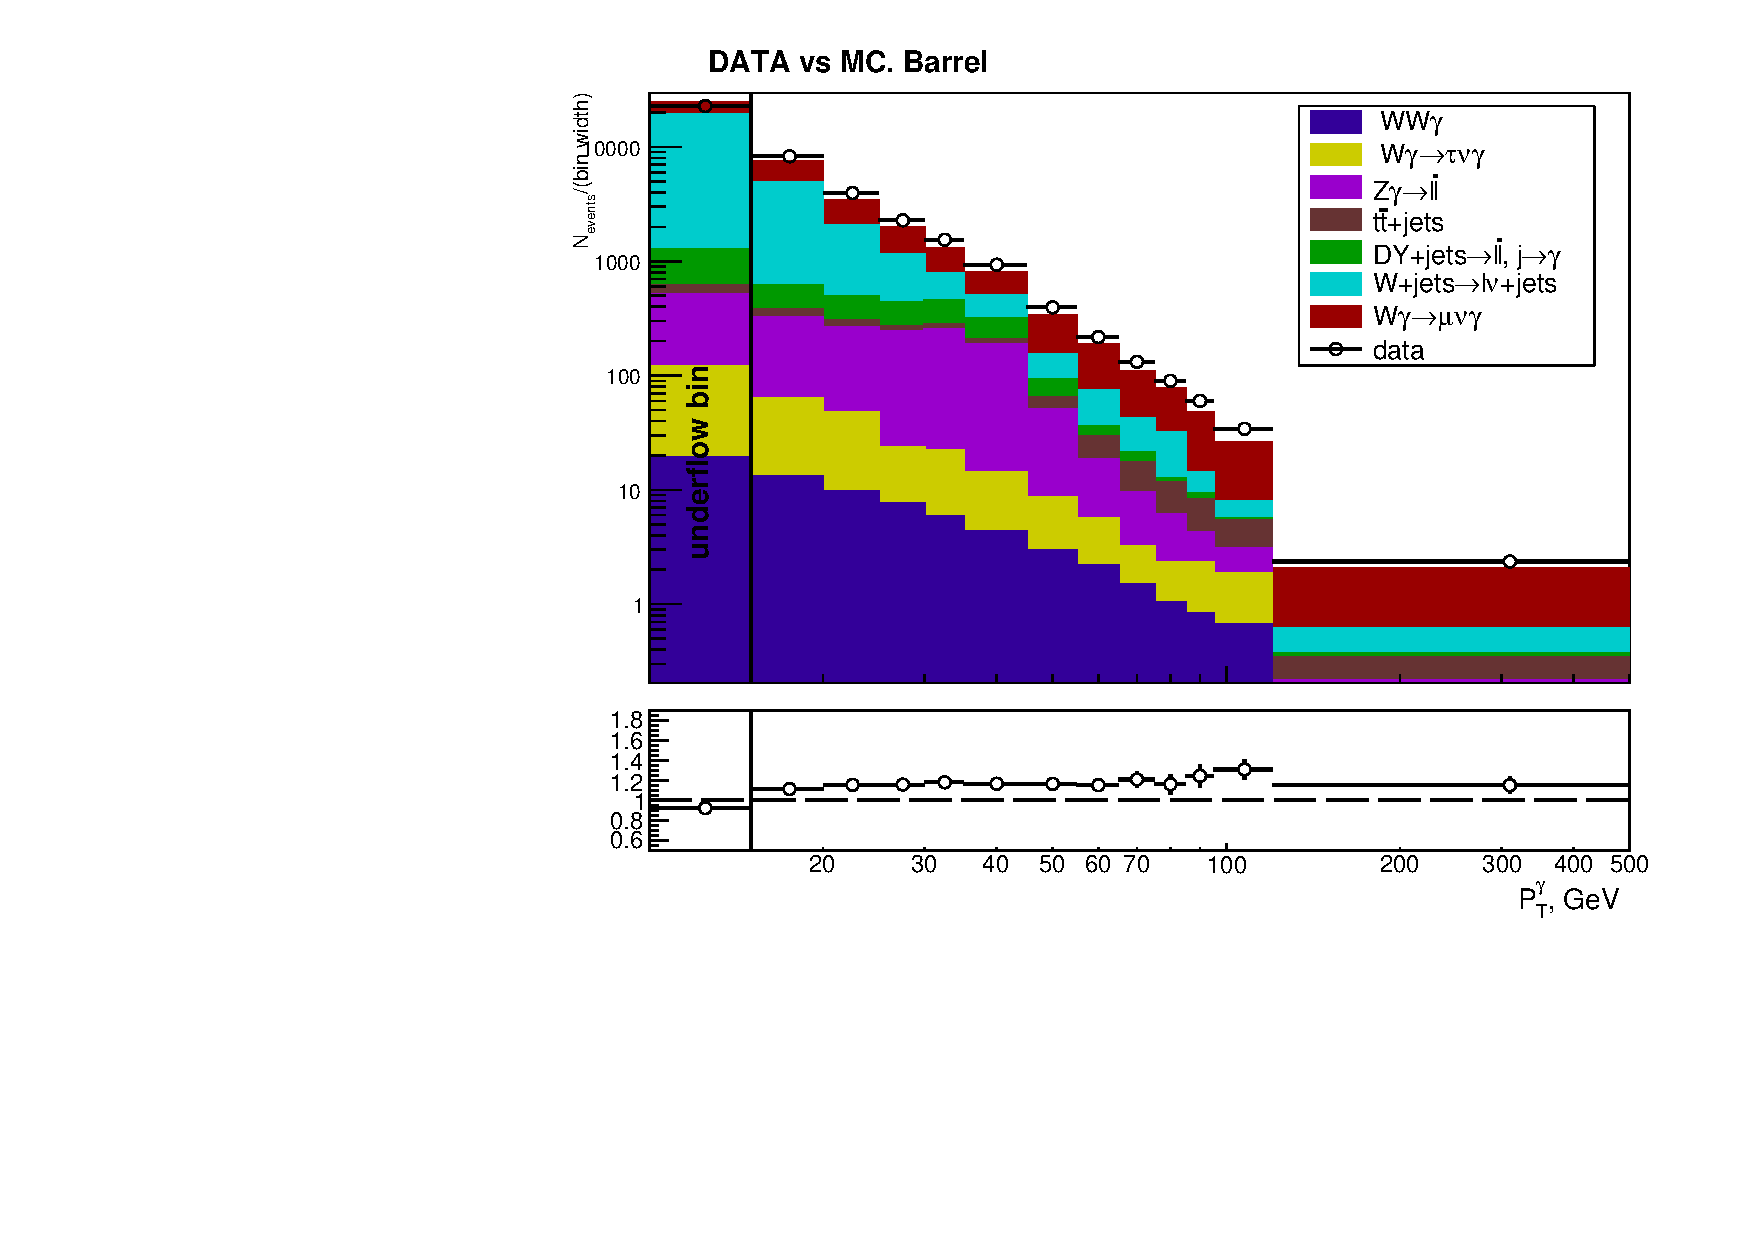
\includegraphics[width=0.40\textwidth]{../figs/figs_v11/MUON_WGamma/PrepareYields/c_TotalDATAvsMC_Barrel__phoEt.pdf}
    \end{center}
  \end{figure}
\end{frame}%{Real-$\gamma$ Backgrounds}

\begin{frame}\frametitle{\footnotesize{$P_T^{\gamma}$ Spectrum (EB only)}}
   \begin{figure}[htb]
    \begin{center}
       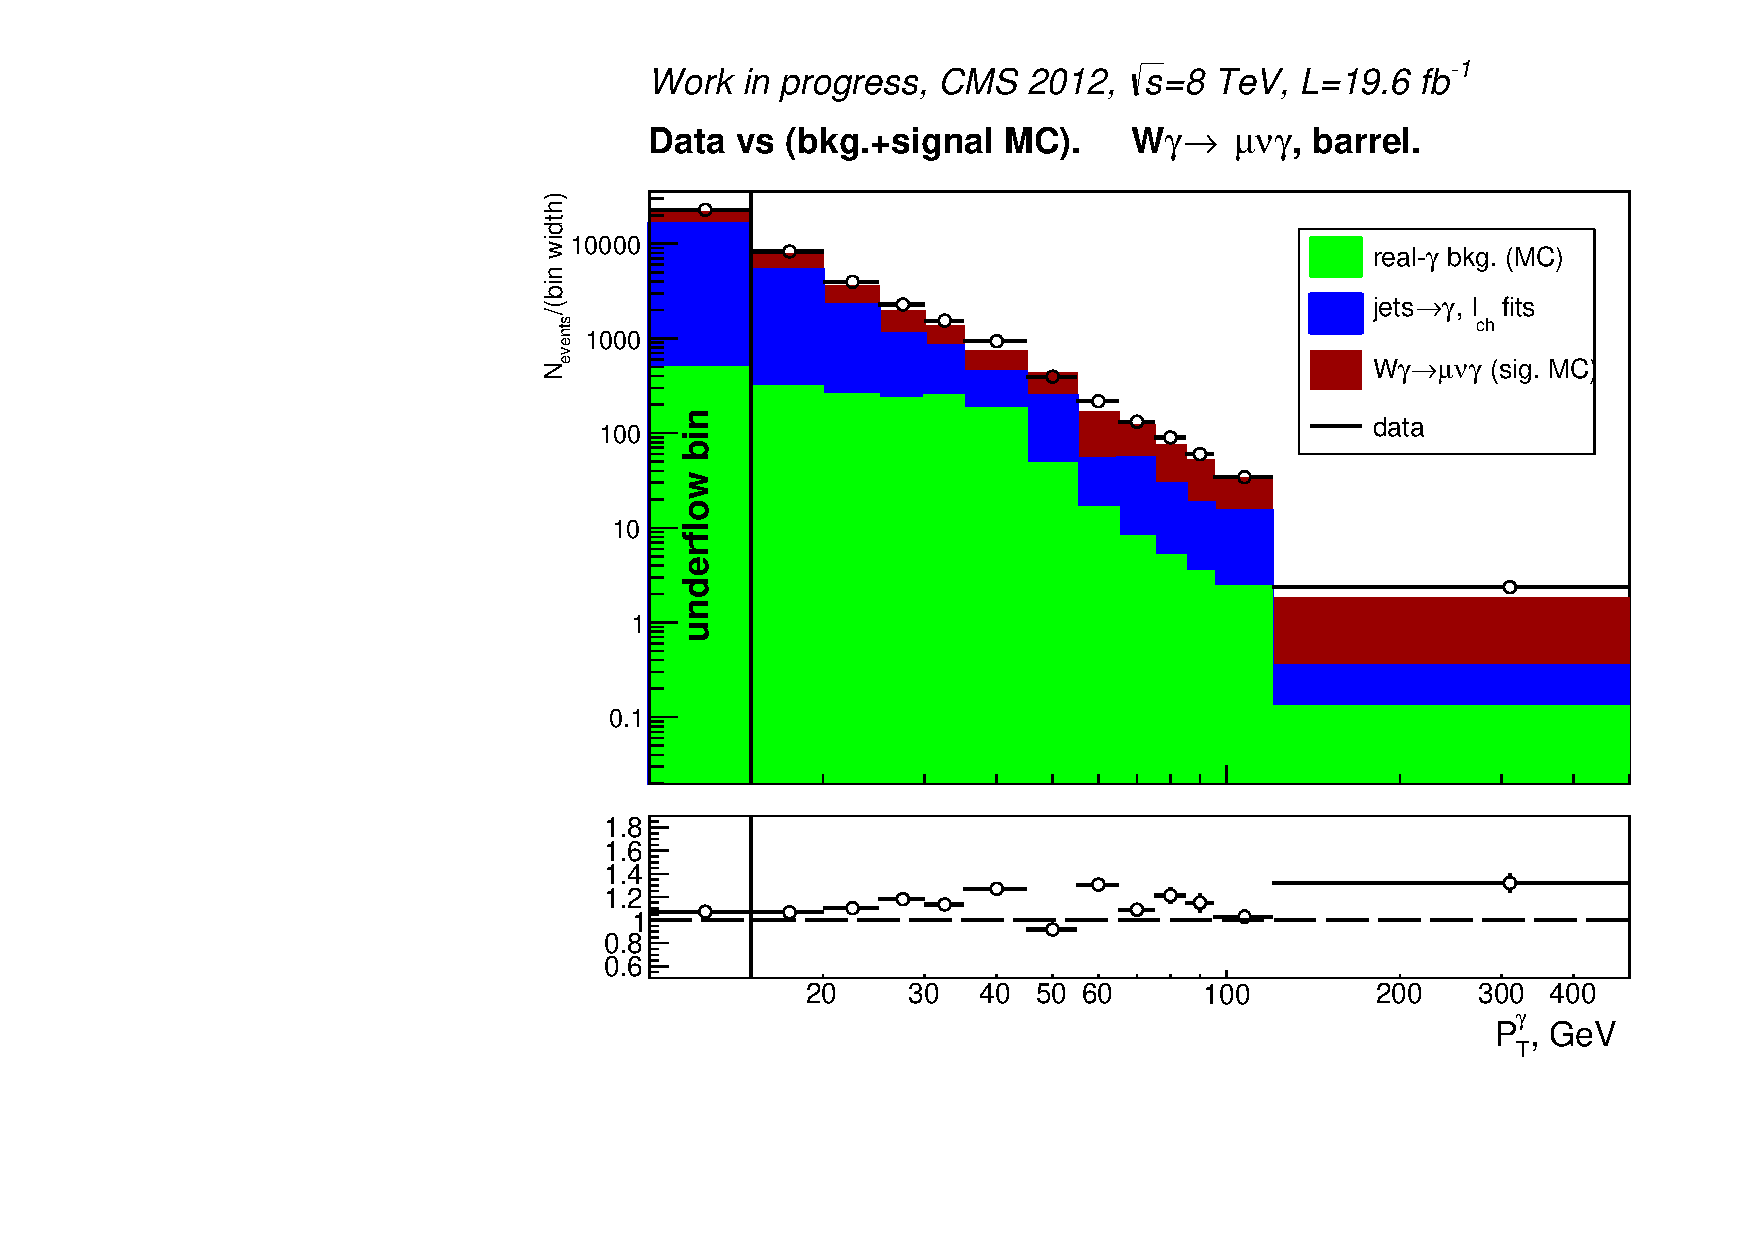
\includegraphics[width=0.40\textwidth]{../figs/figs_v11/MUON_WGamma/PrepareYields/c_DATAvsBkgPlusSigMCc_MUON_WGamma_TEMPL_CHISO_UNblind__Barrel__phoEt.pdf}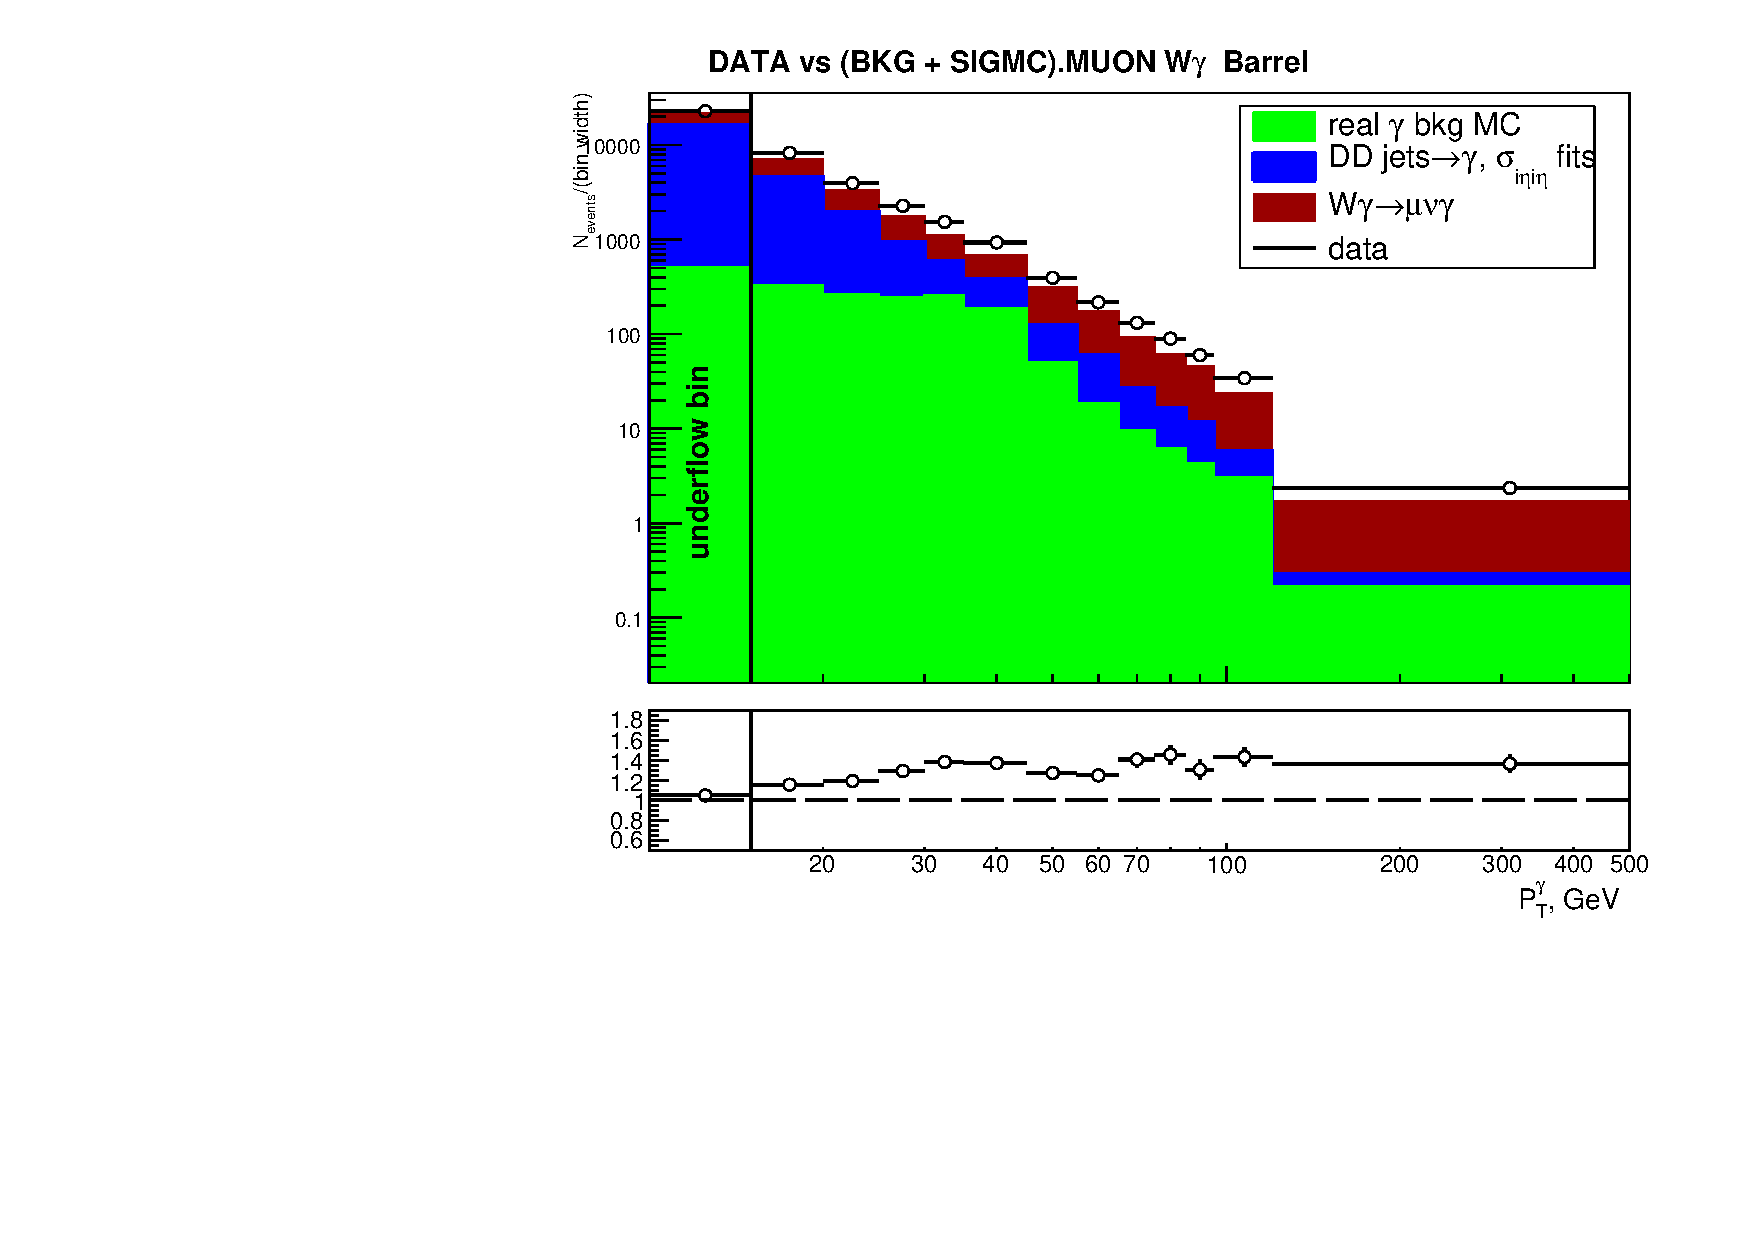
\includegraphics[width=0.40\textwidth]{../figs/figs_v11/MUON_WGamma/PrepareYields/c_DATAvsBkgPlusSigMCc_MUON_WGamma_TEMPL_SIHIH_UNblind__Barrel__phoEt.pdf}\\
       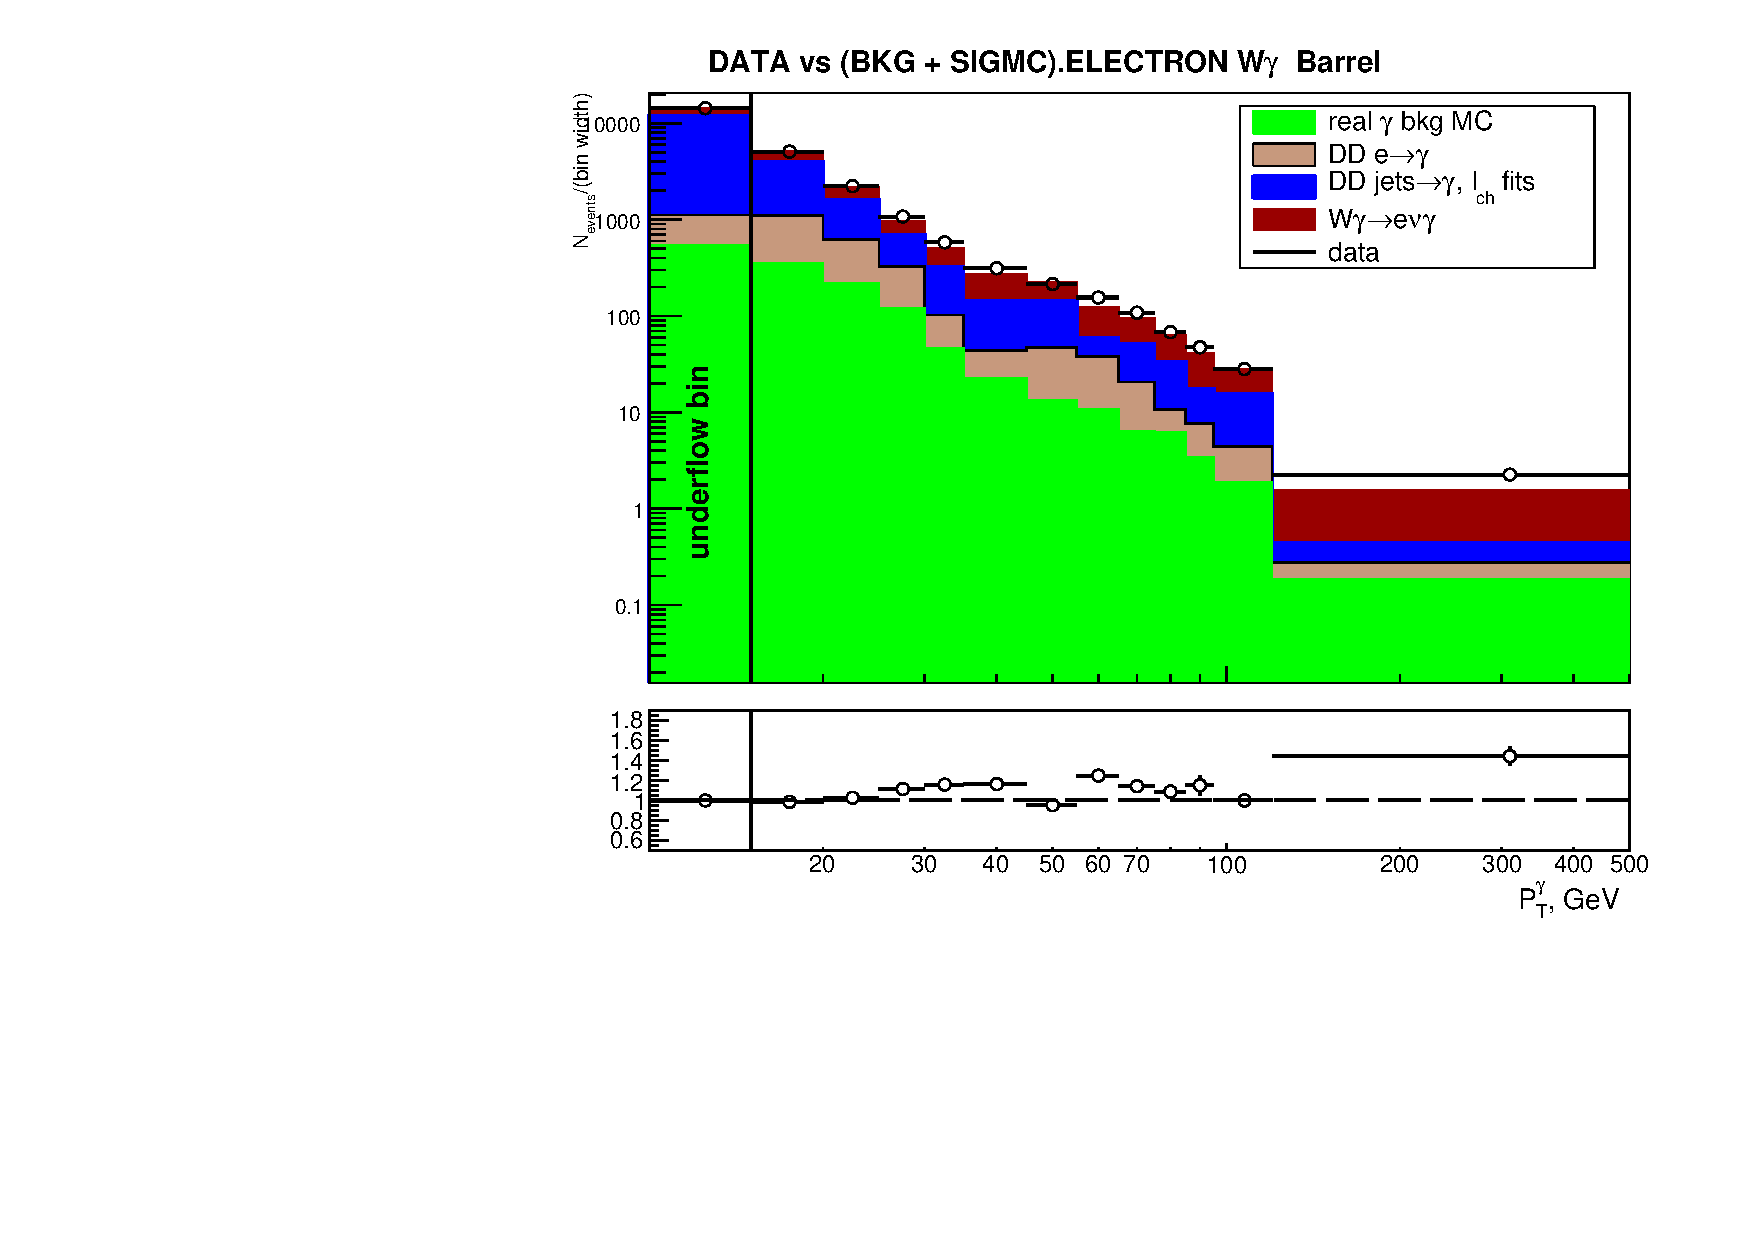
\includegraphics[width=0.40\textwidth]{../figs/figs_v11/ELECTRON_WGamma/PrepareYields/c_DATAvsBkgPlusSigMCc_ELECTRON_WGamma_TEMPL_CHISO_UNblind__Barrel__phoEt.pdf}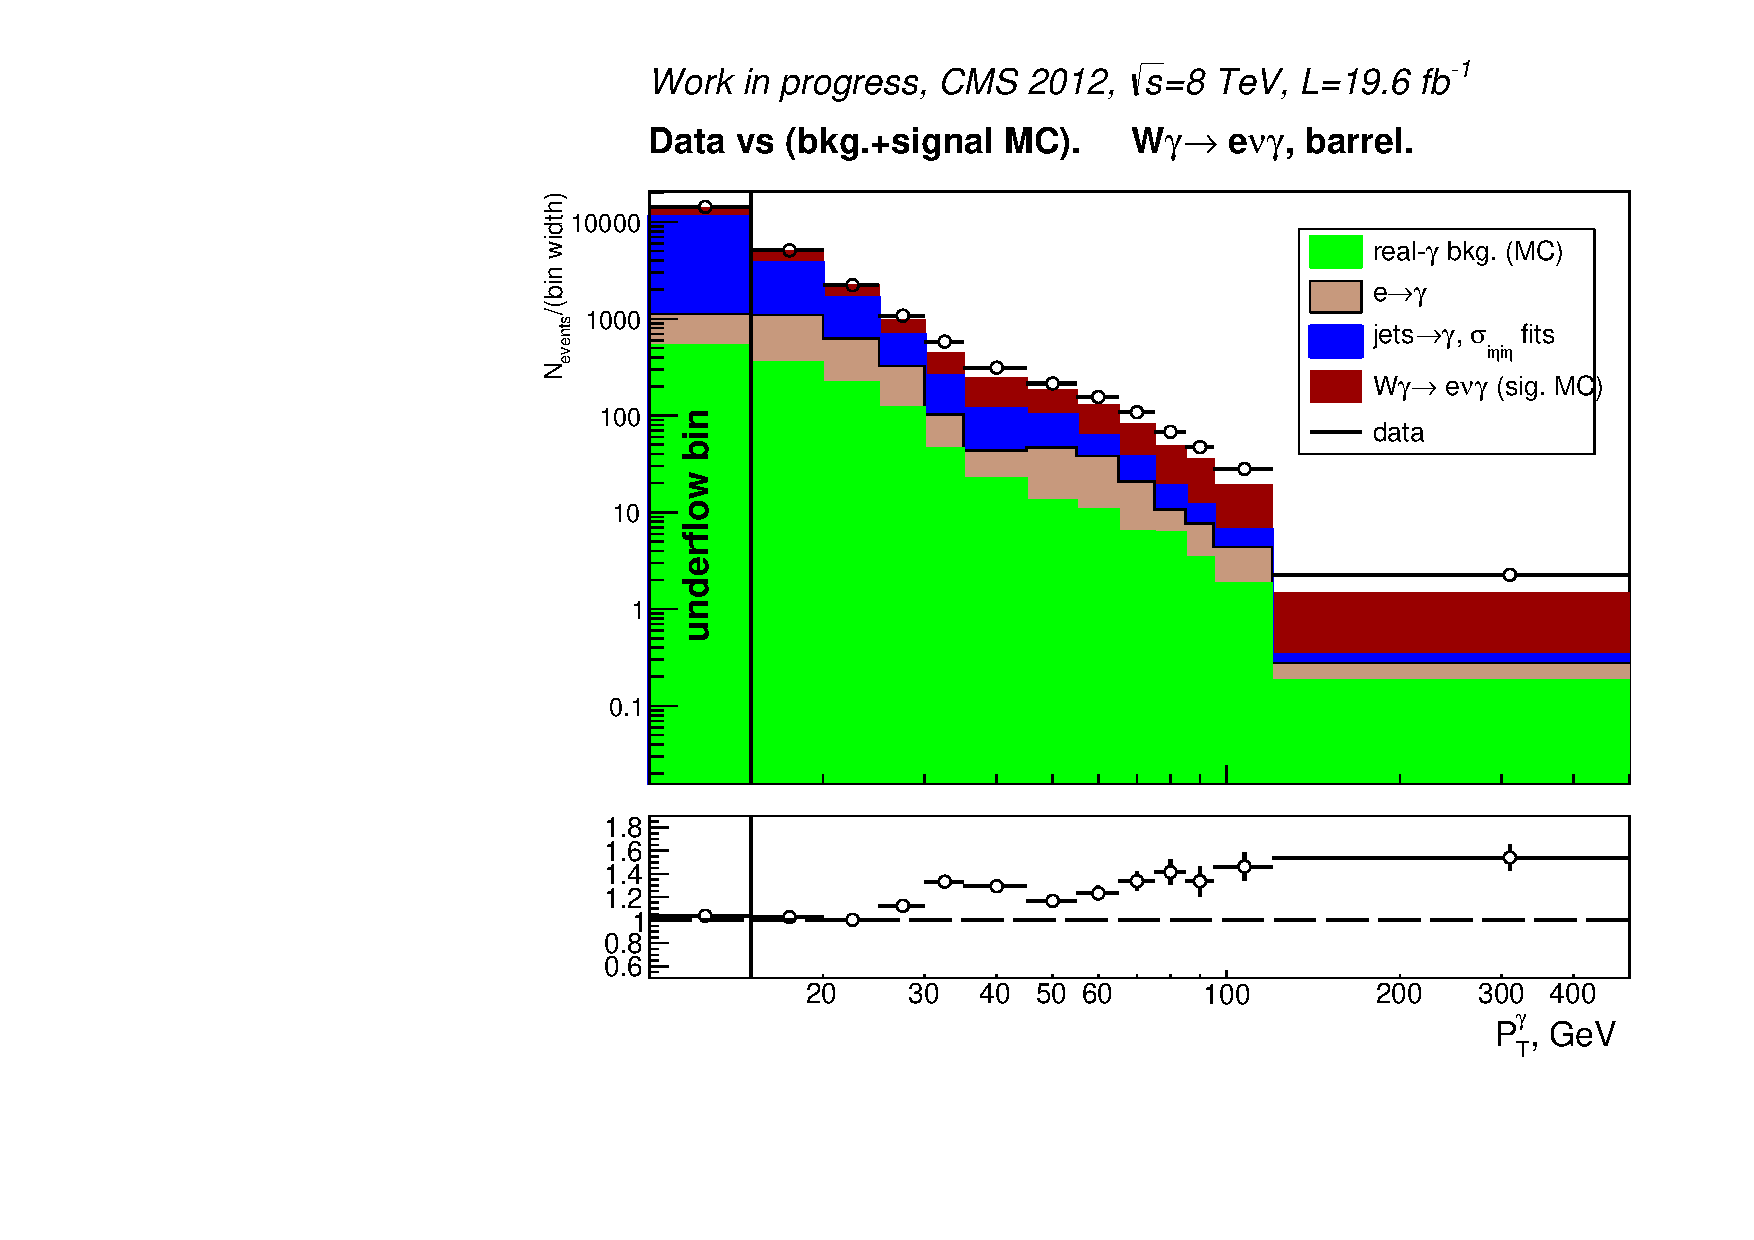
\includegraphics[width=0.40\textwidth]{../figs/figs_v11/ELECTRON_WGamma/PrepareYields/c_DATAvsBkgPlusSigMCc_ELECTRON_WGamma_TEMPL_SIHIH_UNblind__Barrel__phoEt.pdf}\\
    \end{center}
  \end{figure}
\end{frame}%{$jets \rightarrow \gamma$ Background Subtraction. Plots, W$\gamma$}

\begin{frame}\frametitle{\footnotesize{$P_T^{\gamma}$ Spectrum after Background Subtraction (EB and EE)}}
  
  \begin{figure}[htb]
    \begin{center}    
       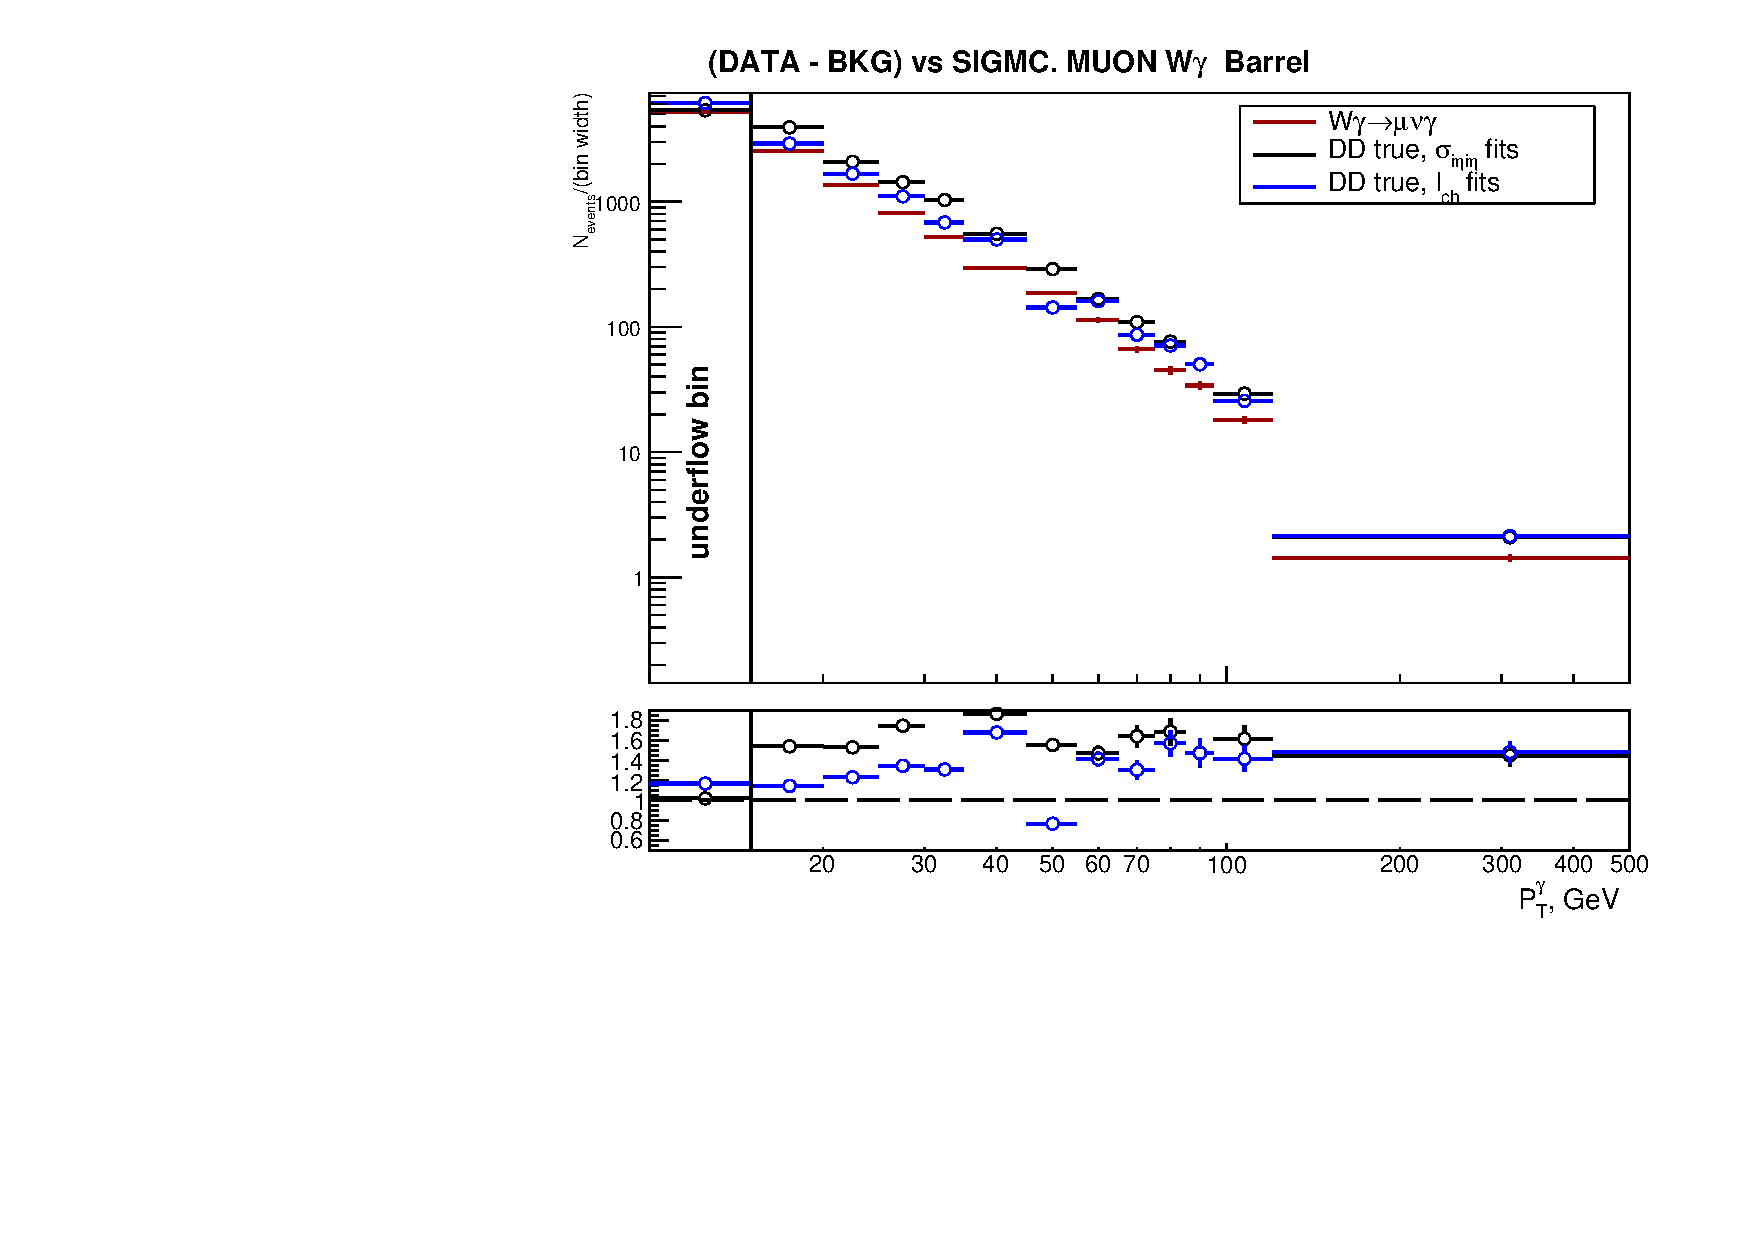
\includegraphics[width=0.40\textwidth]{../figs/figs_v11/MUON_WGamma/PrepareYields/c_BkgSubtrDATAvsSIGMC_c_MUON_WGamma__UNblind__Barrel__phoEt.pdf}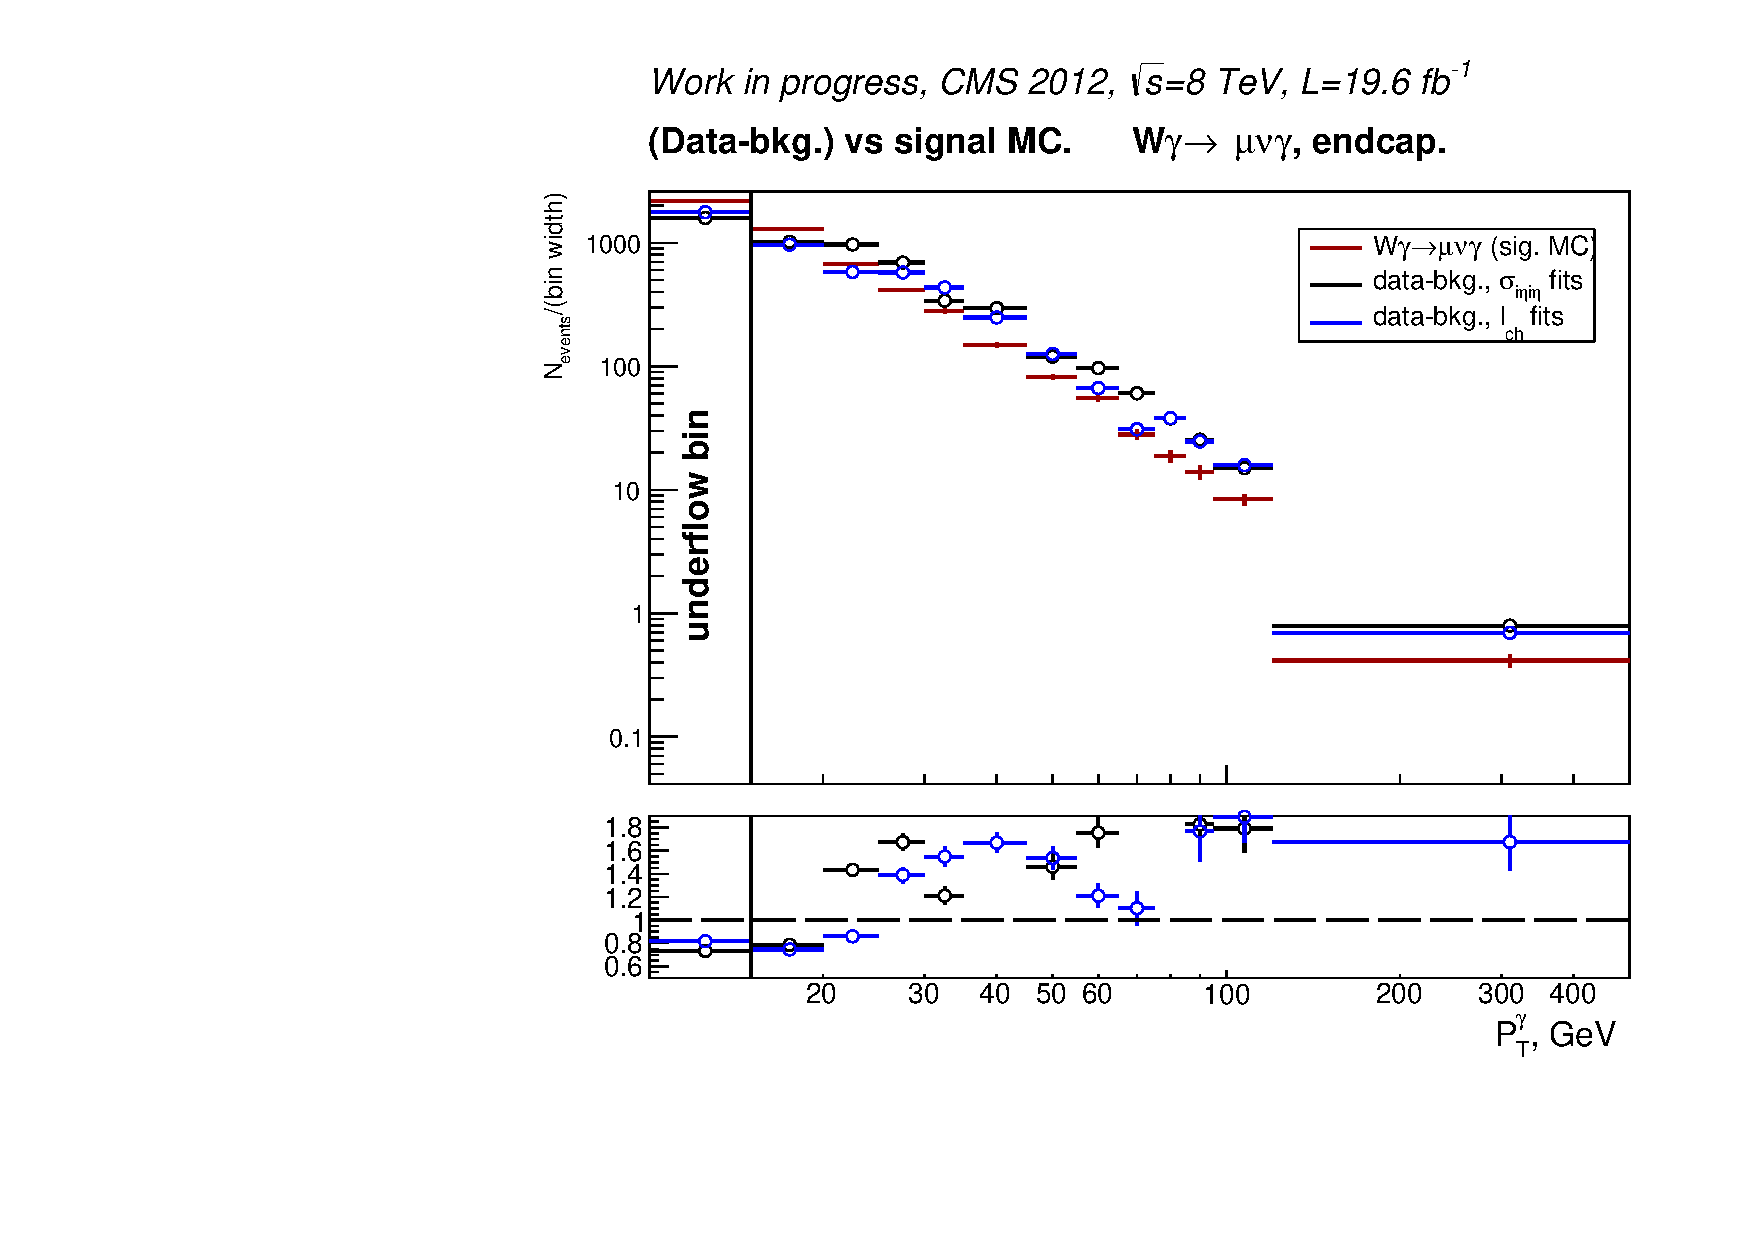
\includegraphics[width=0.40\textwidth]{../figs/figs_v11/MUON_WGamma/PrepareYields/c_BkgSubtrDATAvsSIGMC_c_MUON_WGamma__UNblind__Endcap__phoEt.pdf}\\
       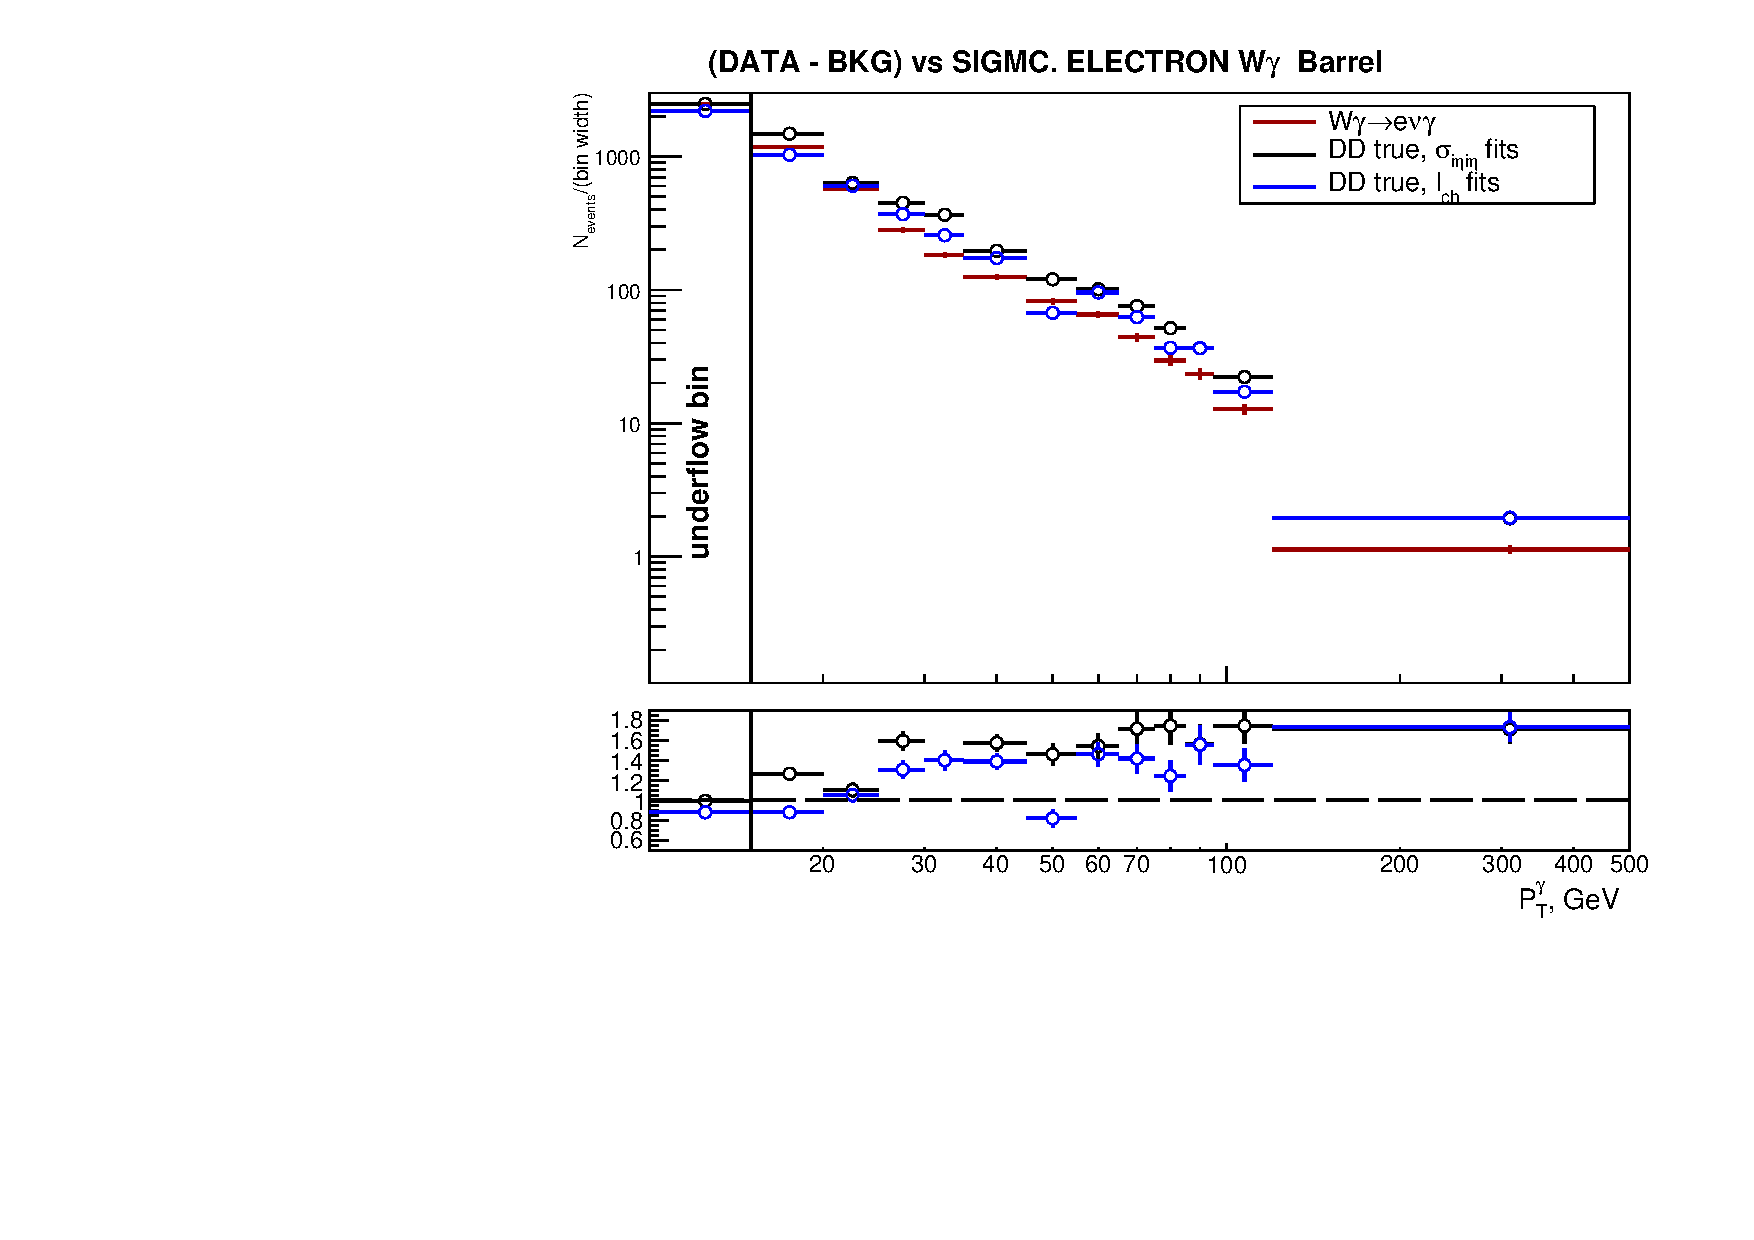
\includegraphics[width=0.40\textwidth]{../figs/figs_v11/ELECTRON_WGamma/PrepareYields/c_BkgSubtrDATAvsSIGMC_c_ELECTRON_WGamma__UNblind__Barrel__phoEt.pdf}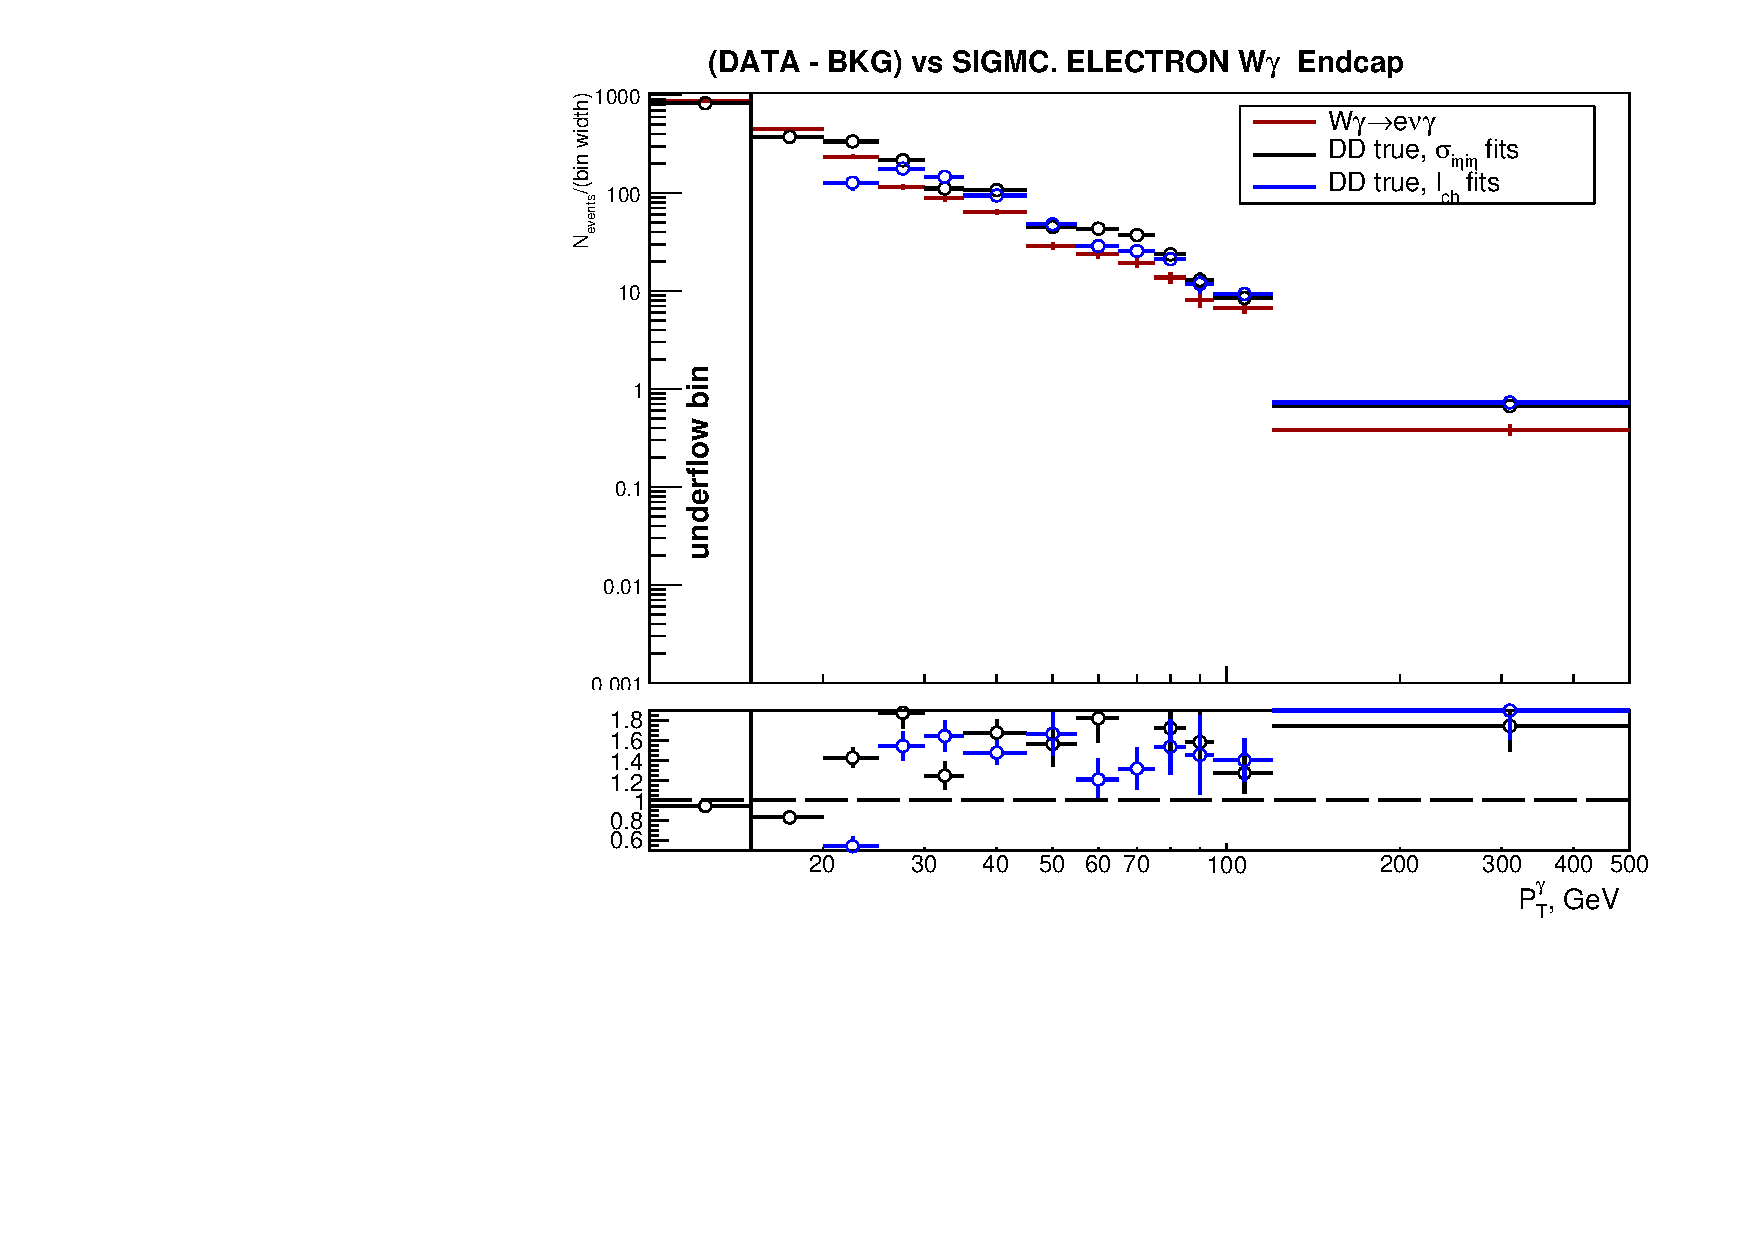
\includegraphics[width=0.40\textwidth]{../figs/figs_v11/ELECTRON_WGamma/PrepareYields/c_BkgSubtrDATAvsSIGMC_c_ELECTRON_WGamma__UNblind__Endcap__phoEt.pdf}\\
    \end{center}
  \end{figure}
\end{frame}%{$jets \rightarrow \gamma$ Background Subtraction. Plots, W$\gamma$}

\begin{frame}\frametitle {Cross Checks for Jets$\rightarrow\gamma$ Background Estimation}

\footnotesize{\bfseries{Simple MC closure check:}}
\tiny
\begin{itemize}
  \item Mix $W\gamma$ and $W$+jets MC samples to prepare pseudodata;
  \item Use $W\gamma$ and $W$+jets Mc to prepare templates;
  \item Fit pseudodata and compare fit results with MC predictions;
  \item Agreement is mostly good.
\end{itemize}

\footnotesize{\bfseries{MC realistic check:}}
\tiny
\begin{itemize}
  \item Mix $W\gamma$, $W$+jets, DY+jets, $Z\gamma$, $t\bar{t}$+jets MC samples to prepare pseudodata-I;
  \item Mix $Z\gamma$ and DY+jets MC to prepare pseudodata-II for templates;
  \item Fit pseudodata-I and compare fit results with MC predictions;
  \item Agreement is better than in data but generally not very good.
\end{itemize}

\footnotesize{\bfseries{$Z\gamma$ check:}}
\tiny
\begin{itemize}
  \item Apply $Z\gamma$ selection on Double Muon and Double Electron datasets;
  \item Prepare templates the same way as for the $W\gamma$ measurement;
  \item Fit $Z\gamma$-selected datasets and compare fit results with MC predictions and $I_{ch}^{\gamma}$ vs $\sigma_{i\etai\eta}^{\gamma}$;
  \item Measure $Z\gamma$ cross section and compare to the published CMS~8~TeV result;
  \item Agreement is very good.
\end{itemize}

\footnotesize{\bfseries{Conclusions: }}\scriptsize{reasons of discrepancies in the $W\gamma$ measurement:  }
\scriptsize
\begin{itemize}
  \item Not accurate shape of templates; 
  \item Effect of a bis on the fit machinery.
\end{itemize}

\end{frame}%{Real-$\gamma$ Backgrounds}
 % real-g, plots for muon and electron channels, cross checks
\begin{frame}\frametitle{Efficiency and Acceptance Correction}

\begin{table}[h]
  \tiny
  \begin{center}
  \begin{tabular}{|l|c|c|}
    \hline
          & \multicolumn{2}{|c|}{{\bfseries{Algebraic representation for}}} \\ 
     {\bfseries{Step}} & \multicolumn{2}{|c|}{{\bfseries{the measurement of}}} \\ 
          & {\bfseries{$d\sigma/dP_{T}^{\gamma}$}} & {\bfseries{$\sigma$}} \\ \hline
    select events & {\bfseries{$N_{sel}^i$}} &    {\bfseries{$N_{sel}$}}       \\ \hline
    subtract background & {\bfseries{$N_{sign}^i = N_{sel}^i - N_{bkg}^i$}} &    {\bfseries{$N_{sign}=N_{sel}-N_{bkg}$}}       \\ \hline
    \multicolumn{3}{|c|}{ } \\  
    \multicolumn{3}{|c|}{NEXT MEASUREMENT STEPS:} \\  
    \multicolumn{3}{|c|}{ } \\ \hline 
    {\bfseries\color{blue}{correct for eff X acc}} & {\color{blue}$N_{ph.sp.}^i = \frac{N_{sign}^i}{(A \times\epsilon)^i}$} &  {\color{blue}$N_{ph.sp.}=\frac{N_{sign}}{A\times\epsilon}$}       \\ \hline
    compute cross section & $ \left( \frac{d\sigma}{dP_{T}^\gamma} \right) ^i = \frac{N_{true}^i}{L \cdot (\Delta P_T^\gamma)^i}$  &  $\sigma = N_{true}/L$       \\ \hline
    \multicolumn{3}{|l|}{estimate systematic uncertainties }         \\ \hline
  \end{tabular}
  \label{tab:analysisOutline}
  \end{center}
\end{table}

\scriptsize
Selection criteria are tighter than the measurement phase space. \\
\tiny
\vspace{3mm}
{\bfseries{Efficiency and acceptance correction:}} {\scriptsize{$N_{ph.sp.}^i = \frac{N_{sign}^i}{(A \times\epsilon)^i}$,}}\\
where $N_{sign}$ is the number of signal ($W\gamma$) events in the selected sample, $N_{ph.sp.}$ is the number of signal events in the measurement phase space.\\
\vspace{3mm}
\scriptsize
\begin{center}
$(A\times\epsilon)^i = \frac{N_{passed(MC)}^i}{N_{passed(MC)}^i+N_{failed(MC)}^i}$, \\
\end{center}
{\tiny where {$N_{passed(MC)}^i$ and $N_{failed(MC)}^i$ are calculated using signal MC simulation sample ($W\gamma$)}}\\

\end{frame}%{Other Corrections}

 % unf-eff-acc, SFs (especially from Wgg)
\begin{frame}\frametitle{Uncertainties}
\scriptsize{\bfseries{Statistical:}} \tiny{limited statistical power of the $W\gamma$-selected dataset}\\
\scriptsize{\bfseries{Systematic:}} \tiny{all other effects including limited stat. of control datasets and MC datasets}\\

  \begin{table}[h]
  \tiny
  \begin{center}
  \begin{tabular}{|l|c|c|}
    \hline
          & \multicolumn{2}{|c|}{Statistical uncertainty propagation} \\ 
     Step & \multicolumn{2}{|c|}{for the measurement of} \\
          & $d\sigma/dP_{T}^{\gamma}$ & $\sigma$ \\ \hline

    select events & $N_{sel}^j \pm \Delta N_{sel}^j$ &    $N_{sel} \pm \Delta N_{sel}$       \\ 
                  & {\color{blue}$\Delta N_{sel}^j = \sqrt{N_{sel}^j}$} &  {\color{blue}$\Delta N_{sel} = \sqrt{N_{sel}}$}   \\ \hline

    subtract background & $N_{sign}^j = N_{sel}^j - N_{bkg}^j$ &    $N_{sign}=N_{sel}-N_{bkg}$       \\ 
                        & {\color{blue}$\Delta N_{sign}^j = \Delta N_{sel}^j$} &    {\color{blue}$\Delta N_{sign} = \Delta N_{sel}$}   \\ \hline

    unfold   & $N_{A\times\epsilon}^i = U_{ij} \cdot N_{sign}^j$ &           \\ 
             & {\color{blue}$\Delta N_{A\times\epsilon}^i$: diagonal elements} &    $-$       \\ 
             & {\color{blue}of the error matrix} &           \\ \hline

    correct for eff X acc & $N_{true}^i = \frac{N_{A\times\epsilon}^i}{(A \times\epsilon)^i}$ &  $N_{true}=\frac{N_{sign}}{A\times\epsilon}$       \\ 
                          & {\color{blue}$\Delta N_{true}^i = \frac{\Delta N_{A\times\epsilon}^i}{(A \times\epsilon)^i}$} &  {\color{blue}$\Delta N_{true}=\frac{\Delta N_{sign}}{A\times\epsilon}$}       \\ \hline

    compute cross section & $ \left( \frac{d\sigma}{dP_{T}^\gamma} \right) ^i = \frac{N_{true}^i}{L \cdot (\Delta P_T^\gamma)^i}$  &  $\sigma = N_{true}/L$       \\ 
                          & {\color{blue}$ \Delta \left[ \left( \frac{d\sigma}{dP_{T}^\gamma} \right) ^i \right]= \frac{\Delta N_{true}^i}{L \cdot (\Delta P_T^\gamma)^i}$ } &  {\color{blue}$\Delta\sigma = \DeltaN_{true}/L$   }    \\ \hline

  \end{tabular}
  \end{center}
\end{table}

\end{frame}%Systematic Uncertainties. Introduction

\begin{frame}\frametitle{Relative Uncertainties [\%]\\ 
          on the $W\gamma\rightarrow\mu\nu\gamma$ Cross Section}
\footnotesize
Diagonal elements of error matrices only
\begin{table}[h]
  \tiny
  \begin{center}
  %\caption{Relative uncertainties [\%]. $W\gamma$, muon channel.}
   \begin{tabular}{|c|c|c|c|c|c|c|c|c|}
    \hline
                   &     & \multicolumn{7}{|c|}{systematic uncertainties}     \\
    $P_T^{\gamma}$,  & stat. & \multicolumn{3}{|c|}{\color{blue}\bfseries{related to jets$\rightarrow\gamma$}} &  &  &  & \\
    GeV           & unc. & {\color{blue}\bfseries{$N_{Ich}$ vs}} &{\color{blue}\bfseries{$Z\gamma$ MC}}      &{\color{blue}\bfseries{templ.}} & SFs & lumi & other & total\\ 
                  &     & {\color{blue}\bfseries{$N_{\sigma{i\eta i\eta}}$}} & {\color{blue}\bfseries{norm.}}    & {\color{blue}\bfseries{stat.}}  &  &  &  & syst.\\ \hline
    $>$15  & 1 & 10 & {\color{blue}\bfseries{24}} & 4 & 2 & 3 & 4 & 27 \\ \hline
 %  10-15 & 2 & 11 & 7 & 8 & 0 & 3 & 6 & 16 \\ \hline
    15-20 & 2 & {\color{blue}\bfseries{31}} & 12 & 10 & 3 & 3 & 6 & 35 \\ \hline
    20-25 & 2 & {\color{blue}\bfseries{29}} & 13 & 11 & 1 & 3 & 6 & 34 \\ \hline
    25-30 & 2 & {\color{blue}\bfseries{24}} & 13 & 11 & 1 & 3 & 5 & 30 \\ \hline
    30-35 & 3 & {\color{blue}\bfseries{40}} & 15 & 13 & 2 & 3 & 7 & 45 \\ \hline
    35-45 & 2 & 11 & {\color{blue}\bfseries{12}} & 8 & 2 & 3 & 6 & 19 \\ \hline
    45-55 & 4 & {\color{blue}\bfseries{62}} & 19 & 20 & 2 & 3 & 8 & 68 \\ \hline
    55-65 & 3 & {\color{blue}\bfseries{15}} & 12 & 14 & 1 & 3 & 7 & 24 \\ \hline
    65-75 & 6 & {\color{blue}\bfseries{36}} & 19 & 17 & 1 & 3 & 10 & 44 \\ \hline
    75-85 & 4 & 6 & 11 & {\color{blue}\bfseries{16}} & 1 & 3 & 10 & 21 \\ \hline
    85-95 & 5 & 2 & 9 & {\color{blue}\bfseries{23}} & 1 & 3 & 13 & 25 \\ \hline
    95-120 & 5 & 10 & 8 & {\color{blue}\bfseries{12}} & 1 & 3 & 9 & 18 \\ \hline
    120-500 & 3 & 4 & 11 & {\color{blue}\bfseries{21}} & 2 & 3 & 9 & 24 \\ \hline
  \end{tabular}
  \label{tab:systInPercent_MUON_WGamma}
  \end{center}
\end{table}
\end{frame}%Systematic Uncertainties. Table. Muon channel

\begin{frame}\frametitle{Relative Uncertainties [\%]\\
  on the $W\gamma\rightarrow e\nu\gamma$ Cross Section}
\footnotesize
Diagonal elements of error matrices only
\begin{table}[h]
  \tiny
  \begin{center}
  %\caption{Relative uncertainties [\%].}
   \begin{tabular}{|c|c|c|c|c|c|c|c|c|c|}
   \hline
                  &       & \multicolumn{8}{|c|}{systematic uncertainties}     \\
    $P_T^{\gamma}$, & stat. & \multicolumn{3}{|c|}{\color{blue}\bfseries{related to jets$\rightarrow\gamma$}} &  &  &  &  & \\
    GeV           & unc.  & {\color{blue}\bfseries{$N_{Ich}$ vs}}          &{\color{blue}\bfseries{$Z\gamma$ MC}} & templ. & {\color{blue}\bfseries{SFs}} & lumi &$e\rightarrow\gamma$ & other & total\\ 
                  &       & {\color{blue}\bfseries{$N_{\sigma{i\eta i\eta}}$}} & {\color{blue}\bfseries{norm.}}       & stat.  &  &  & &  & syst.\\ \hline
    $>$15  & 2 & 15 & {\color{blue}\bfseries{35}} & 5 & 19 & 3 & 4 & 5 & 44 \\ \hline
%    10-15 & 4 & 73 & 20 & 16 & 1 & 3 & 2 & 8 & 78 \\ \hline
    15-20 & 8 & {\color{blue}\bfseries{80}} & 27 & 19 & 17 & 3 & 18 & 11 & 90 \\ \hline
    20-25 & 7 & {\color{blue}\bfseries{38}} & 20 & 14 & 12 & 3 & 11 & 10 & 48 \\ \hline
    25-30 & 5 & {\color{blue}\bfseries{25}} & 16 & 12 & 14 & 3 & 8 & 8 & 36 \\ \hline
    30-35 & 5 & {\color{blue}\bfseries{35}} & 14 & 12 & 14 & 3 & 3 & 8 & 42 \\ \hline
    35-45 & 3 & 14 & 13 & 8 & {\color{blue}\bfseries{18}} & 3 & 2 & 7 & 28 \\ \hline
    45-55 & 8 & {\color{blue}\bfseries{53}} & 20 & 22 & 36 & 3 & 7 & 11 & 71 \\ \hline
    55-65 & 7 & 17 & 12 & 30 & {\color{blue}\bfseries{44}} & 3 & 5 & 10 & 58 \\ \hline
    65-75 & 7 & 23 & 15 & 32 & {\color{blue}\bfseries{44}} & 3 & 4 & 11 & 61 \\ \hline
    75-85 & 8 & 32 & 17 & 27 & {\color{blue}\bfseries{44}} & 3 & 6 & 13 & 64 \\ \hline
    85-95 & 9 & 9 & 7 & 9 & {\color{blue}\bfseries{40}} & 3 & 8 & 14 & 44 \\ \hline
    95-120 & 7 & 19 & 9 & 14 & {\color{blue}\bfseries{44}} & 3 & 5 & 11 & 51 \\ \hline
    120-500 & 4 & 12 & 6 & 24 & {\color{blue}\bfseries{39}} & 3 & 1 & 9 & 48 \\ \hline
  \end{tabular}
  \label{tab:systInPercent_ELECTRON_WGamma}
  \end{center}
\end{table}
\end{frame}%Systematic Uncertainties. Table. Electron channel

\begin{frame}\frametitle{Major Sources of the Systematic Uncertainties}

\footnotesize{\bfseries{Related to jets$\rightarrow\gamma$ background estimation:}}
  \begin{itemize}
     \scriptsize
     \item {\bfseries{Bias in Template Shape and Fit Machinery:}} 
        \begin{itemize}
          \tiny
          \item Estimate as $|N_{Ich}-N_{\sigma{i\eta i\eta}}|$.
         \end{itemize}
     \item {\bfseries{$Z\gamma$ MC Normalization:}}
        \begin{itemize}
          \tiny
          \item Assign uncertainty on the $Z\gamma$ normalization of $\Delta N=$4.6\% (CMS published $Z\gamma$ measurement);
          \item Prepare fake-$\gamma$ templates with $Z\gamma$ MC normalizations of $N\pm\Delta N$;
          \item Perform fits with such deviated templates;
          \item Assign the spread among the three results as an uncertainty.
        \end{itemize}
     \item {\bfseries{Statistical Power of Templates:}}
       \begin{itemize}
          \tiny
          \item Randomize fake-$\gamma$ templates 100 times with Gaussian distribution;
          \item Perform fits with such deviated templates;
          \item Take the Standard deviation of 100 fit results as an uncertainty;
          \item Same for real-$\gamma$ templates (except randomize 20 times, not 100).
       \end{itemize}
     \item Propagate each of three uncertainties through unfolding and other corrections.
  \end{itemize}

\footnotesize{- - - - - - - - - - - - - - - - - - - -}\\
\footnotesize{\bfseries{Related to PixelSeedVeto SF (electron channel only):}}
  \begin{itemize}
  \begin{itemize}
     \tiny
     \item Change SF by $\pm \Delta[SF]$;
     \item From signal MC, obtain new constants for $A \times \epsilon$ and unfolding corrections;
     \item Compute two new cross section values corresponding to $\pm \Delta[SF]$;
     \item Assign the spread among three cross section values as an uncertainty. 
  \end{itemize}
  \end{itemize}
\end{frame}%Major Sources of the Systematic Uncertainties
 % intro, tables, major sources
\begin{frame}\frametitle{Total and Differential Cross Section}
\begin{table}[h]
  \tiny
  \begin{center}
  %\caption{Relative uncertainties [\%]. $W\gamma$, muon channel.}
   \begin{tabular}{|l|c|}
    \hline
                & $\sigma$ ($P_T^{\gamma}>15$~GeV), fb \\ \hline
    NLO theory  & 9101 \\ \hline
    Data, muon channel & 10949 \pm 91 \pm 1463  \\ \hline
    Data, electron channel & 9146 \pm 185 \pm 2213  \\ \hline
  \end{tabular}
  \end{center}
\end{table}
\begin{figure}[htb]
  \begin{center}
   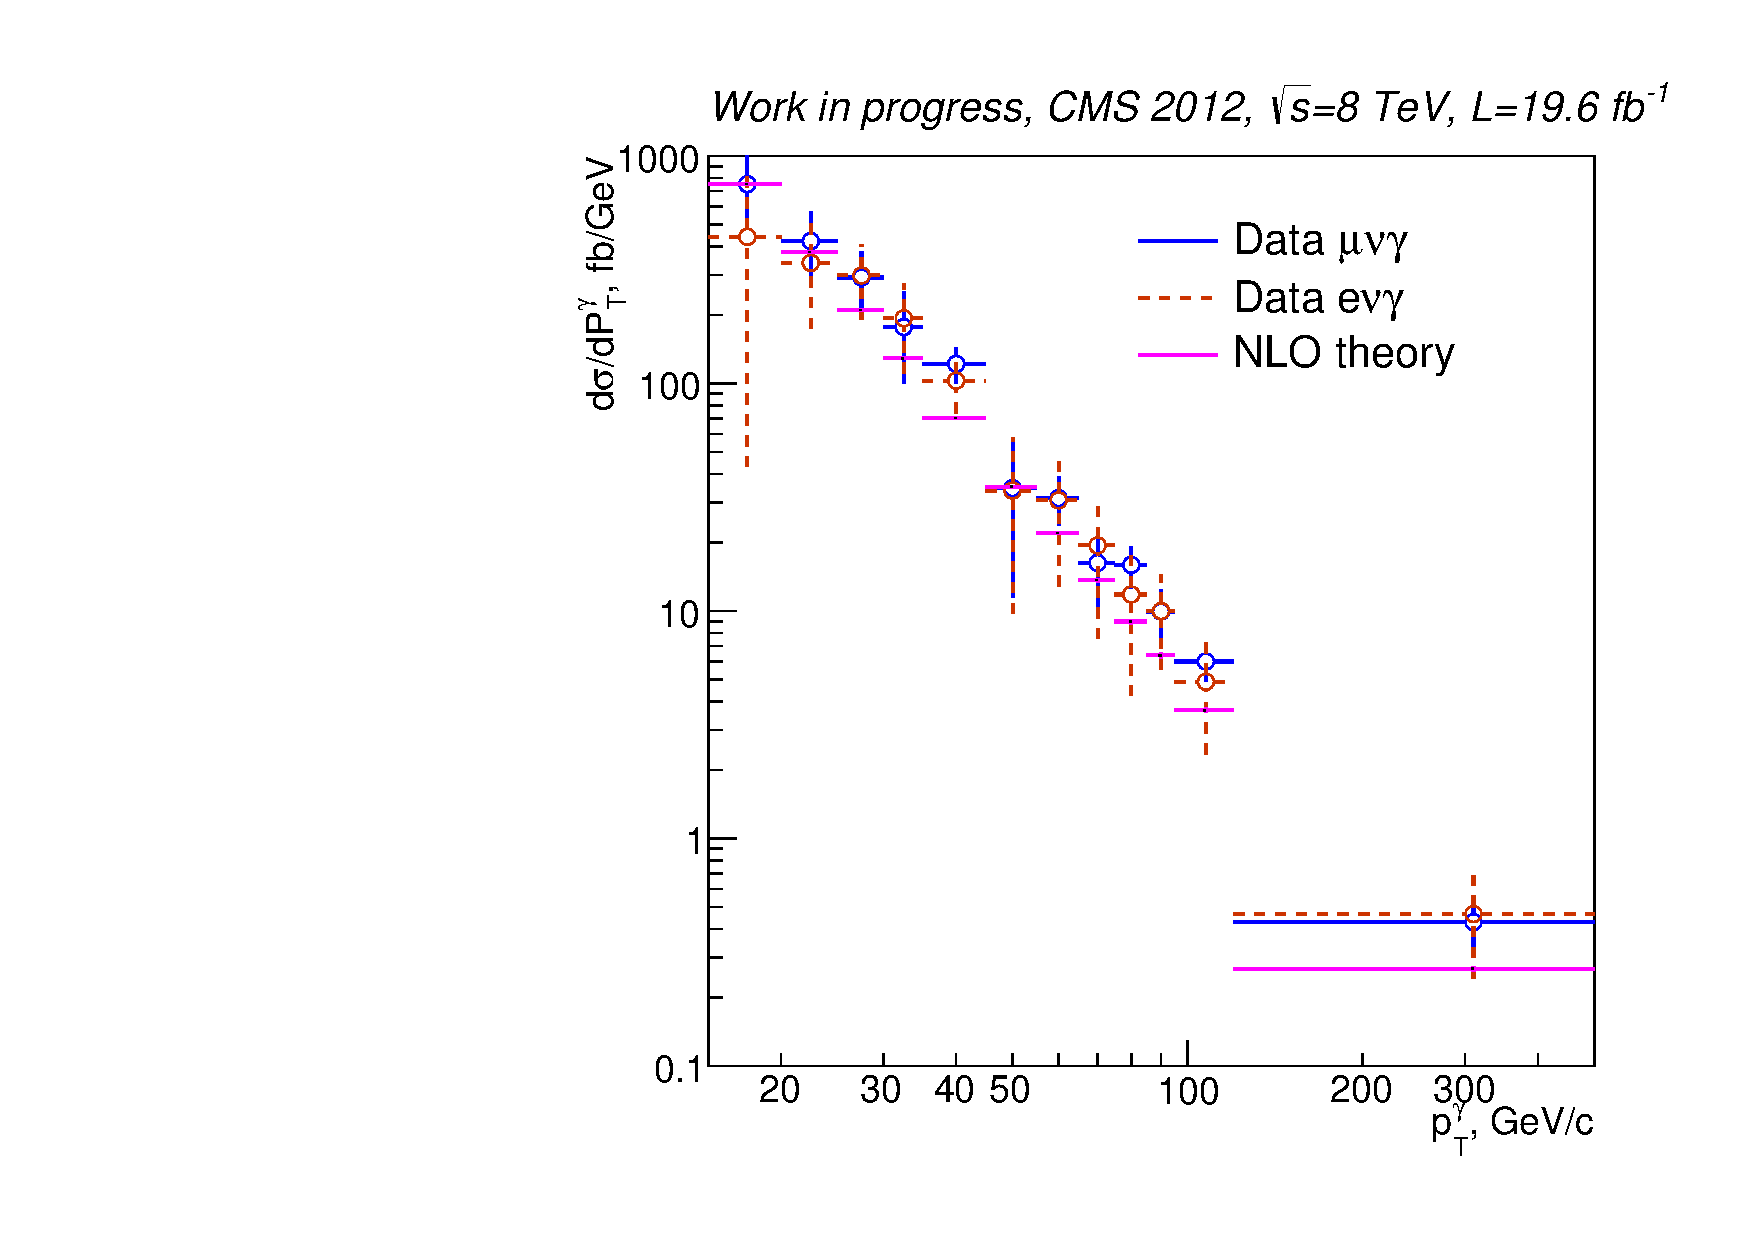
\includegraphics[width=0.49\textwidth]{../figs/figs_v11/ChannelsMERGED_WGamma/CrossSection/compareCSWGamma.pdf}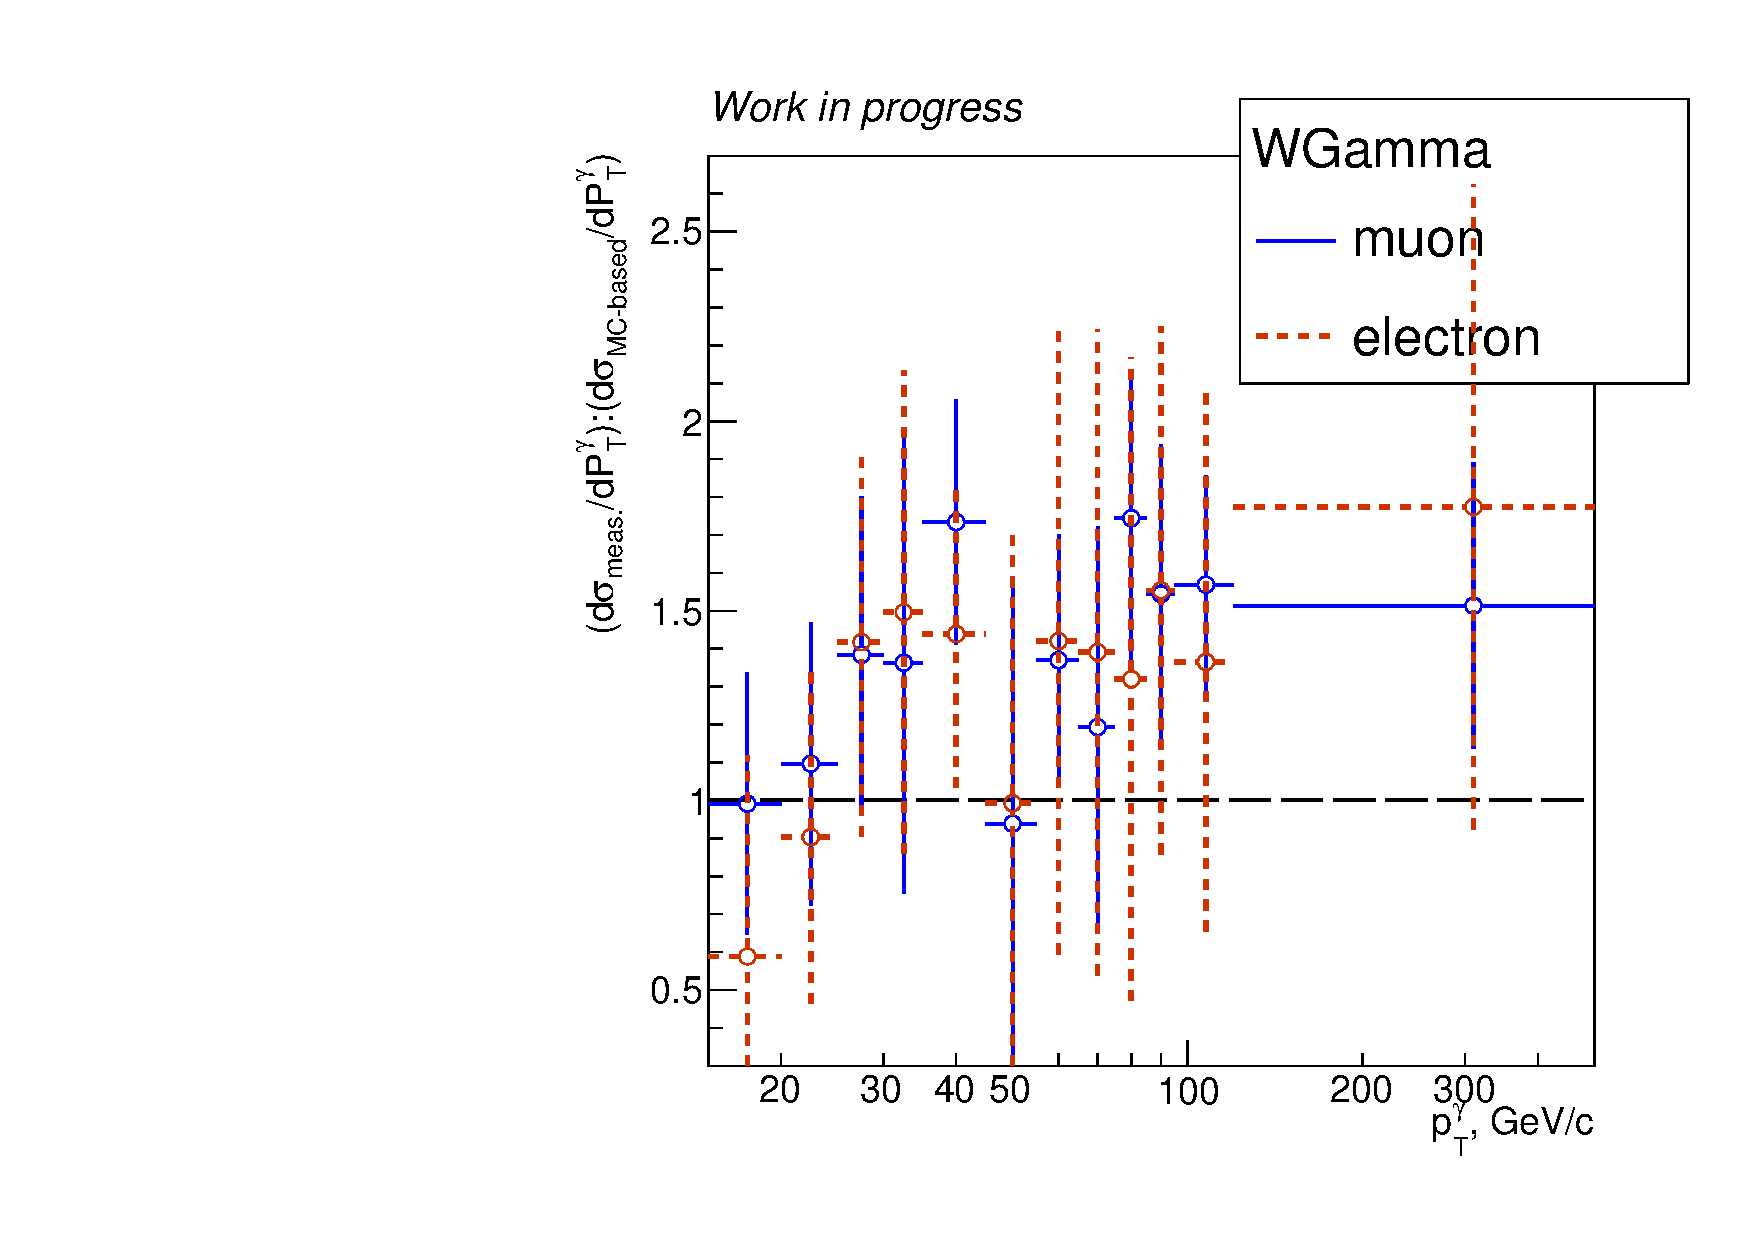
\includegraphics[width=0.49\textwidth]{../figs/figs_v11/ChannelsMERGED_WGamma/CrossSection/compareCSratioTheoryWGamma.pdf}\\
  \end{center}
\end{figure}

\end{frame}%{Differential Cross Section. Plots}

\begin{frame}\frametitle{$Z\gamma$ Check. Differential Cross Section}
\begin{figure}[htb]
  \begin{center}
 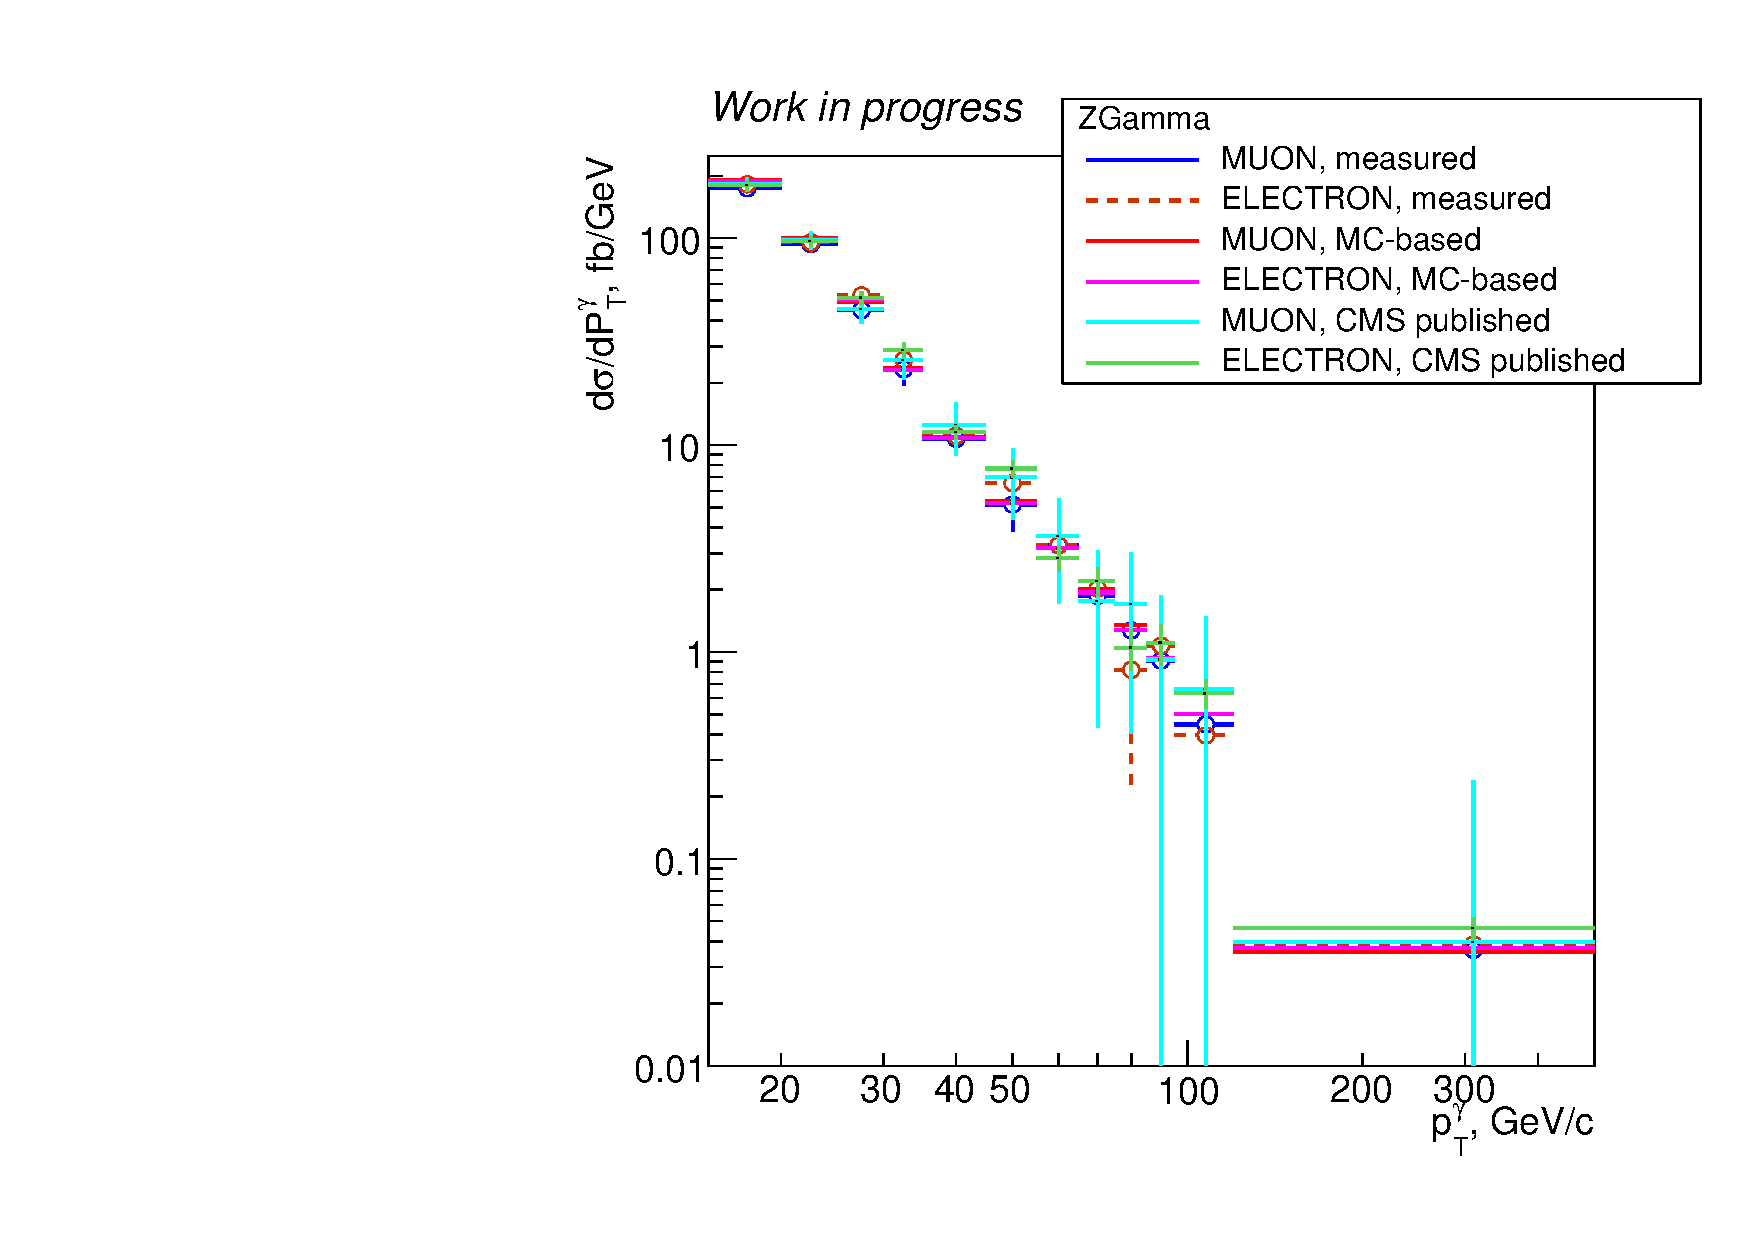
\includegraphics[width=0.49\textwidth]{../figs/figs_v11/ChannelsMERGED_ZGamma/CrossSection/compareCSZGamma.pdf}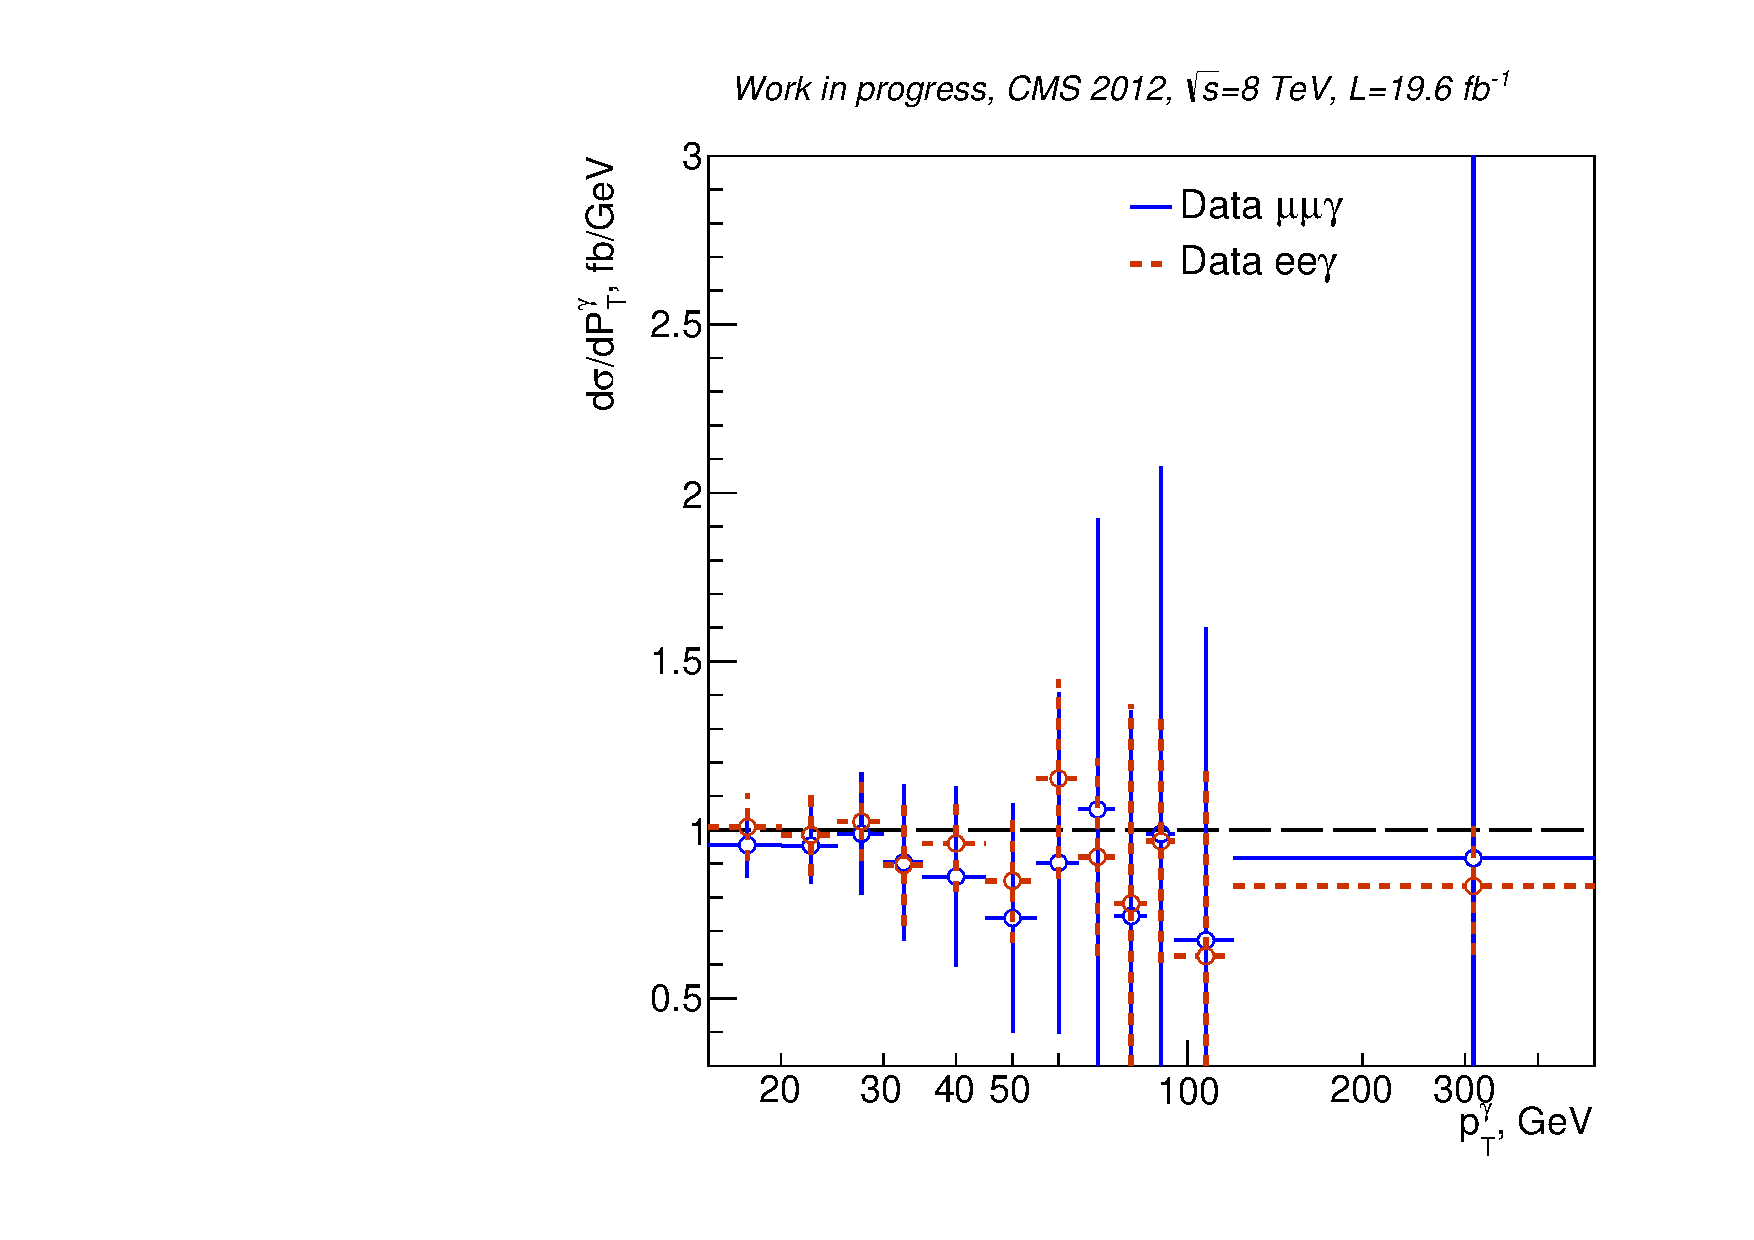
\includegraphics[width=0.49\textwidth]{../figs/figs_v11/ChannelsMERGED_ZGamma/CrossSection/compareCSratioOttoZGamma.pdf}
  \end{center}
\end{figure}
  \tiny
  \begin{itemize}
    \item Cross section of $Z\gamma\rightarrow ll\gamma$ agrees well with the 8 TeV published CMS result and with the theory prediction;
     \item The workflows for the $Z\gamma$ and $W\gamma$ measurements are very similar;
     \item The same procedures of the jets$\rightarrow\gamma$ background estimation have been used;
     \item $Z\gamma\rightarrow\mu\mu\gamma$: template data {\bfseries{significantly overlap}} with analyzed data $\rightarrow$ {\bfseries{closure check}};
     \item $Z\gamma\rightarrow ee\gamma$: template data {\bfseries{do not overlap}} with analyzed data $\rightarrow$ {\bfseries{valid physics measurement}}.
   \end{itemize}
\end{frame}%{$Z\gamma$ Check. Differential Cross Section}
 % Wg cross section, Zg check

\begin{frame}\frametitle{Acknowledgements} % Conclusions
  \scriptsize
  Before drawing conclusions...
  \begin{itemize}
     \item Ilya Kravchenko, Yurii Maravin, Lovedeep Saini;
     \item Joshua Kunkle, Senka Duric, Dmytro Kovalskyi;
     \item Kuo Chia-Ming, Sachiko Toda McBride, Yutaro Iiyama;
     \item whole CMS collaboration.
  \end{itemize}
\end{frame}%{Conclusions}
 

\begin{frame}\frametitle{Conclusions} % Conclusions
  \scriptsize
  \begin{itemize}
     \item Cross section for muon and electron channels are computed; 
     \item This is the first measurement of the differential $W\gamma$ cross section with CMS;
     \item Results agree with the theory;
     \item Results between the two channels agree;
     \item Good agreement in the $Z\gamma$ check validates most parts of the measurement.
  \end{itemize}
\end{frame}%{Conclusions}

\begin{frame}
  \HUGE
  BACKUP
\end{frame}

\begin{frame}\frametitle{Parton Distribution Functions}
  \begin{figure}[htb]
    \begin{center}
       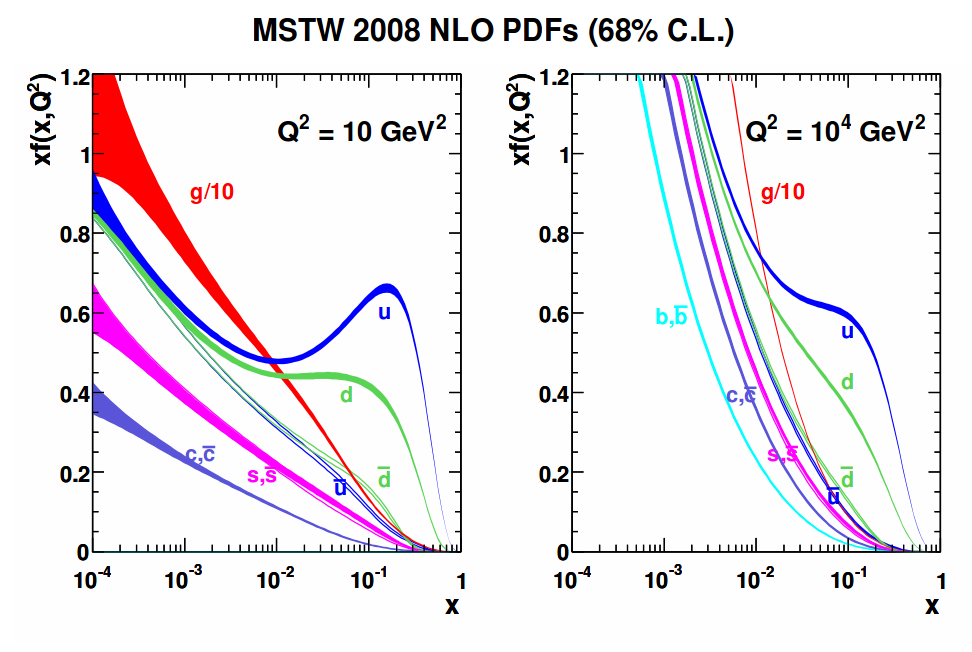
\includegraphics[width=0.80\textwidth]{../figs/Intro/pdfs.png} 
    \end{center}
  \end{figure}
\end{frame}%{WGamma, LO and NLO Feynman diagrams}

\begin{frame}\frametitle{WGamma, LO and NLO Feynman diagrams}
  \begin{figure}[htb]
    \begin{center}
       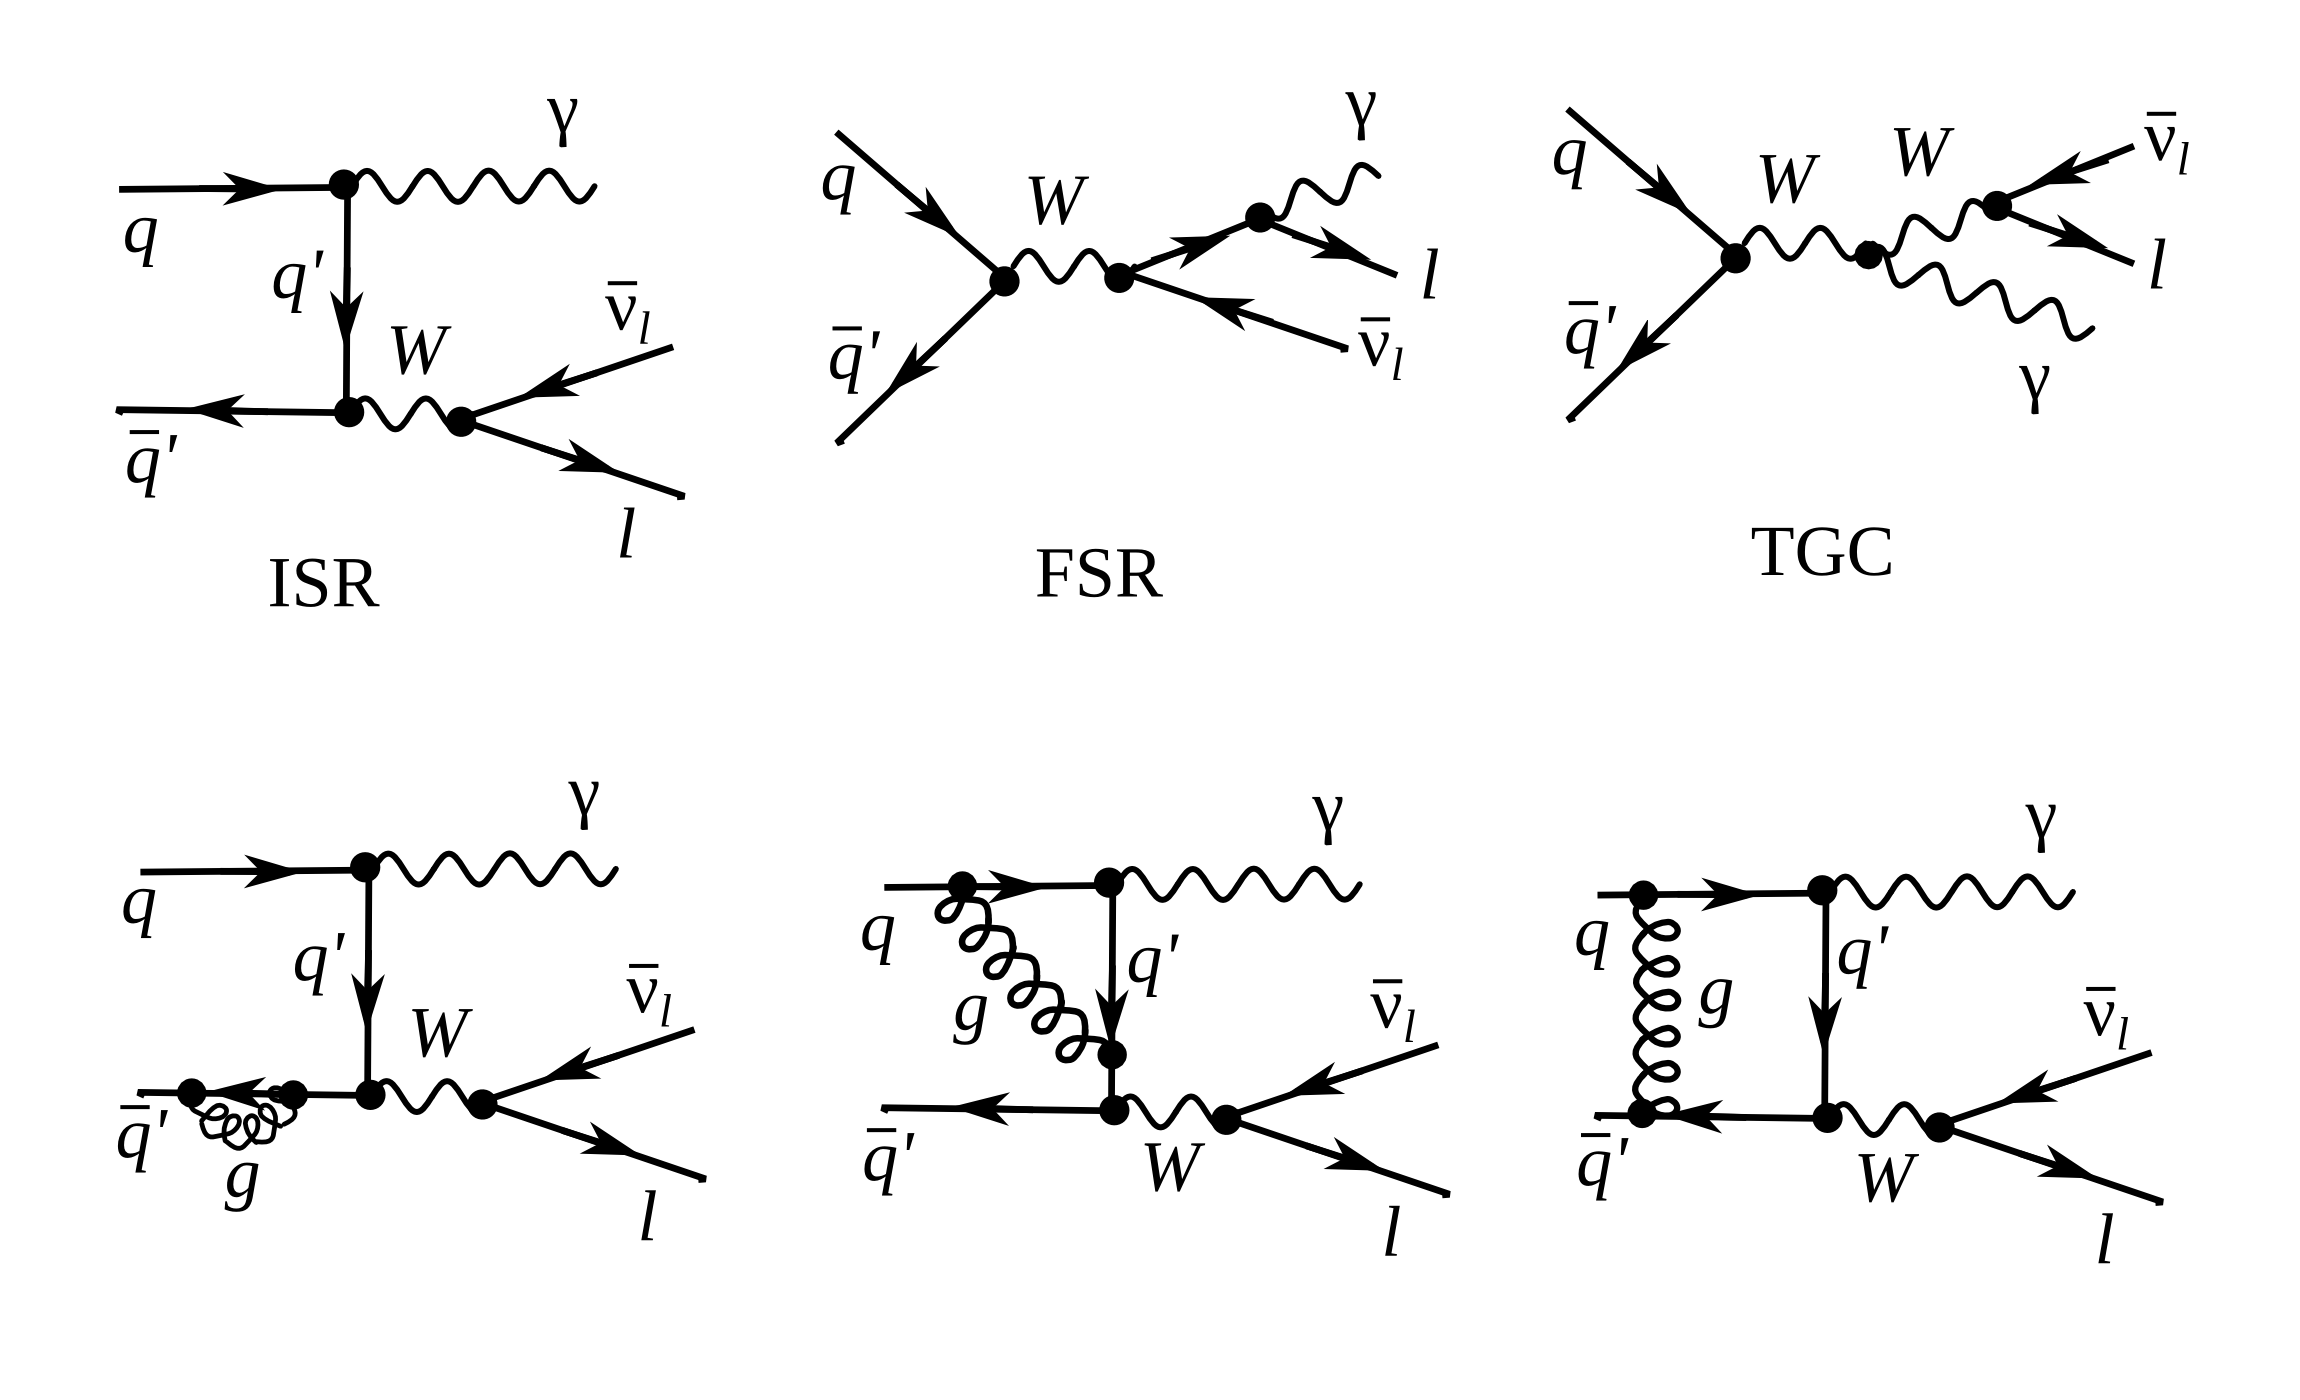
\includegraphics[width=0.85\textwidth]{../figs/WgAbout/feynmWg_LO_NLO.png} 
    \end{center}
  \end{figure}
\end{frame}%{WGamma, LO and NLO Feynman diagrams}

\begin{frame}\frametitle{Data and Simulation Samples}
\scriptsize
Data: CMS experiment, 2012,  $pp$ collisions at $\sqrt{s}=$8~TeV\\
Integrated luminosity: $L=$19.6~fb$^{-1}$ 

\begin{table}[h]
  \scriptsize
  \begin{center}
    \begin{tabular}{|l|l|l|l|}
      \hline
      Dataset          & Candidates                        &  Purpose   & Size, T   \\ \hline
      Single muon      & $W\gamma\rightarrow\mu\nu\gamma$  &  target process   & 1.2 \\ \hline %(NLO MCFM)
      Single electron  & $W\gamma\rightarrow e\nu\gamma$   &  target process   & 2.0 \\ \hline %(NNLO FEWZ)
      Double muon      & $Z\gamma\rightarrow\mu\mu\gamma$  &  background estimation   & 0.4 \\ \hline %(NNLO FEWZ)
      Double electron  & $Z\gamma\rightarrow ee\gamma$     &  background estimation   & 0.5 \\ \hline %(NNLO)
    \end{tabular}
  \end{center}
\end{table} 

\scriptsize
Monte Carlo Simulation (MC) samples:\\

\begin{table}[h]
  \scriptsize
  \begin{center}
 %   \caption{Summary of simulated samples used in the measurement.}
    \begin{tabular}{|l|l|l|}
      \hline
      Process                              & Type & $\sigma$, pb  \\ \hline
      $W\gamma \rightarrow l\nu\gamma$     & signal & 554   \\ \hline %(NLO MCFM)
      $W$+jets$ \rightarrow l\nu $+jets   & background & 36257  \\ \hline %(NNLO FEWZ)
      DY+jets$ \rightarrow ll $+jets     & background & 3504  \\ \hline %(NNLO FEWZ)
      $t\bar{t}$+jets$\rightarrow 1l$+X    & background & 99    \\ \hline %(NNLO)
      $t\bar{t}$+jets$\rightarrow 2l$+X    & background & 24    \\ \hline
      $Z\gamma \rightarrow ll\gamma$       & background & 172   \\ \hline
    \end{tabular}
    \label{tab:mc_bkg_samples}
  \end{center}
\end{table} 

\end{frame}%{MC Samples and Luminosity Reweighting}

\begin{frame}\frametitle{Comment about PU from Wgg CMS Analysis Note}
  \begin{figure}[htb]
    \begin{center}
       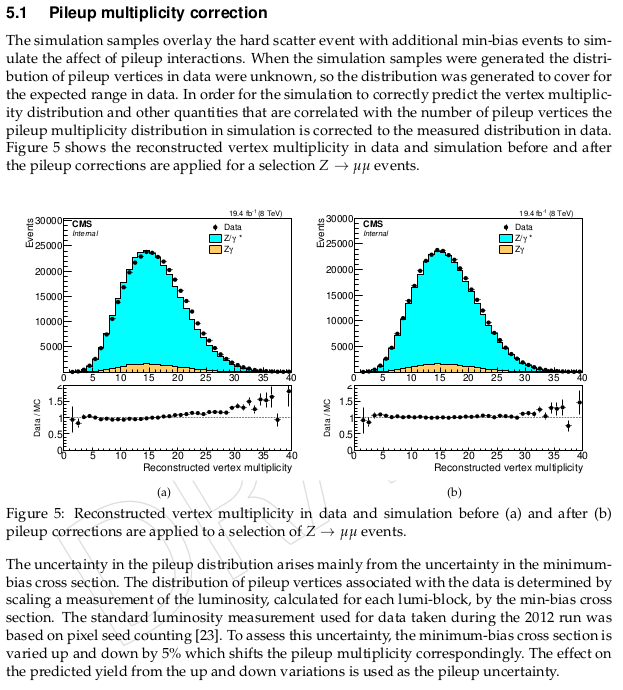
\includegraphics[width=0.65\textwidth]{../figs/ForPresentation/PUmultiplicityCorrection_Wgg.png} 
    \end{center}
  \end{figure}
\end{frame}%{Comment about PU from Wgg note}

\begin{frame}\frametitle{$P_T^{\gamma}$ Spectrum of $W\gamma$ Candidates, Two Channels}
  \begin{figure}[htb]
    \begin{center}
       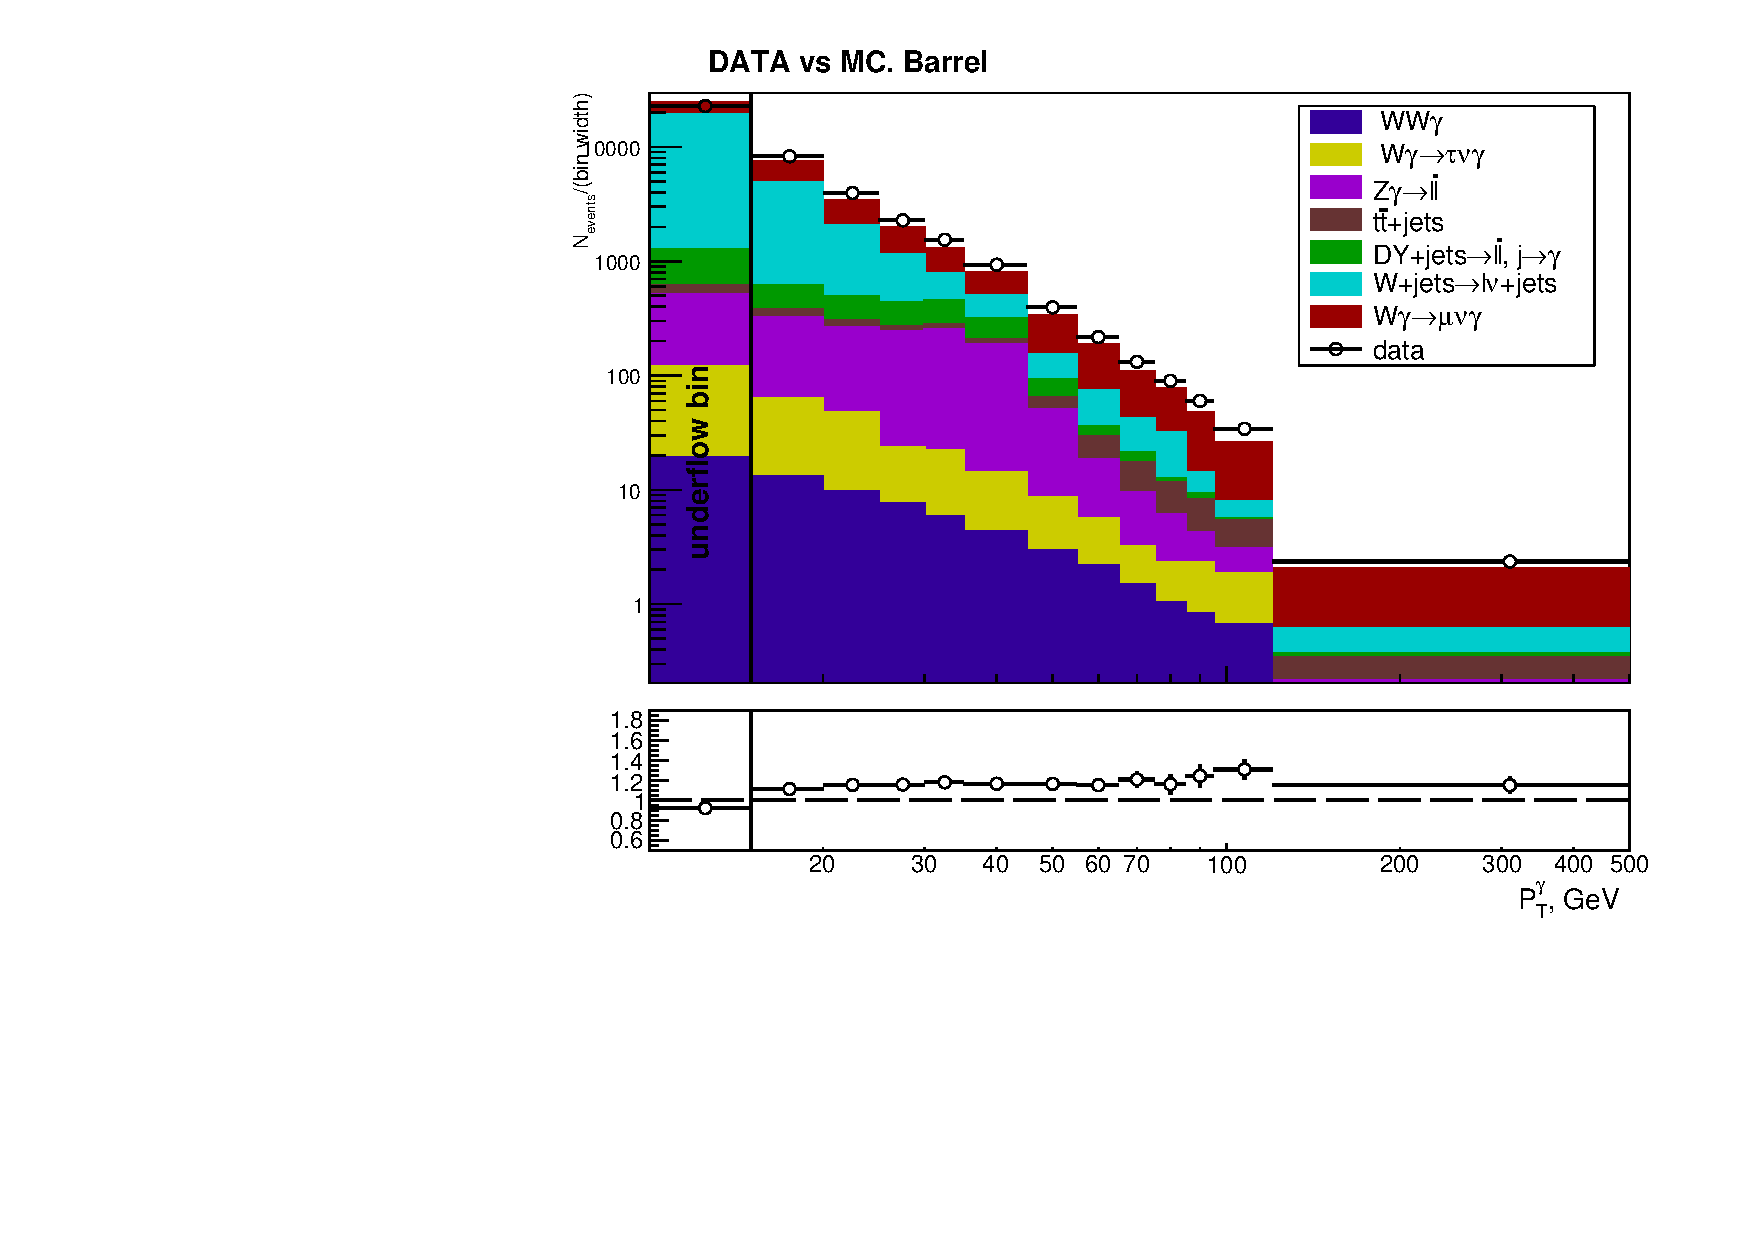
\includegraphics[width=0.49\textwidth]{../figs/figs_v11/MUON_WGamma/PrepareYields/c_TotalDATAvsMC_Barrel__phoEt.pdf} 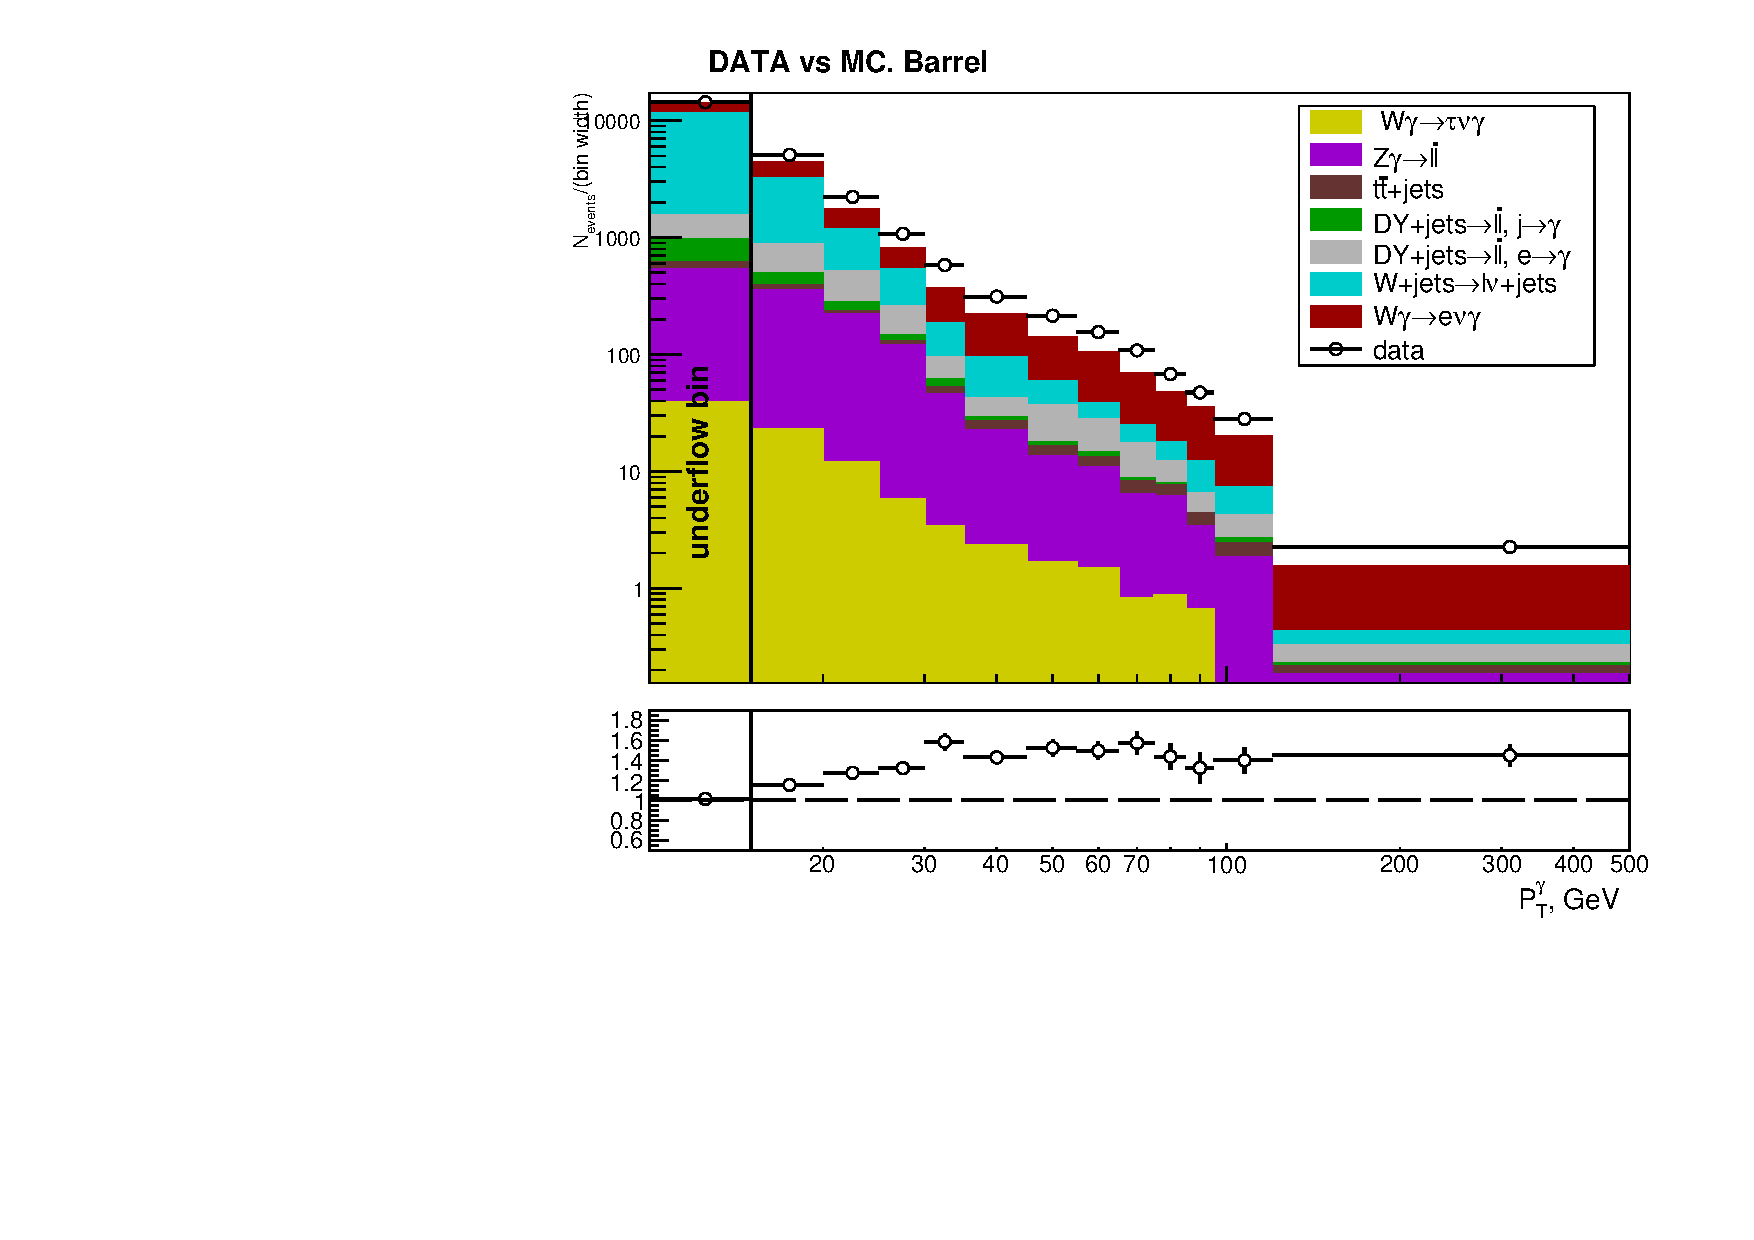
\includegraphics[width=0.49\textwidth]{../figs/figs_v11/ELECTRON_WGamma/PrepareYields/c_TotalDATAvsMC_Barrel__phoEt.pdf} 
    \end{center}
  \end{figure}

\tiny
  \begin{table}[h]
     \tiny
     \begin{center}
     \begin{tabular}{|l|l|}
     \hline
     {\bfseries{Comments:}} &  {\bfseries{ Backgrounds:}}\\ 
     Dominated by $W$+jets events in low $P_T^{\gamma}$ bins; & Jets$\rightarrow\gamma$: $W$+jets, DY+jets, $t\bar{t}$+jets;\\
     Fraction of signal increases with $P_T^{\gamma}$; & $e\rightarrow\gamma$: DY+jets (electron channel only);\\
     Data disagree with MC.          & Real-$\gamma$: $Z\gamma$, $W\gamma\rightarrow\tau\nu\gamma$.\\
     \hline
      \end{tabular}
      \end{center}
  \end{table}

\end{frame}

\begin{frame}\frametitle {$e\rightarrow\gamma$ and Real-$\gamma$ Backgrounds}

  \begin{table}[h]
     \tiny
     \begin{center}
     \begin{tabular}{|l|l|l|l|}
     \hline
     Type & Source & Comment & Estimation \\ \hline
     $e\rightarrow\gamma$ & DY+jets$\rightarrow ee$+jets & no track for $e$; fake $E_T^{miss}$ & semi data driven\\\hline
     Real-$\gamma$ & $Z\gamma \rightarrow ll\gamma$ & pass second lepton veto; fake $E_T^{miss}$ & MC-based\\\hline
     Real-$\gamma$ & $W\gamma \rightarrow \tau\nu\gamma$ & $\tau^- \rightarrow \mu^- \bar{\nu_{\mu}} \nu_{\tau}$ and $\tau^- \rightarrow e^- \bar{\nu_{e}} \nu_{\tau}$ & MC-based\\
     \hline
      \end{tabular}
      \end{center}
  \end{table}

\begin{figure}[htb]
  \begin{center}
   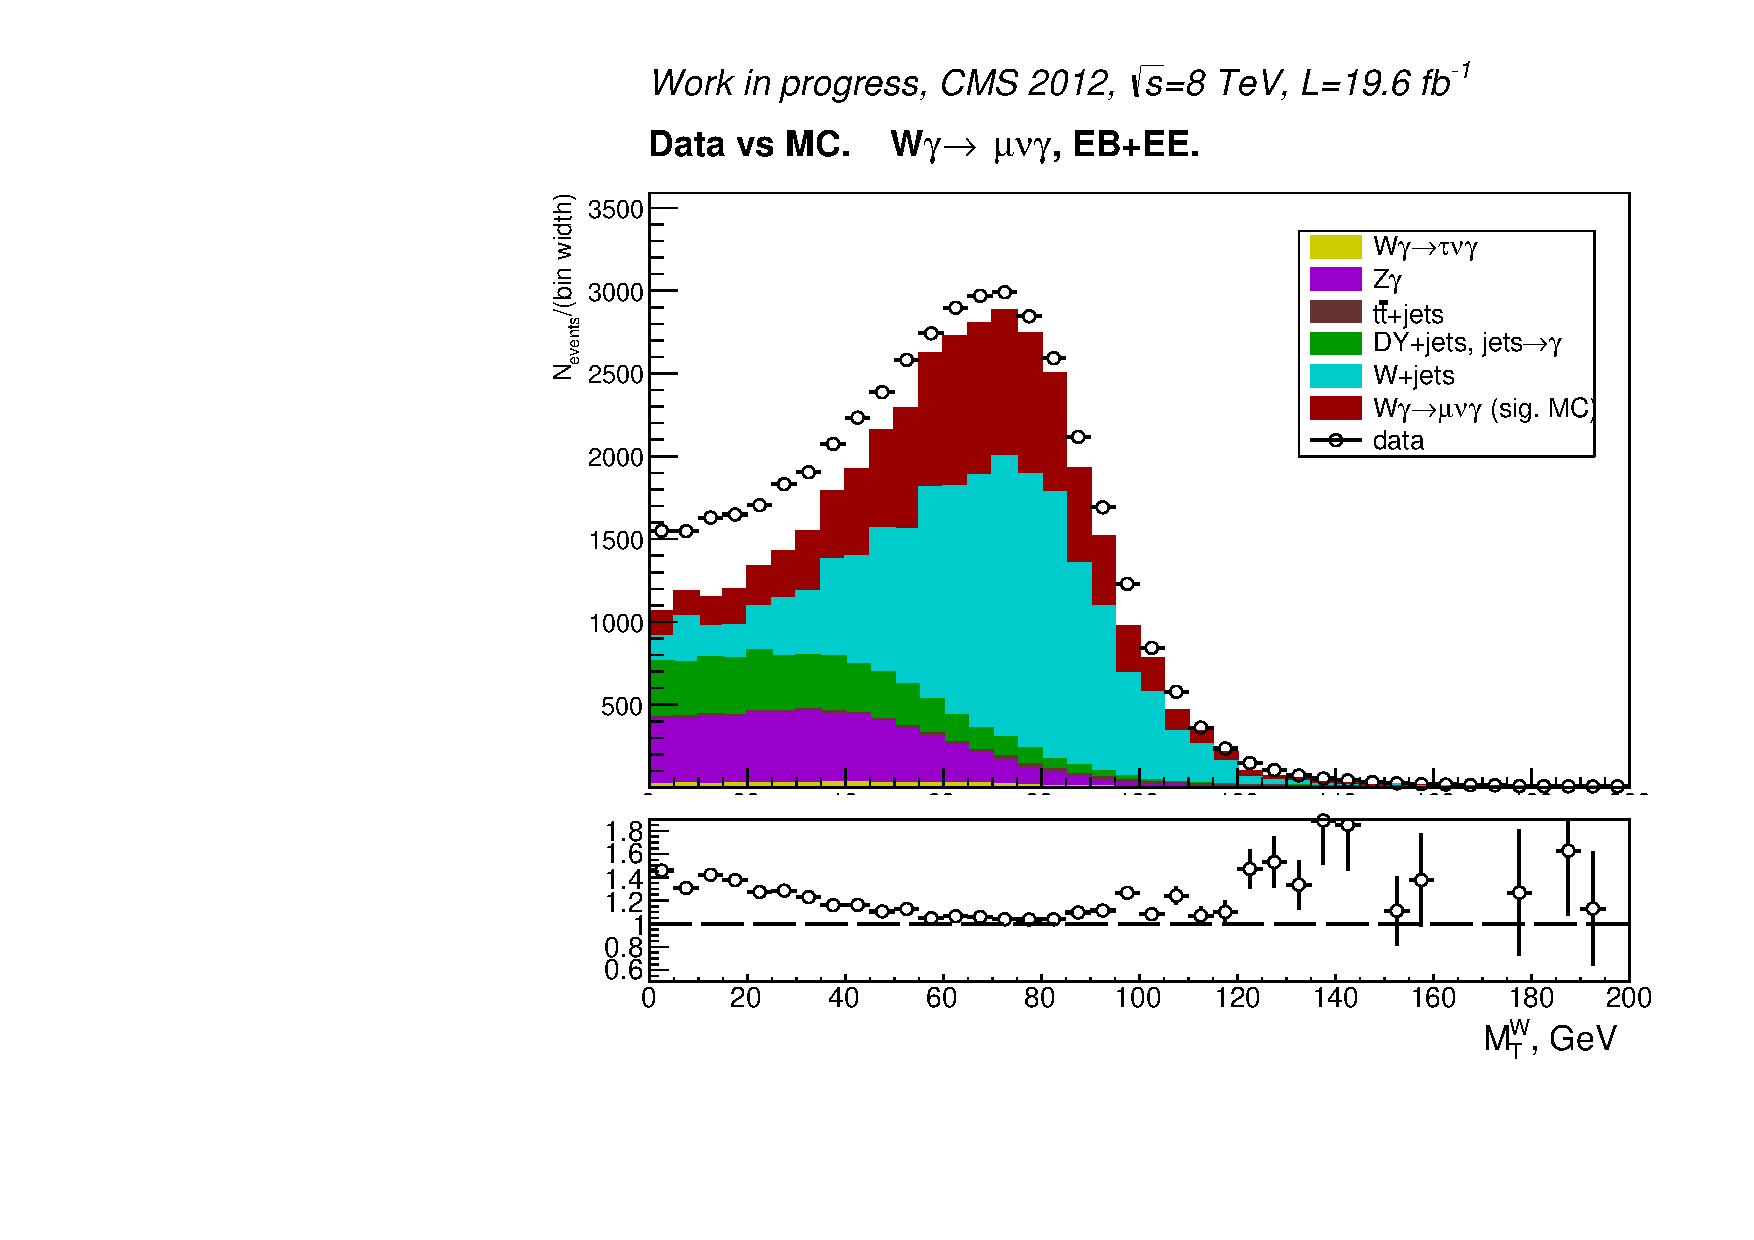
\includegraphics[width=0.32\textwidth]{../figs/figs_v11/MUON_WGamma/PrepareYields/c_TotalDATAvsMC_EtaCommon__WMtVERY_PRELIMINARY.pdf}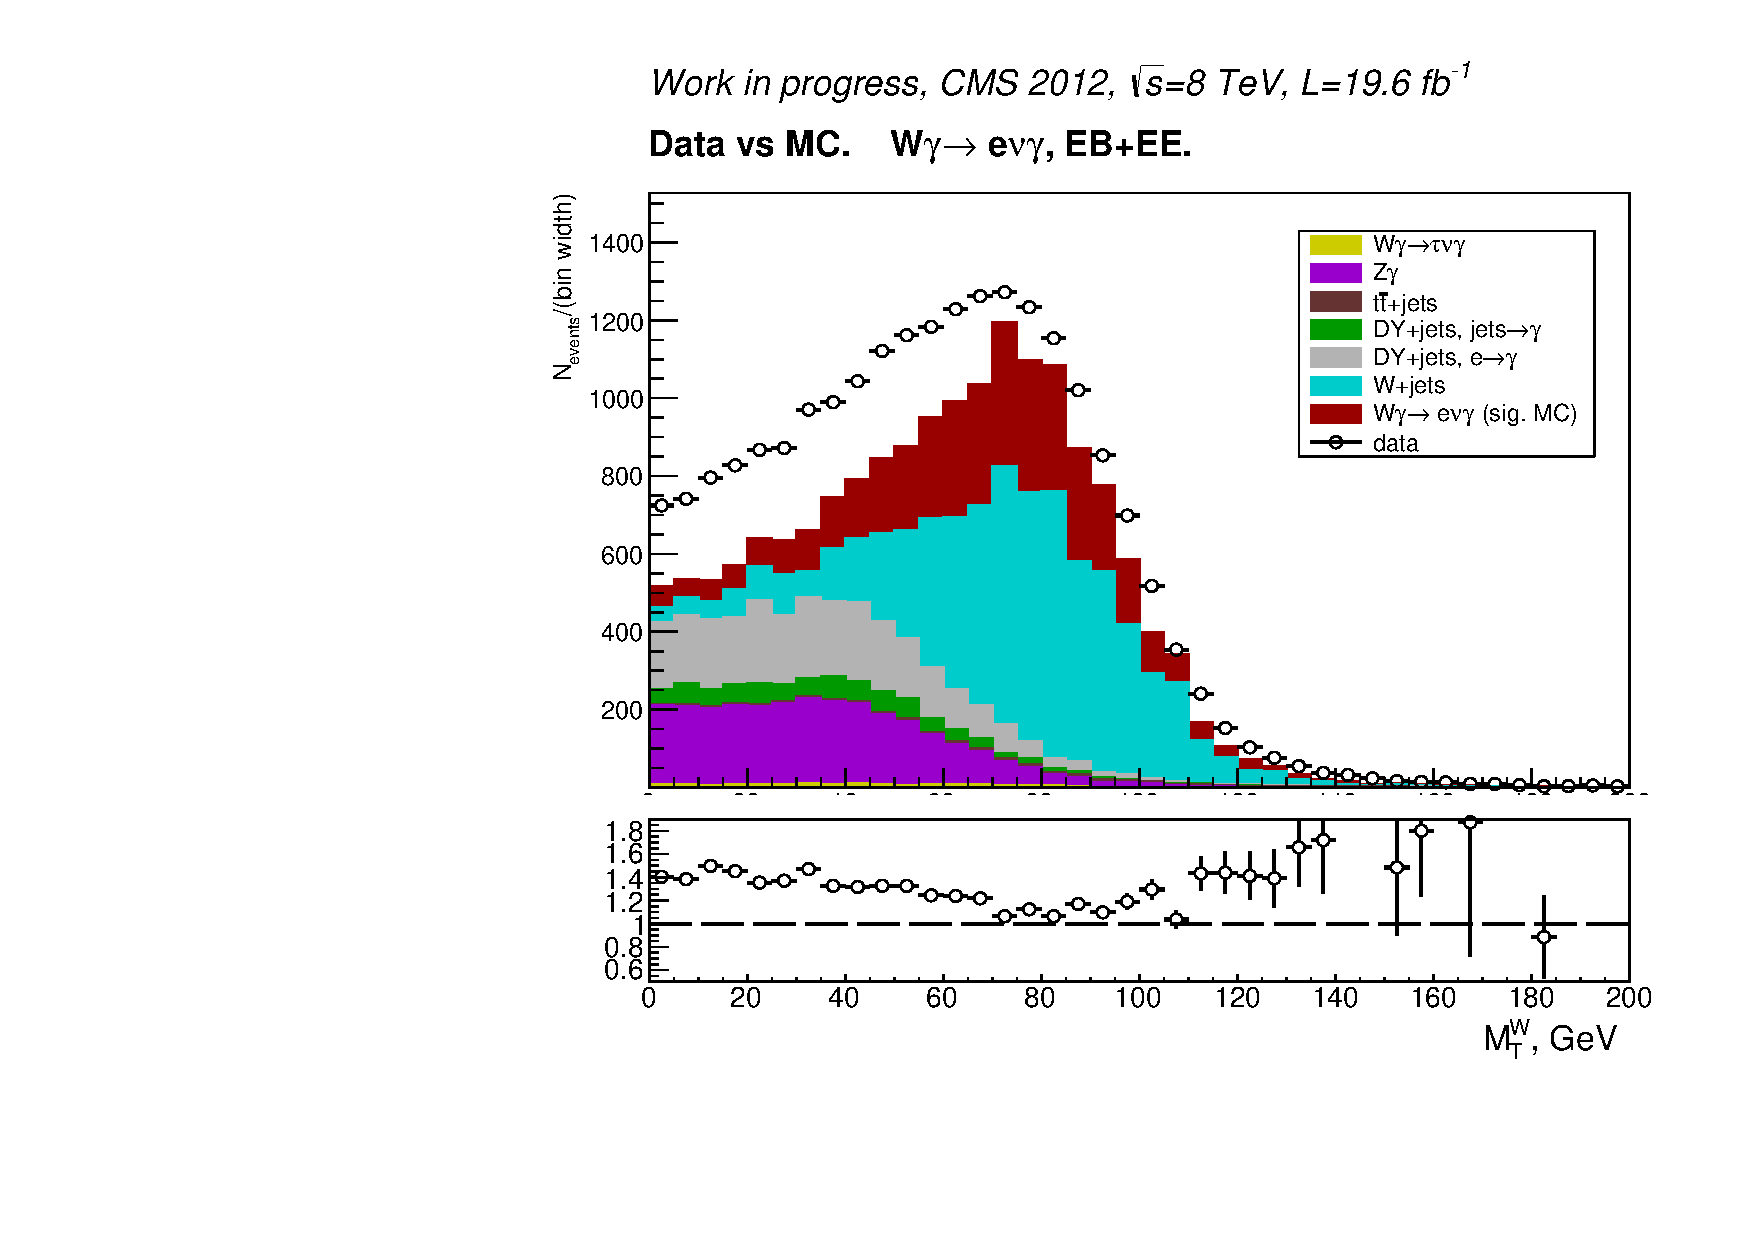
\includegraphics[width=0.32\textwidth]{../figs/figs_v11/ELECTRON_WGamma/PrepareYields/c_TotalDATAvsMC_EtaCommon__WMtVERY_PRELIMINARY.pdf}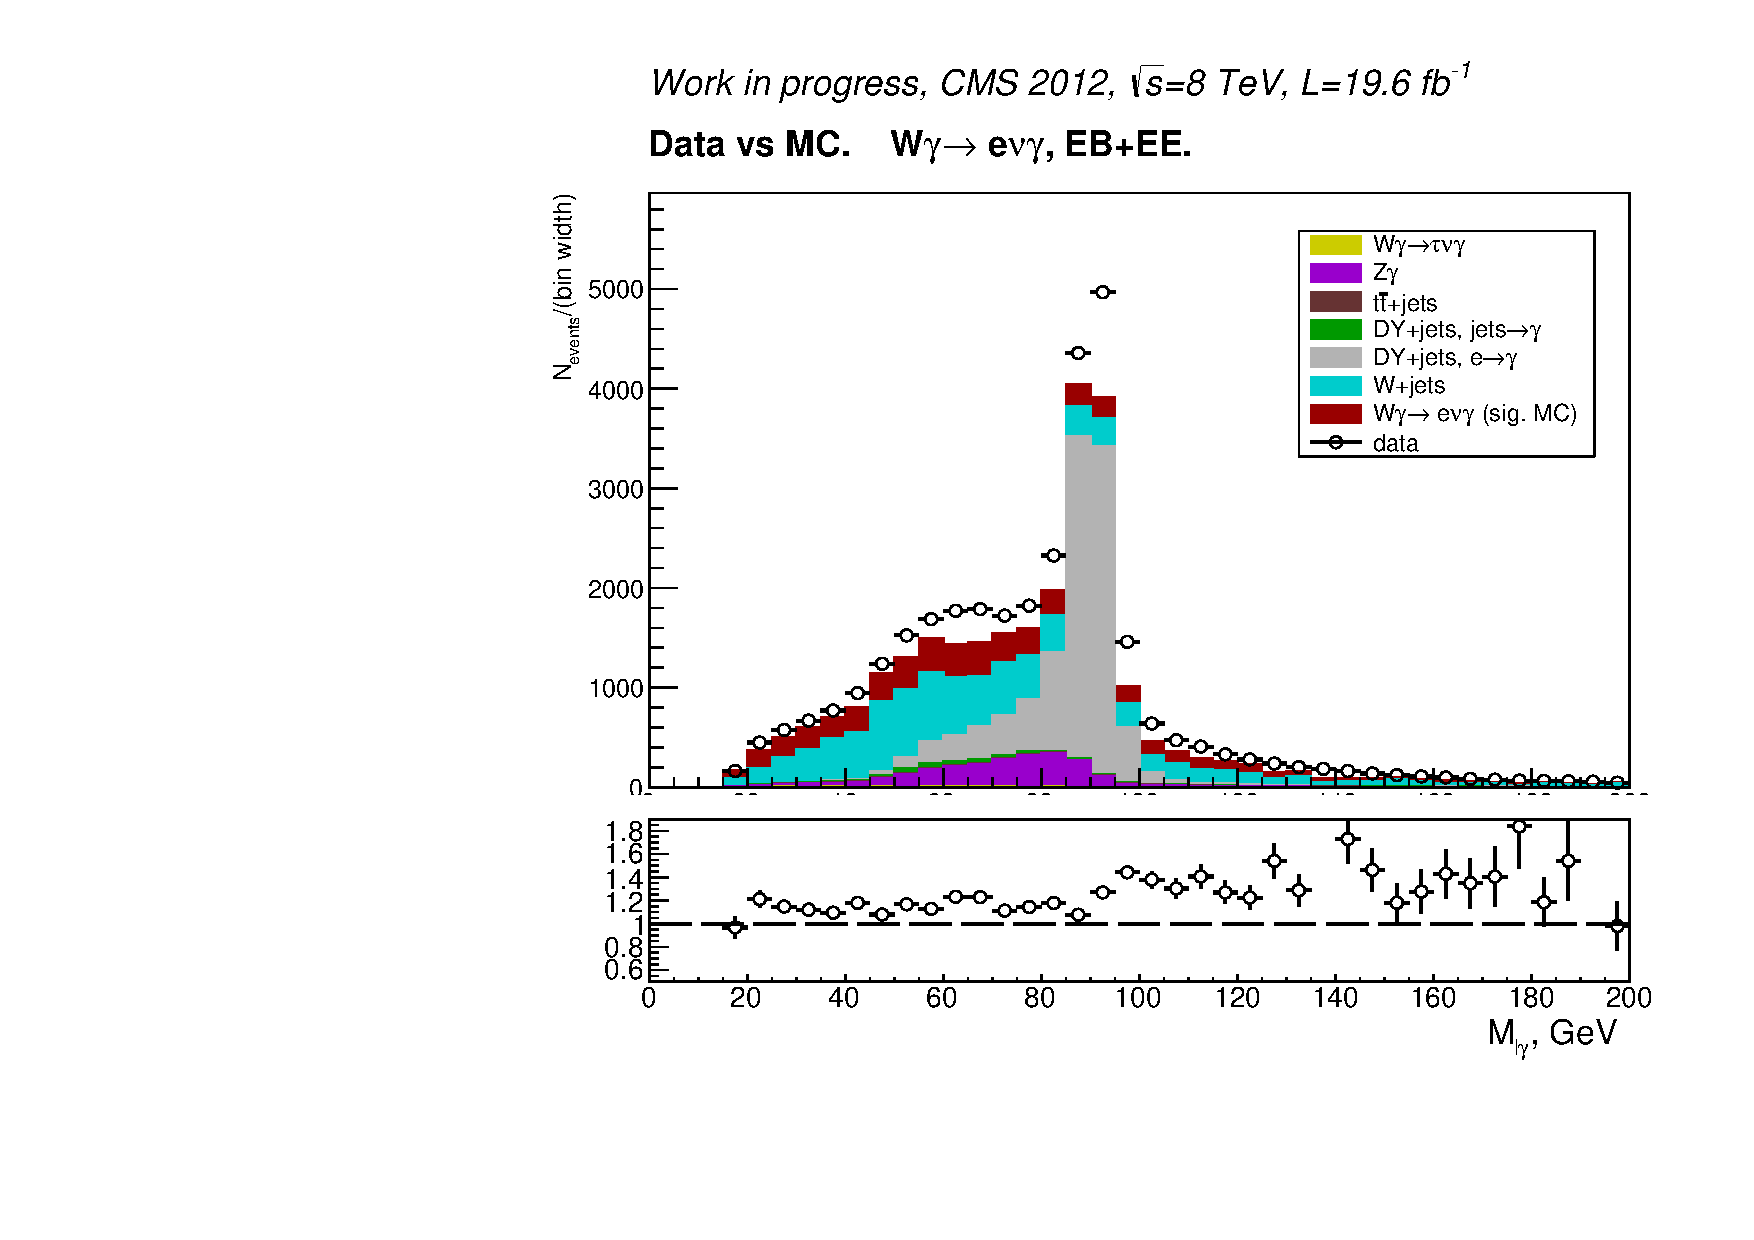
\includegraphics[width=0.32\textwidth]{../figs/figs_v11/ELECTRON_WGamma/PrepareYields/c_TotalDATAvsMC_EtaCommon__Mpholep1PRELIMINARY_FOR_E_TO_GAMMA_WITH_PSV_CUT.pdf}
  \end{center}
\end{figure}
\tiny
$M_T^W>40$~GeV in both channels: rejects events without $E_T^{miss}$\\
$M_{l,\gamma}<70~or~M_{l,\gamma}>110$~GeV in the electron channel: rejects events from DY+jets$\rightarrow ee$+jets \\
{\bfseries{Non-negligible amount remains}}\\
\begin{itemize}
  \item Invariant mass of a particle system ($M_{ab} = m_a^2+m_b^2+2(E_aE_b-{\bfseries{p_a\cdot p_b}})$)
  \item Transverse mass of a $W$ boson ($M_T^W=\sqrt{2  P_T^{l}  E_T^{miss}  (1-\cos{(\phi^{l}-\phi^{miss})})}$)
\end{itemize}

\end{frame}%{$e\rightarrow\gamma$ and Real-$\gamma$ Backgrounds}

\begin{frame}\frametitle{\footnotesize{$P_T^{\gamma}$ Spectrum (ECal Barrel Only). Both channels}}
   \begin{figure}[htb]
    \begin{center}
       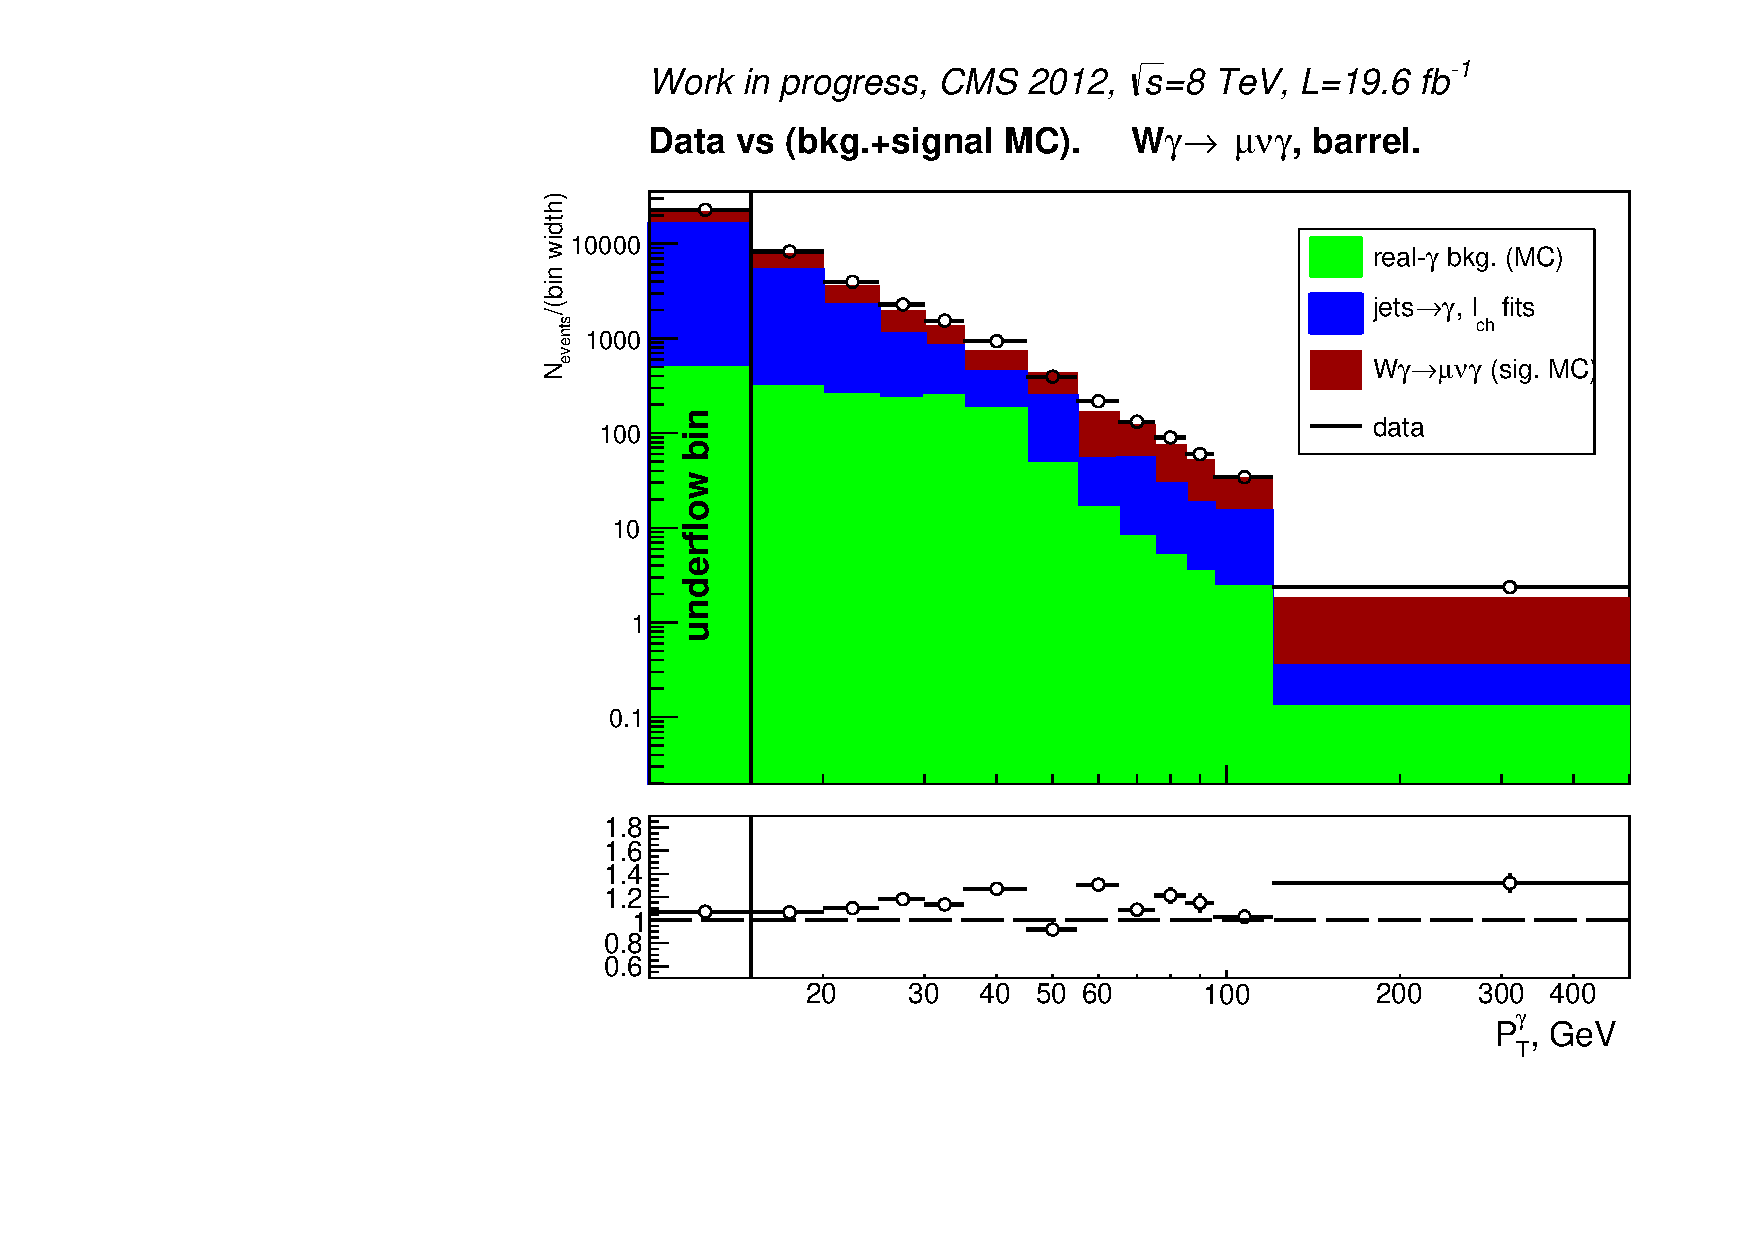
\includegraphics[width=0.30\textwidth]{../figs/figs_v11/MUON_WGamma/PrepareYields/c_DATAvsBkgPlusSigMCc_MUON_WGamma_TEMPL_CHISO_UNblind__Barrel__phoEt.pdf}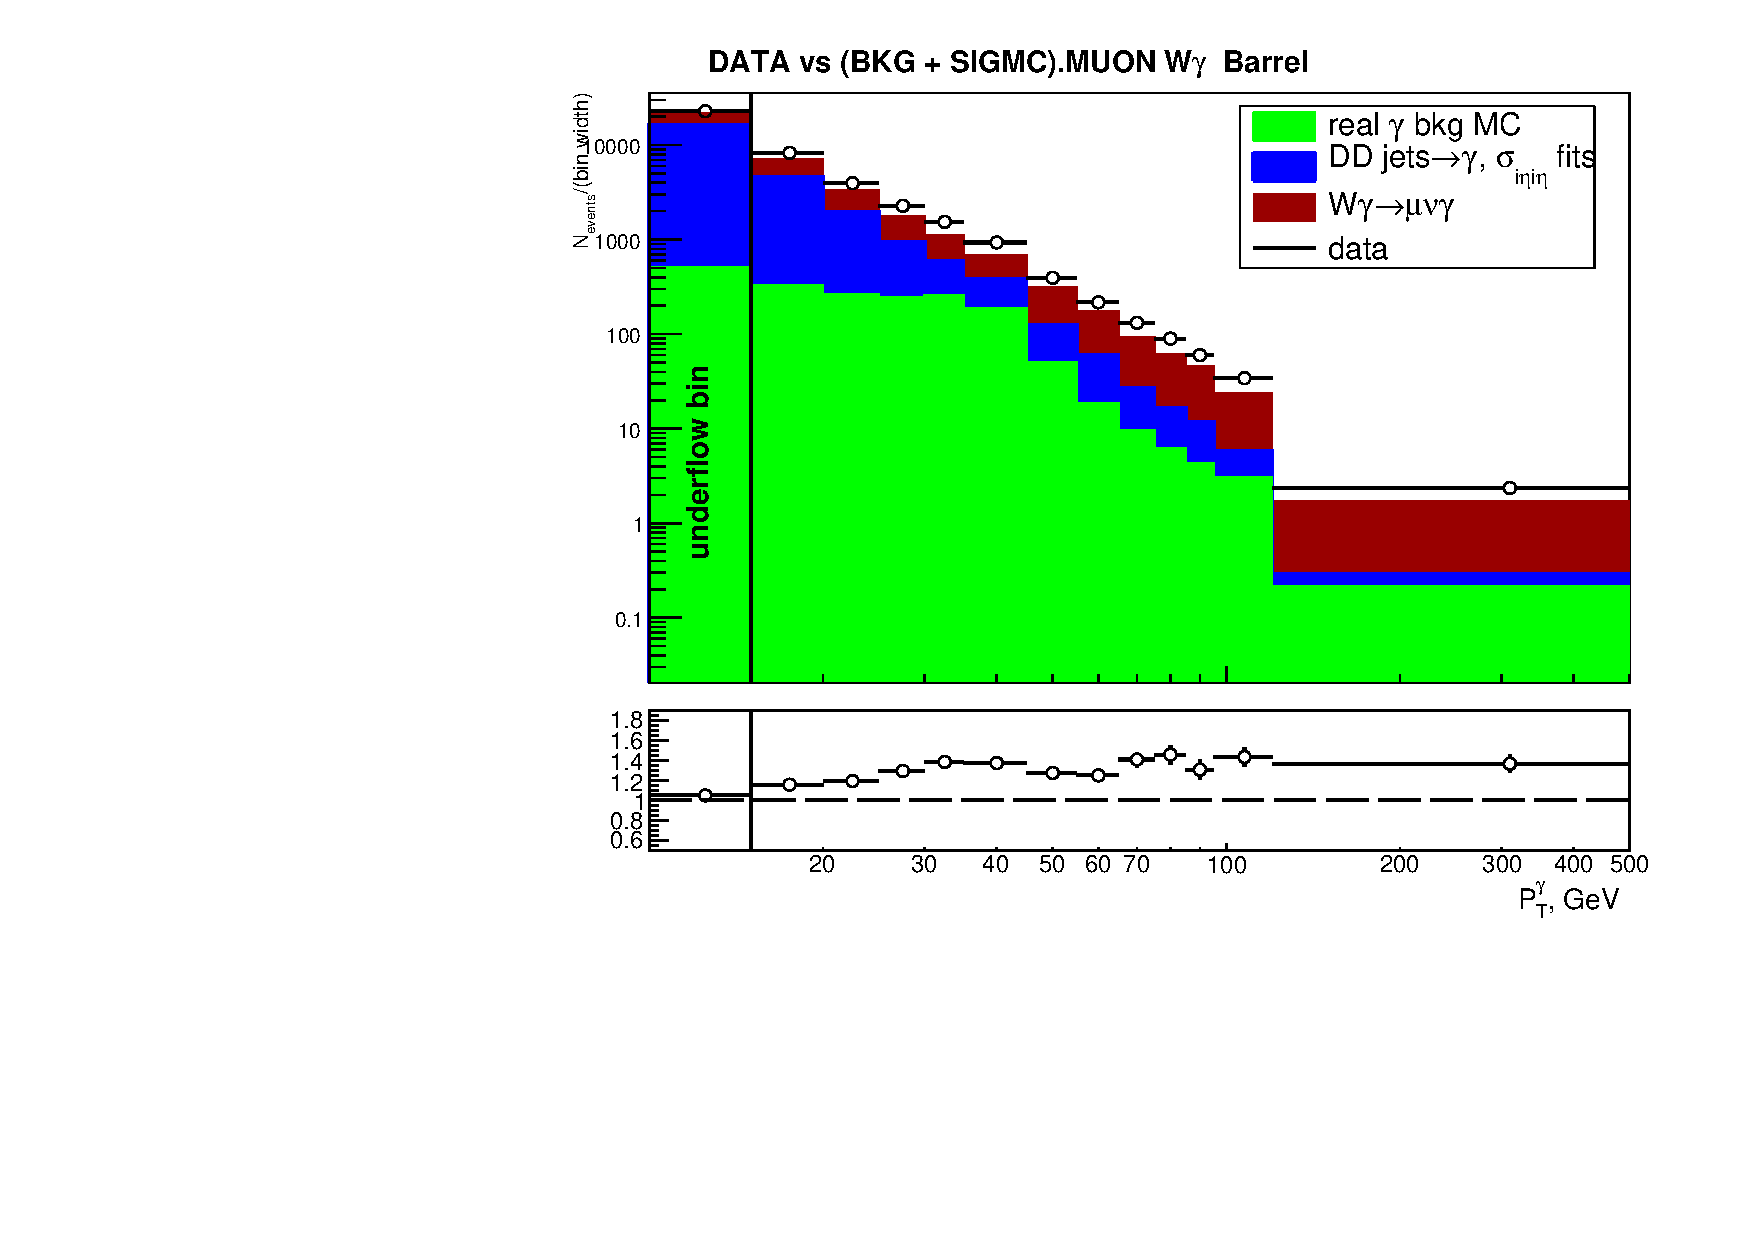
\includegraphics[width=0.30\textwidth]{../figs/figs_v11/MUON_WGamma/PrepareYields/c_DATAvsBkgPlusSigMCc_MUON_WGamma_TEMPL_SIHIH_UNblind__Barrel__phoEt.pdf}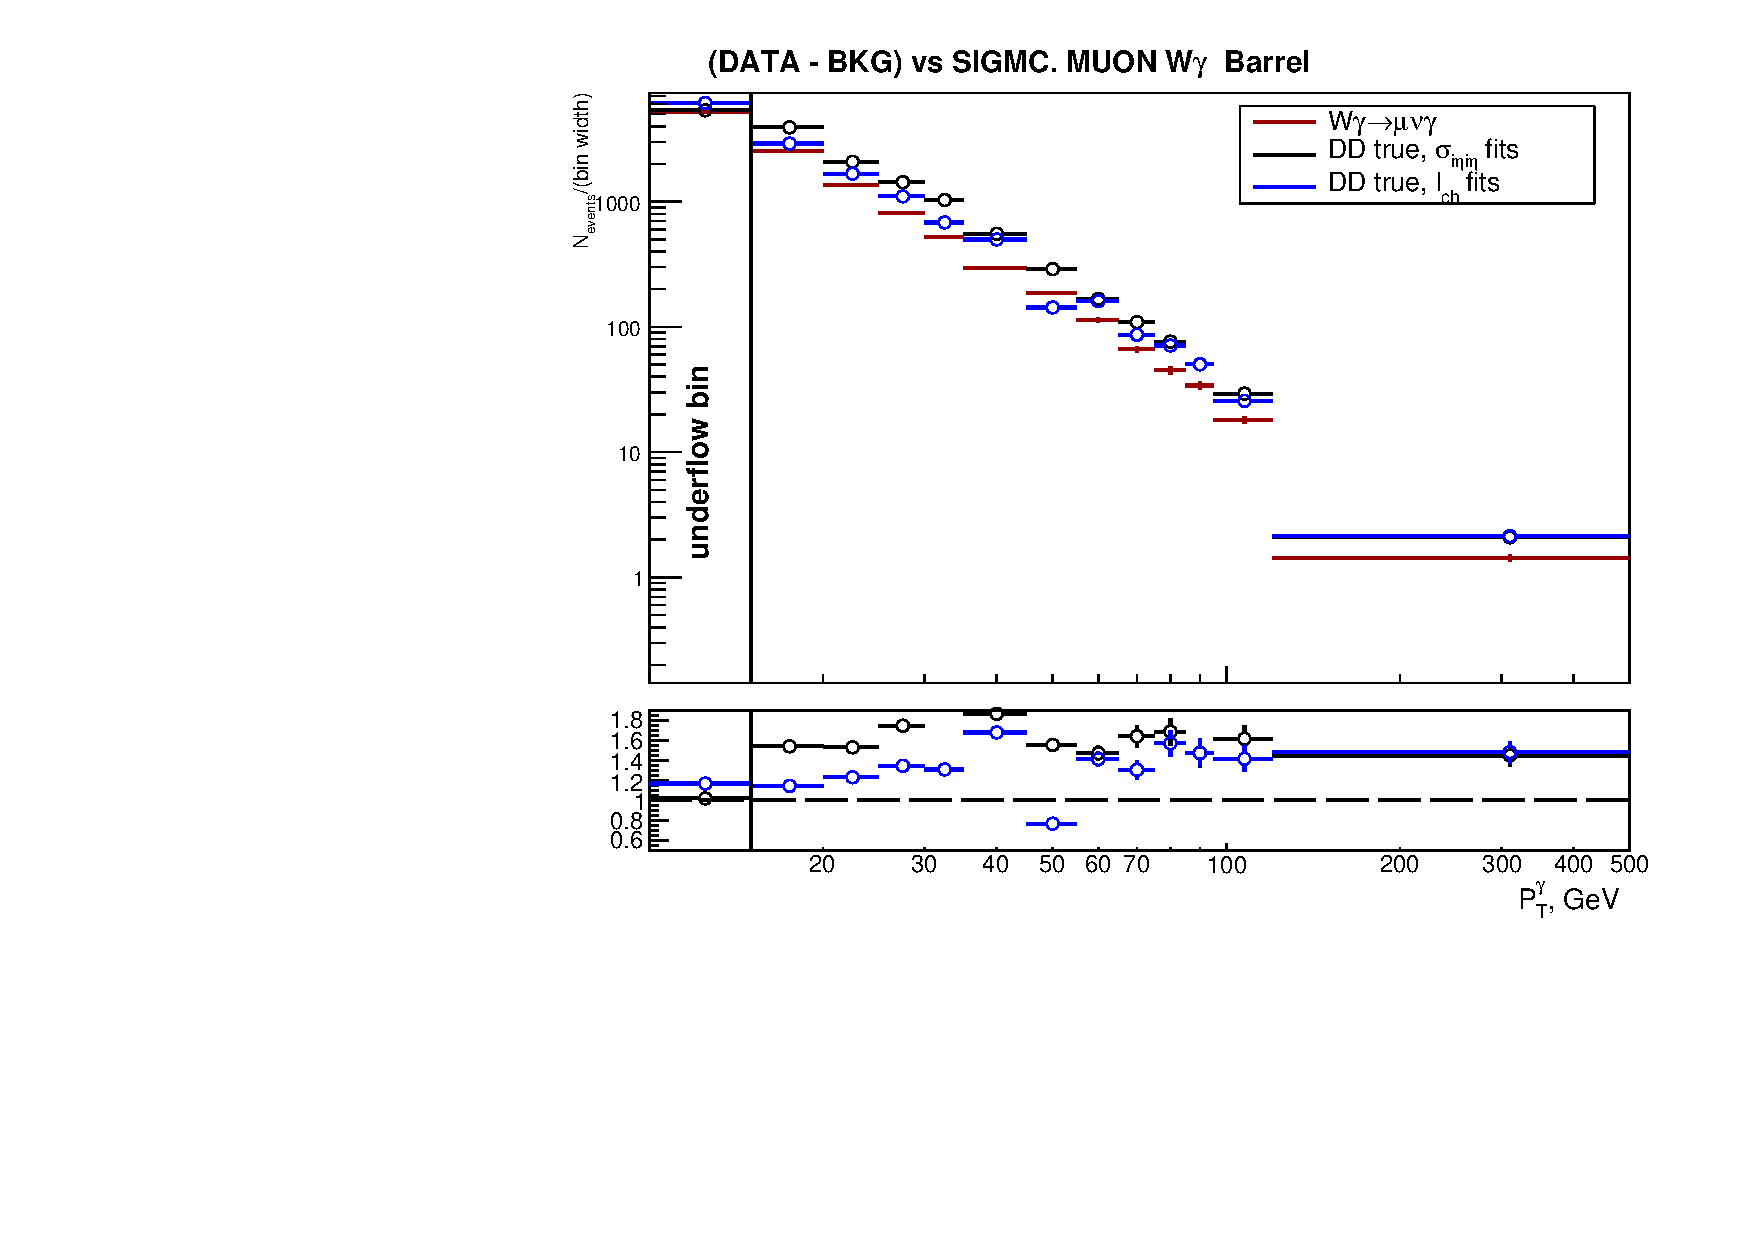
\includegraphics[width=0.30\textwidth]{../figs/figs_v11/MUON_WGamma/PrepareYields/c_BkgSubtrDATAvsSIGMC_c_MUON_WGamma__UNblind__Barrel__phoEt.pdf}\\
       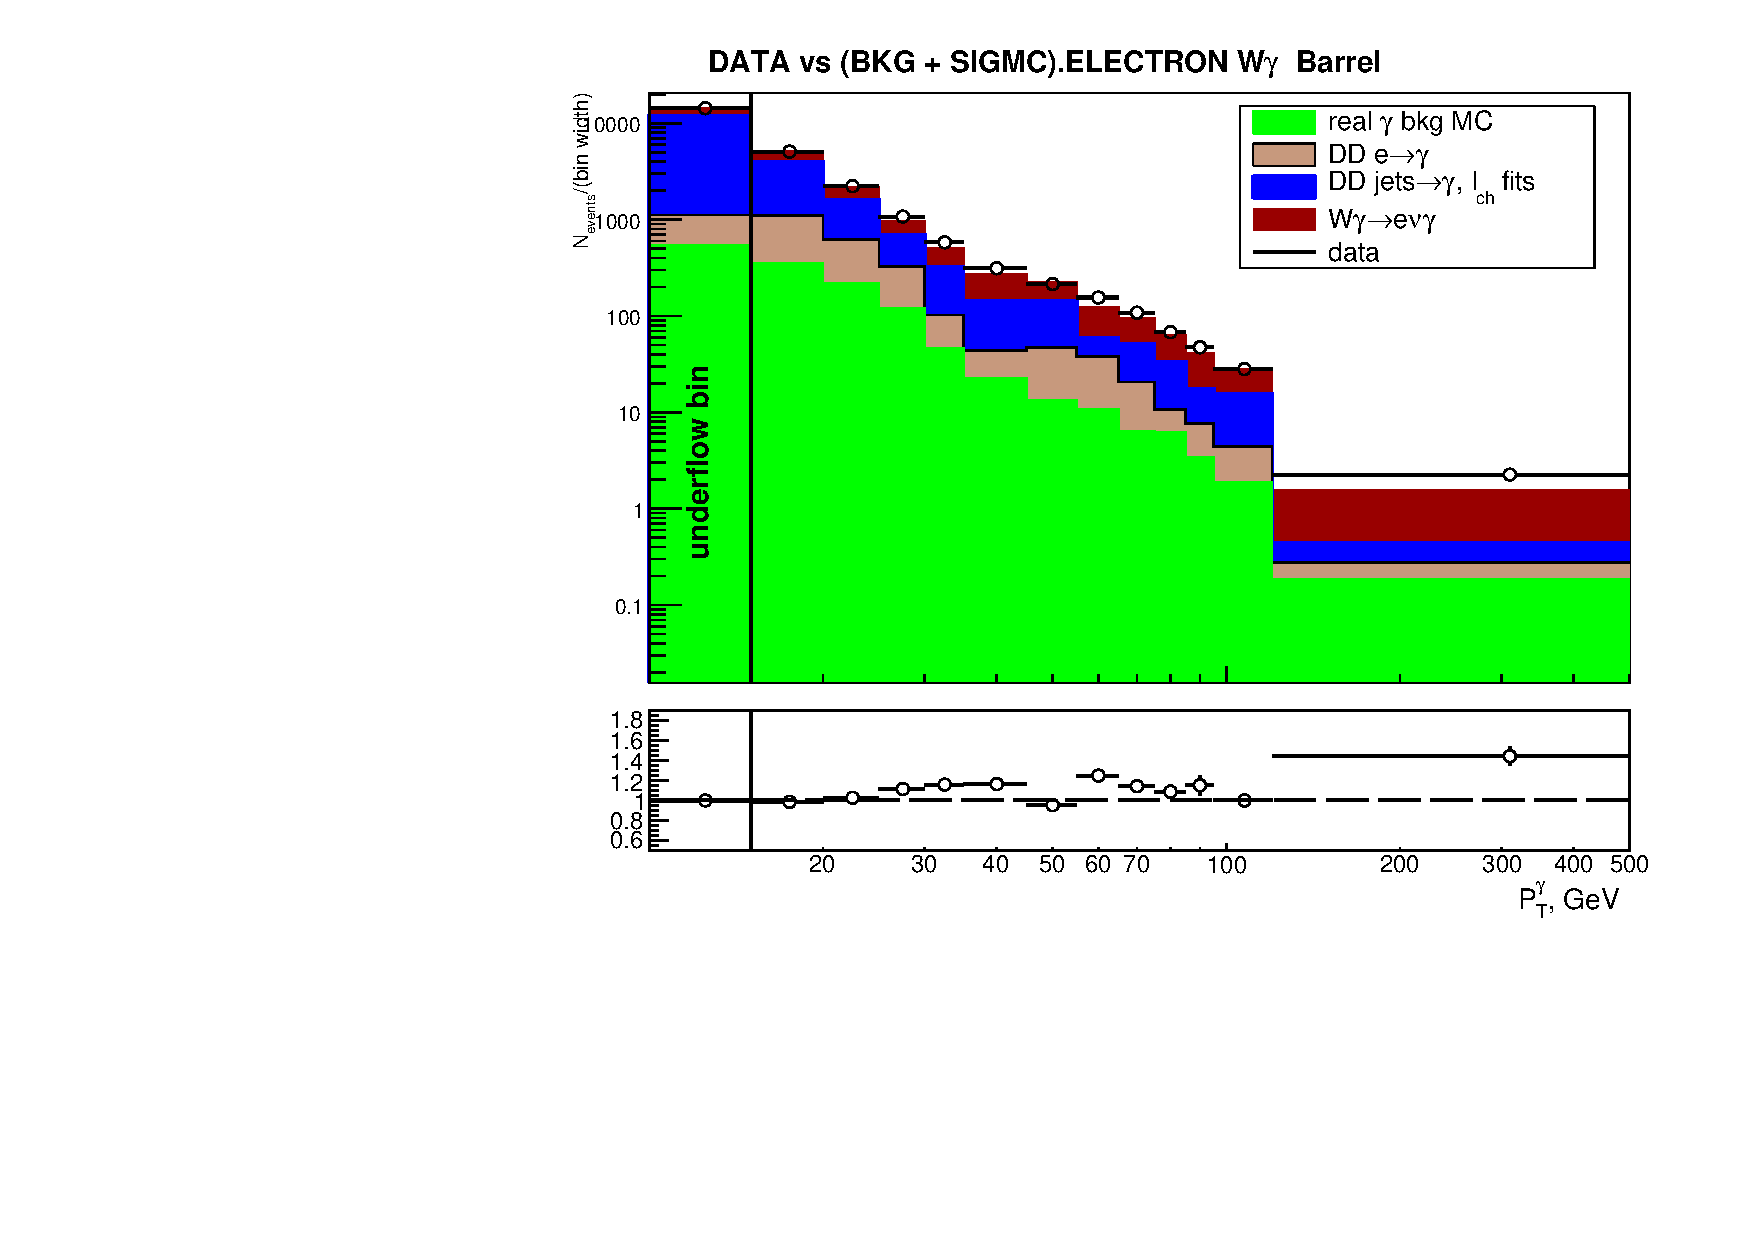
\includegraphics[width=0.30\textwidth]{../figs/figs_v11/ELECTRON_WGamma/PrepareYields/c_DATAvsBkgPlusSigMCc_ELECTRON_WGamma_TEMPL_CHISO_UNblind__Barrel__phoEt.pdf}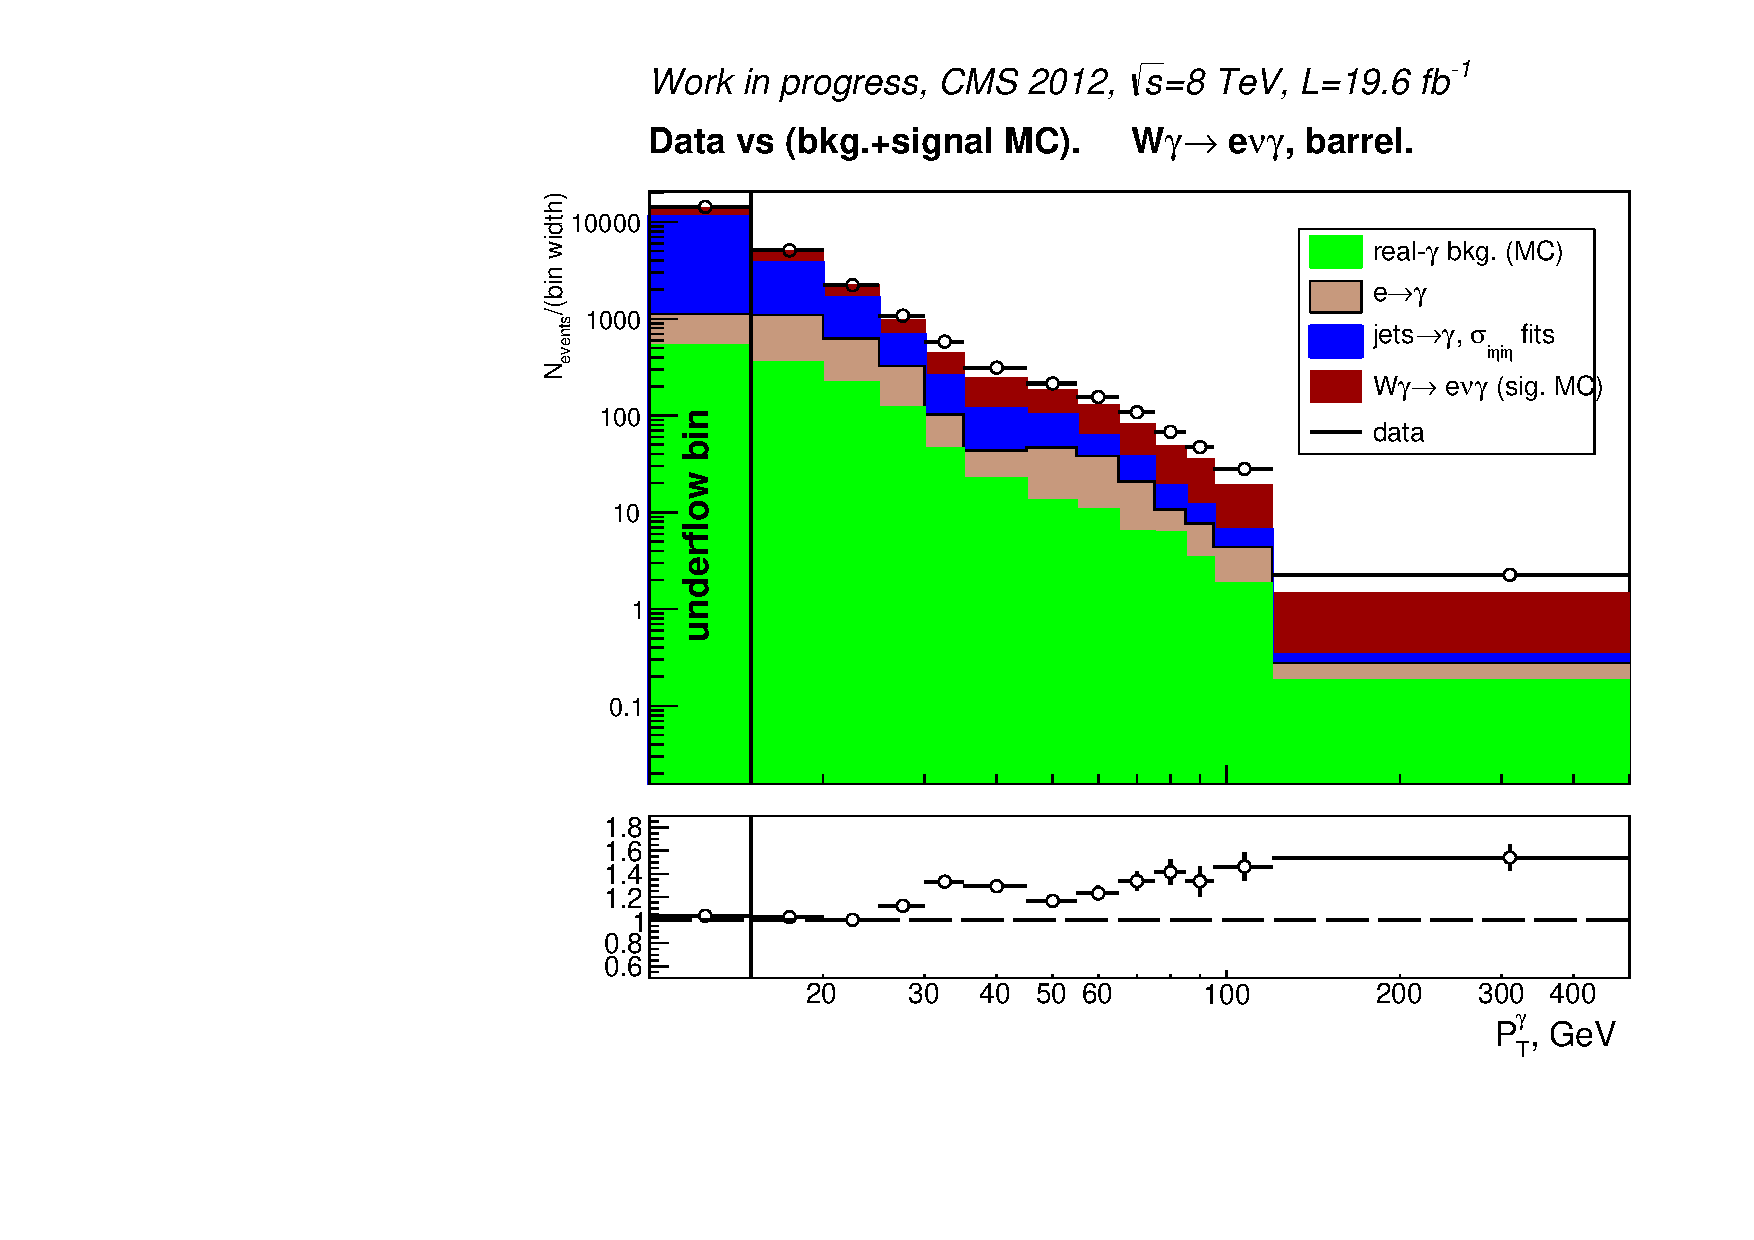
\includegraphics[width=0.30\textwidth]{../figs/figs_v11/ELECTRON_WGamma/PrepareYields/c_DATAvsBkgPlusSigMCc_ELECTRON_WGamma_TEMPL_SIHIH_UNblind__Barrel__phoEt.pdf}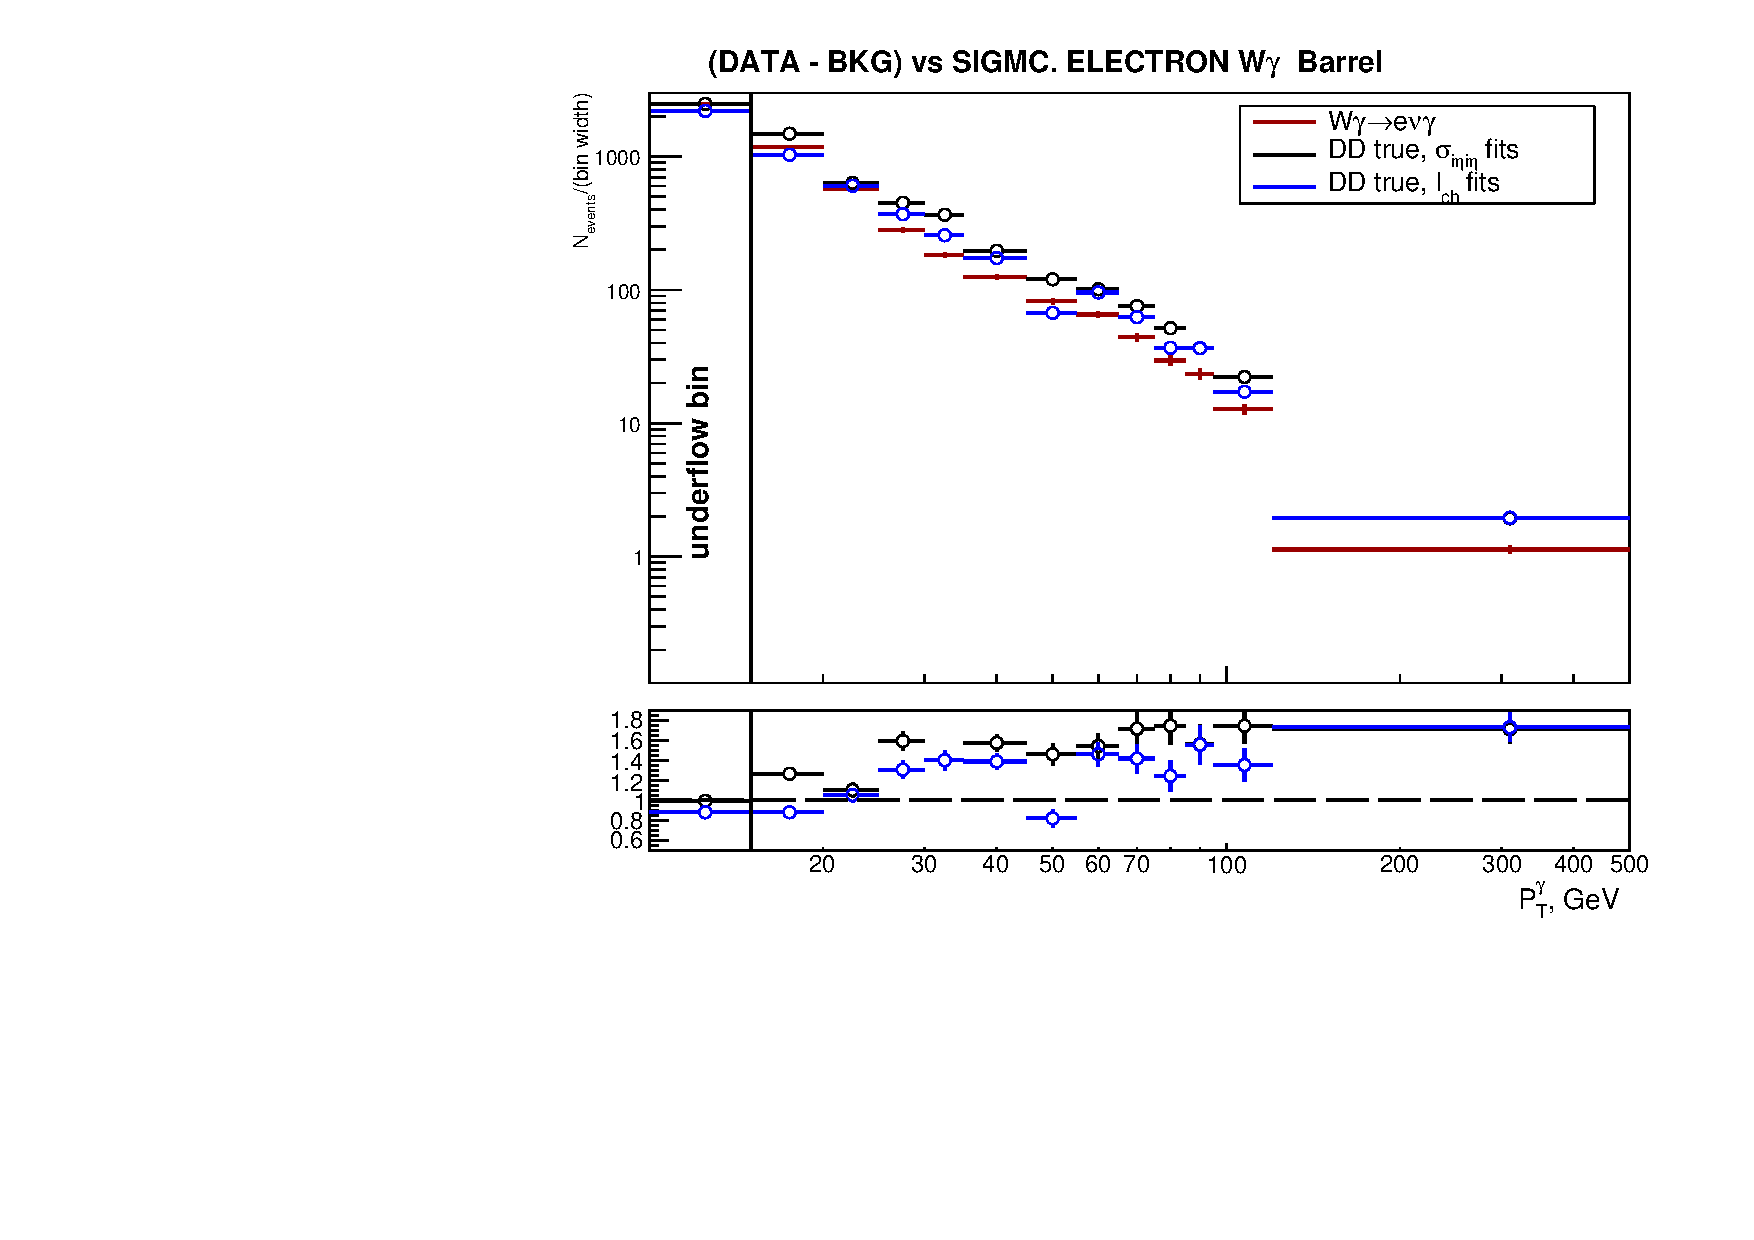
\includegraphics[width=0.30\textwidth]{../figs/figs_v11/ELECTRON_WGamma/PrepareYields/c_BkgSubtrDATAvsSIGMC_c_ELECTRON_WGamma__UNblind__Barrel__phoEt.pdf}\\
    \end{center}
  \end{figure}
\end{frame}%{$jets \rightarrow \gamma$ Background Subtraction. Plots, W$\gamma$}

\begin{frame}\frametitle{Other Corrections}

\begin{table}[h]
  \tiny
  \begin{center}
  \begin{tabular}{|l|c|c|}
    \hline
          & \multicolumn{2}{|c|}{Algebraic representation for} \\ 
     Step & \multicolumn{2}{|c|}{the measurement of} \\ 
          & $d\sigma/dP_{T}^{\gamma}$ & $\sigma$ \\ \hline
    select events & {\bfseries{$N_{sel}^j$}} &    {\bfseries{$N_{sel}$}}       \\ \hline
    subtract background & {\bfseries{$N_{sign}^j = N_{sel}^j - N_{bkg}^j$}} &    {\bfseries{$N_{sign}=N_{sel}-N_{bkg}$}}       \\ \hline
    \multicolumn{3}{|c|}{ } \\  
    \multicolumn{3}{|c|}{NEXT MEASUREMENT STEPS:} \\  
    \multicolumn{3}{|c|}{ } \\ \hline 
    {\bfseries\color{blue}{unfold}}   & {\color{blue}$N_{A\times\epsilon}^i = U_{ij} \cdot N_{sign}^j$} &    $-$       \\ \hline
    {\bfseries\color{blue}{correct for eff X acc}} & {\color{blue}$N_{true}^i = \frac{N_{A\times\epsilon}^i}{(A \times\epsilon)^i}$} &  {\color{blue}$N_{true}=\frac{N_{sign}}{A\times\epsilon}$}       \\ \hline
    compute cross section & $ \left( \frac{d\sigma}{dP_{T}^\gamma} \right) ^i = \frac{N_{true}^i}{L \cdot (\Delta P_T^\gamma)^i}$  &  $\sigma = N_{true}/L$       \\ \hline
    \multicolumn{3}{|l|}{estimate systematic uncertainties }         \\ \hline
  \end{tabular}
  \label{tab:analysisOutline}
  \end{center}
\end{table}

\scriptsize
{\bfseries{Detector resolution unfolding}} (step {\bfseries\color{blue}{``unfold''}}): 
  \begin{itemize} 
    \tiny
    \item {\bfseries{Effect:}} bin-to-bin migration during the $P_T^{\gamma}$ reconstruction; 
    \item {\bfseries{Method:}} D'Agostini, signal MC sample is used;
    \item {\bfseries{Note:}} uncertainties across difffent $P_T^{\gamma}$ bins become correlated.
  \end{itemize}

{\bfseries{Efficiency and Acceptance}} (step {\bfseries\color{blue}{``correct for eff X acc''}}): 
  \begin{itemize} 
    \tiny
    \item {\bfseries{Effect (main):}} lose signal events due to selection criteria applied;
    \item {\bfseries{Method:}} bin-by-bin correction by $A\times\epsilon$, constants prepared using signal MC sample;
    \item {\bfseries{Note:}} efficiencies between data and MC differ (next slide).
  \end{itemize}

\end{frame}%{Other Corrections}

\begin{frame}\frametitle{Efficiency Scale Factors}

\tiny
The scale factors (SF) $\rho = \frac{\epsilon_{data}}{\epsilon_{MC}}$. SF are applied as weights on each event in each MC sample.

\begin{table}[h]
  \tiny
  \begin{center}
   \begin{tabular}{|c|c|}
\hline
 type of candidate                  &   full event SF\\ 
 $W\gamma\rightarrow\mu\nu\gamma$   &   $\rho^{\mu}_{ID\_iso} \times \rho^{\gamma}_{ID}$    \\
 $W\gamma\rightarrow e\nu\gamma$    &   $\rho^{e}_{ID} \times \rho^{\gamma}_{ID}\times \rho^{\gamma}_{PSV}$       \\ \hline
  \end{tabular}
  \label{tab:SFs_Applied}
  \end{center}
\end{table}
Provided by POG: $\rho^{\mu}_{ID\_iso}$, $\rho^{\gamma}_{ID}$,  $\rho^{e}_{ID}$;       provided by $W\gamma\gamma$ measurement: $\rho^{\gamma}_{PSV}$

{\begin{center}$\rho^{\gamma}_{ID}$: \end{center}}
\begin{table}[h]
  \tiny
  \begin{center}
   \begin{tabular}{|c|c|c|c|c|}
\hline
 $P_T^{\gamma}$  & $|\eta^{\gamma}|\leq 0.80$ & $0.80<|\eta^{\gamma}|\leq 1.44$ & $1.57<|\eta^{\gamma}|\leq 2.00$ & $|\eta^{\gamma}|> 2.00$\\ \hline
15-20          & 0.95$\pm$0.02   & 0.99$\pm$0.02        & 1.00$\pm$0.02        & 1.02$\pm$0.02 \\ \hline
20-30          & 0.96$\pm$0.01   & 0.97$\pm$0.01        & 0.98$\pm$0.01        & 1.00$\pm$0.01 \\ \hline
30-40          & 0.98$\pm$0.01   & 0.98$\pm$0.01        & 0.99$\pm$0.01        & 1.00$\pm$0.01 \\ \hline
40-50          & 0.98$\pm$0.01   & 0.98$\pm$0.01        & 1.00$\pm$0.01        & 1.01$\pm$0.01 \\ \hline
$>$50          & 0.98$\pm$0.01   & 0.98$\pm$0.01        & 1.00$\pm$0.01        & 1.01$\pm$0.01 \\ \hline
  \end{tabular}
  \label{tab:SFs_PhotonID}
  \end{center}
\end{table}

{\begin{center}$\rho^{\gamma}_{PSV}$: \end{center}}
\begin{table}[h]
  \tiny
  \begin{center}
   \begin{tabular}{|c|c|c|}
\hline
 $P_T^{\gamma}$  & barrel              & endcap \\ \hline
15-20          & 0.996$\pm$0.020     & 0.960$\pm$0.041 \\ \hline
20-25          & 0.994$\pm$0.024     & 0.977$\pm$0.051 \\ \hline
25-30          & 0.996$\pm$0.030     & 0.951$\pm$0.062 \\ \hline
30-40          & 0.999$\pm$0.033     & 1.029$\pm$0.081 \\ \hline
40-50          & 1.009$\pm$0.073     & {\bfseries\color{blue}{0.971$\pm$0.150}} \\ \hline
50-70          & {\bfseries\color{blue}{0.993$\pm$0.128}}     & {\bfseries\color{blue}{0.965$\pm$0.294}} \\ \hline
$>$70          & {\bfseries\color{blue}{1.047$\pm$0.111}}     & {\bfseries\color{blue}{1.145$\pm$0.371}} \\ \hline

  \end{tabular}
  \label{tab:SFs_PhotonPixelSeedVeto}
  \end{center}
\end{table}


\end{frame}%{Efficiency Scale Factors}

\begin{frame}\frametitle{Uncertainties (Including ``unfolding'' step)}
\scriptsize{\bfseries{Statistical:}} \tiny{limited statistical power of the $W\gamma$-selected dataset}\\
\scriptsize{\bfseries{Systematic:}} \tiny{all other effects including limited stat. of control datasets and MC datasets}\\

  \begin{table}[h]
  \tiny
  \begin{center}
  \begin{tabular}{|l|c|c|}
    \hline
          & \multicolumn{2}{|c|}{Statistical uncertainty propagation} \\ 
     Step & \multicolumn{2}{|c|}{for the measurement of} \\
          & $d\sigma/dP_{T}^{\gamma}$ & $\sigma$ \\ \hline

    select events & $N_{sel}^j \pm \Delta N_{sel}^j$ &    $N_{sel} \pm \Delta N_{sel}$       \\ 
                  & {\color{blue}$\Delta N_{sel}^j = \sqrt{N_{sel}^j}$} &  {\color{blue}$\Delta N_{sel} = \sqrt{N_{sel}}$}   \\ \hline

    subtract background & $N_{sign}^j = N_{sel}^j - N_{bkg}^j$ &    $N_{sign}=N_{sel}-N_{bkg}$       \\ 
                        & {\color{blue}$\Delta N_{sign}^j = \Delta N_{sel}^j$} &    {\color{blue}$\Delta N_{sign} = \Delta N_{sel}$}   \\ \hline

    unfold   & $N_{A\times\epsilon}^i = U_{ij} \cdot N_{sign}^j$ &           \\ 
             & {\color{blue}$\Delta N_{A\times\epsilon}^i$: diagonal elements} &    $-$       \\ 
             & {\color{blue}of the error matrix} &           \\ \hline

    correct for eff X acc & $N_{true}^i = \frac{N_{A\times\epsilon}^i}{(A \times\epsilon)^i}$ &  $N_{true}=\frac{N_{sign}}{A\times\epsilon}$       \\ 
                          & {\color{blue}$\Delta N_{true}^i = \frac{\Delta N_{A\times\epsilon}^i}{(A \times\epsilon)^i}$} &  {\color{blue}$\Delta N_{true}=\frac{\Delta N_{sign}}{A\times\epsilon}$}       \\ \hline

    compute cross section & $ \left( \frac{d\sigma}{dP_{T}^\gamma} \right) ^i = \frac{N_{true}^i}{L \cdot (\Delta P_T^\gamma)^i}$  &  $\sigma = N_{true}/L$       \\ 
                          & {\color{blue}$ \Delta \left[ \left( \frac{d\sigma}{dP_{T}^\gamma} \right) ^i \right]= \frac{\Delta N_{true}^i}{L \cdot (\Delta P_T^\gamma)^i}$ } &  {\color{blue}$\Delta\sigma = \DeltaN_{true}/L$   }    \\ \hline

  \end{tabular}
  \end{center}
\end{table}

\end{frame}%Systematic Uncertainties. Introduction

\begin{frame}\frametitle{Relative Uncertainties [\%]\\
  on the $W\gamma\rightarrow e\nu\gamma$ Cross Section}
\footnotesize
Diagonal elements of error matrices only
\begin{table}[h]
  \tiny
  \begin{center}
  %\caption{Relative uncertainties [\%].}
   \begin{tabular}{|c|c|c|c|c|c|c|c|c|c|}
   \hline
                  &       & \multicolumn{8}{|c|}{systematic uncertainties}     \\
    $P_T^{\gamma}$, & stat. & \multicolumn{3}{|c|}{\color{blue}\bfseries{related to jets$\rightarrow\gamma$}} &  &  &  &  & \\
    GeV           & unc.  & {\color{blue}\bfseries{$N_{Ich}$ vs}}          &{\color{blue}\bfseries{$Z\gamma$ MC}} & templ. & {\color{blue}\bfseries{SFs}} & lumi &$e\rightarrow\gamma$ & other & total\\ 
                  &       & {\color{blue}\bfseries{$N_{\sigma{i\eta i\eta}}$}} & {\color{blue}\bfseries{norm.}}       & stat.  &  &  & &  & syst.\\ \hline
    $>$15  & 2 & 15 & {\color{blue}\bfseries{35}} & 5 & 19 & 3 & 4 & 5 & 44 \\ \hline
%    10-15 & 4 & 73 & 20 & 16 & 1 & 3 & 2 & 8 & 78 \\ \hline
    15-20 & 8 & {\color{blue}\bfseries{80}} & 27 & 19 & 17 & 3 & 18 & 11 & 90 \\ \hline
    20-25 & 7 & {\color{blue}\bfseries{38}} & 20 & 14 & 12 & 3 & 11 & 10 & 48 \\ \hline
    25-30 & 5 & {\color{blue}\bfseries{25}} & 16 & 12 & 14 & 3 & 8 & 8 & 36 \\ \hline
    30-35 & 5 & {\color{blue}\bfseries{35}} & 14 & 12 & 14 & 3 & 3 & 8 & 42 \\ \hline
    35-45 & 3 & 14 & 13 & 8 & {\color{blue}\bfseries{18}} & 3 & 2 & 7 & 28 \\ \hline
    45-55 & 8 & {\color{blue}\bfseries{53}} & 20 & 22 & 36 & 3 & 7 & 11 & 71 \\ \hline
    55-65 & 7 & 17 & 12 & 30 & {\color{blue}\bfseries{44}} & 3 & 5 & 10 & 58 \\ \hline
    65-75 & 7 & 23 & 15 & 32 & {\color{blue}\bfseries{44}} & 3 & 4 & 11 & 61 \\ \hline
    75-85 & 8 & 32 & 17 & 27 & {\color{blue}\bfseries{44}} & 3 & 6 & 13 & 64 \\ \hline
    85-95 & 9 & 9 & 7 & 9 & {\color{blue}\bfseries{40}} & 3 & 8 & 14 & 44 \\ \hline
    95-120 & 7 & 19 & 9 & 14 & {\color{blue}\bfseries{44}} & 3 & 5 & 11 & 51 \\ \hline
    120-500 & 4 & 12 & 6 & 24 & {\color{blue}\bfseries{39}} & 3 & 1 & 9 & 48 \\ \hline
  \end{tabular}
  \label{tab:systInPercent_ELECTRON_WGamma}
  \end{center}
\end{table}
\end{frame}%Systematic Uncertainties. Table. Electron channel

\begin{frame}\frametitle{Major Sources of the Systematic Uncertainties}

\footnotesize{\bfseries{Related to jets$\rightarrow\gamma$ background estimation:}}
  \begin{itemize}
     \scriptsize
     \item {\bfseries{Bias in Template Shape and Fit Machinery:}} 
        \begin{itemize}
          \tiny
          \item Estimate as $|N_{Ich}-N_{\sigma{i\eta i\eta}}|$.
         \end{itemize}
     \item {\bfseries{$Z\gamma$ MC Normalization:}}
        \begin{itemize}
          \tiny
          \item Assign uncertainty on the $Z\gamma$ normalization of $\Delta N=$4.6\% (CMS published $Z\gamma$ measurement);
          \item Prepare fake-$\gamma$ templates with $Z\gamma$ MC normalizations of $N\pm\Delta N$;
          \item Perform fits with such deviated templates;
          \item Assign the spread among the three results as an uncertainty.
        \end{itemize}
     \item {\bfseries{Statistical Power of Templates:}}
       \begin{itemize}
          \tiny
          \item Randomize fake-$\gamma$ templates 100 times with Gaussian distribution;
          \item Perform fits with such deviated templates;
          \item Take the Standard deviation of 100 fit results as an uncertainty;
          \item Same for real-$\gamma$ templates (except randomize 20 times, not 100).
       \end{itemize}
     \item Propagate each of three uncertainties through unfolding and other corrections.
  \end{itemize}

\footnotesize{- - - - - - - - - - - - - - - - - - - -}\\
\footnotesize{\bfseries{Related to PixelSeedVeto SF (electron channel only):}}
  \begin{itemize}
  \begin{itemize}
     \tiny
     \item Change SF by $\pm \Delta[SF]$;
     \item From signal MC, obtain new constants for $A \times \epsilon$ and unfolding corrections;
     \item Compute two new cross section values corresponding to $\pm \Delta[SF]$;
     \item Assign the spread among three cross section values as an uncertainty. 
  \end{itemize}
  \end{itemize}
\end{frame}%Major Sources of the Systematic Uncertainties

\begin{frame}\frametitle {Cross Checks for Jets$\rightarrow\gamma$ Background Estimation}
\tiny

\begin{table}[h]
  \tiny
  \begin{center}
    \begin{tabular}{|l|c|c|c|}
      \hline
      Checks$\rightarrow$  & {\bfseries{- - - Simple MC closure - - -}} &  {\bfseries{- - - - - MC realistic - - - - -}}   & {\bfseries{- - - - - - - $Z\gamma$ data - - - - - - -}} \\ \hline

      Templates & \multicolumn{2}{|c|}{MC samples}                 &  $Z\gamma$ FSR and ISR data \\ 
                & $W\gamma$ and $W$+jets &  $Z\gamma$ and DY+jets  &  (same as for $W\gamma$ meas.) \\ \hline

      Data-to-fit & \multicolumn{2}{|c|}{Mix MC samples}   &  $Z\gamma$-selected  \\ 
                  & $W\gamma$ and $W$+jets  & All $W\gamma$-selected  &  data \\ \hline

      Check & \multicolumn{3}{|c|}{Compare fit results of two methods to each other and to MC predictions} \\
                                                       &  &   &  Compute cross section  \\ 
                                                      &  &   &  and compare to CMS published \\ \hline
      Agreement & mostly good & slightly better than in data &  excellent \\ \hline
    \end{tabular}
  \end{center}
\end{table} 

\footnotesize{\bfseries{Reasons of discrepancies in the $W\gamma$ measurement:  }}
\scriptsize
\begin{itemize}
  \item Not accurate shape of templates; 
  \item Effect of a bias on the fit machinery.
\end{itemize}

\end{frame}%{cross checks}

\begin{frame}\frametitle{Limits on aTGC constants}
  \begin{figure}[htb]
    \begin{center}
       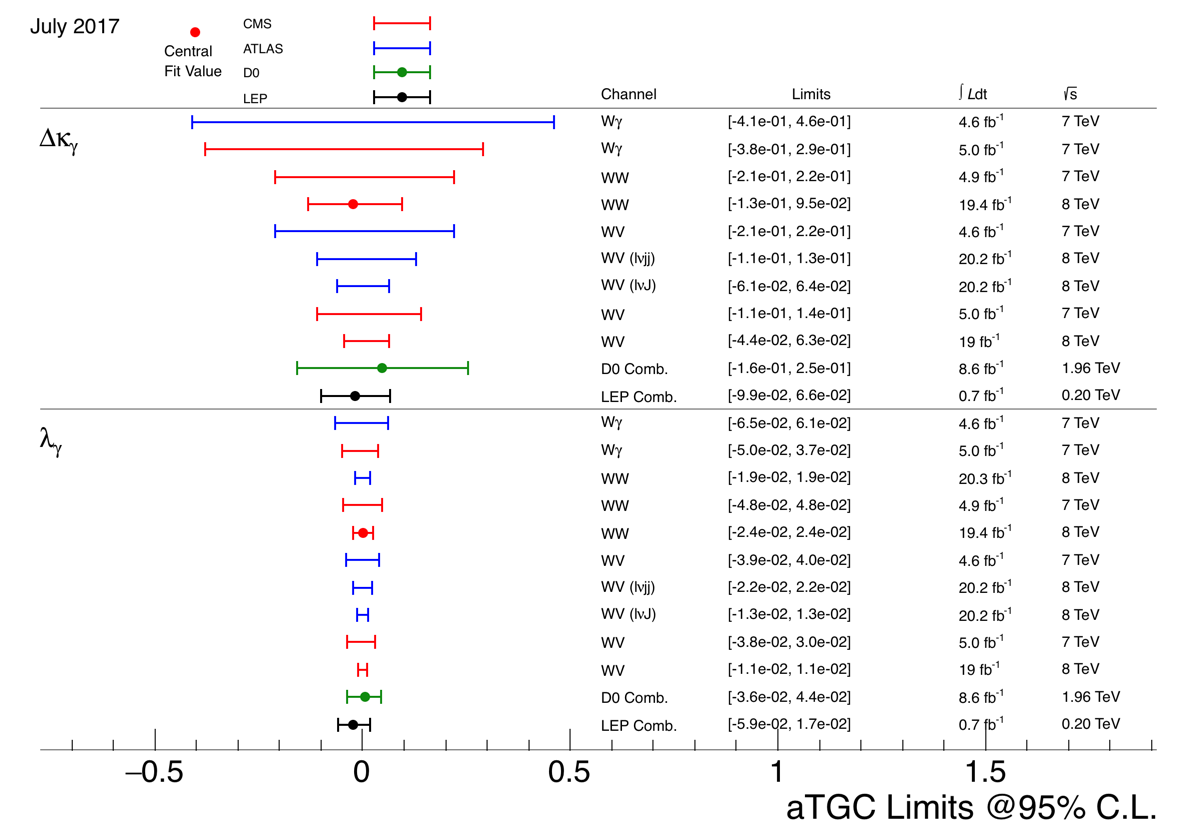
\includegraphics[width=0.70\textwidth]{../figs/ForPresentation/aTGC_cg.png} 
    \end{center}
  \end{figure}
  \scriptsize
  $WW$: $pp \rightarrow W^+ W^- \rightarrow l^+ \nu l^- \bar{\nu}$\\
  $WV$: ($pp \rightarrow WW \rightarrow l \nu$+jets) + ($pp \rightarrow WZ \rightarrow l \nu$+jets)
  \tiny
  https://twiki.cern.ch/twiki/bin/view/CMSPublic/PhysicsResultsSMPaTGC
\end{frame}%{WGamma, LO and NLO Feynman diagrams}


%\include{presentation_20160412_thesisEndorsement_BackupSlides}

\end{document}
